%% The following is a directive for TeXShop to indicate the main file
%%!TEX root = diss.tex

\chapter{An Interpretation of 3D Reconstruction}
\label{ch:3DRecon_Interp}
So far we have proposed a well-defined problem space for the 3D reconstruction problem, as well as a precise mapping from the problem space to the algorithm space. This section, we propose a proof-of-concept interpreter that translates the description to an appropriate algorithm that can give a reliable reconstruction result. In other words, the interpretation from a problem-centric description to a reliable reconstruction result must be shown. Both synthetic and real-world datasets are provided to evaluate the performance of the interpreter.

However, such an evaluation faces several challenges. First, the mapping does not pose very strict constraints on object's geometry, and an exhaustive evaluation would require a vast number of objects to reach a solid conclusion, which is not a practical approach. Second, we need a selection of algorithms that cover a wide range of problem space so that we can determine more convincingly if an unsuccessful result is due to lack of coverage or the limits of the interface.

To address the first challenge, we assume \textit{local interaction model}, which is not an uncommon assumption in vision community. Thus, geometric properties, such as concavity, that violate this assumption will not be considered. Thus, objects with shallow concavities are used for evaluation. For the second challenge, we need a selection of algorithms that cover a wide range of problem space. Aside from a Patch-based Multi-view Stereo algorithm, we implemented a Photometric Stereo and Structured Light technique as discussed in Chapter~\ref{ch:3DRecon_Mapping}. From the mapping developed in Chapter~\ref{ch:3DRecon_Mapping}, the selected algorithms cover a reasonably wide range of problem space, thus is sufficient to demonstrate the interface's ability to translate the descriptive model into a reconstruction. Further, it is relatively straightforward to incorporate new algorithms, as long as they are evaluated with the same problem conditions presented in Chapter~\ref{ch:3DRecon_Mapping}. This allows researchers to contribute novel algorithms to the interface once they become available.

% In Chapter~\ref{ch:3DRecon_Mapping}, we have established a mapping from a well defined problem space to a suite of algorithms by evaluating the performance of the selected algorithms under synthetic conditions. However, the claim that this mapping would help the users obtain a satisfactory reconstruction result given the correct problem conditions is still unclear. Thus a thorough evaluation is needed to validate the proposed interface.

This chapter is organized as follows: Section~\ref{sec:interp_eval_methodology} provides a roadmap of our evaluation that is centered around one key evaluation question. Section~\ref{sec:interp} proposes a proof-of-concept interpreter. Section~\ref{sec:eval_interp} addresses the evaluation question by demonstrating the robustness of the interpreter using synthetic and real-world datasets, where a satisfactory reconstruction result is returned given the correct description of the object.

% In order to validate the 3D reconstruction mapping derived from Chapter~\ref{ch:3DRecon_Mapping}, evaluation of the object centric model into appropriate solutions must be shown. Our interpreter is based on the direct evaluation of the performance of each 3D reconstruction algorithm under different conditions presented in Chapter~\ref{ch:3DRecon_Mapping}. From this analysis of how algorithms perform on objects which have different visual and geometric properties, an algorithm(s) can be definitively chosen based on which performed best on the training images.

\section{Evaluation Methodology}
\label{sec:interp_eval_methodology}
% This section formulates the methodology of evaluation. We start with the objective, which gives a brief introduction of what needs to be evaluated. Next, two key evaluation questions are proposed, with evaluation steps, criteria and expected outcomes to determine if the evaluation is successful.

% \subsection{Objective}
% [Develop a description (or access an existing version) of what is to be evaluated and how it is understood to work.]
This evaluation intends to demonstrate the robustness of the proof-of-concept interpreter using synthetic and real-world datasets.

% For our first goal, objects with varied degrees of shape (concavity) changes are used, and the corresponding results are compared to the mapping. We attempt to demonstrate if the mapping, to some extent, is robust to the changes of shape, and when it would fail to hold. For the second goal, we use synthetic and real-world objects to demonstrate that the interpreter can return a satisfactory result when provided with a correct description.

% \subsection{Frame}
% Set the parameters of the evaluation its purposes, key evaluation questions and the criteria and standards to be used.

% \subsubsection{Purpose}
% [What are the primary purposes and intended uses of the evaluation?]
% The evaluation intends to find out that the derived mapping can indeed find the algorithm that produces the best possible result from a suite of algorithms.

% \subsection{Key Evaluation Questions and Steps}
% [What are the high level questions the evaluation will seek to answer? How can these be developed?]

% The evaluation attempts to \textit{prove that the mapping can be extended to other objects with different geometries}, and \textit{demonstrate that the interface can return a satisfactory reconstruction result given a correct description}.

% \noindent\textbf{Data generation} the synthetic data is generated in Blender using the same setups presented in Chapter~\ref{ch:3DRecon_Mapping}. We consider the four property settings that represent four major classes of real-world objects from Chapter~\ref{ch:3DRecon_Taxo}.

% If that is not the case, we need to find out how robust each algorithm in within the mapping is with respect to concavity changes, and how concavity change affects the reconstruction results.

\subsubsection{Can the proof-of-concept interpreter return a satisfactory reconstruction given the correct description?}
Given a correct description of the object, the algorithm chosen by the proof-of-concept interpreter should give a successful reconstruction result. In this case, visual inspection is utilized to determine the quality of reconstruction result. More specifically, the result returned by the interface is compared to that of the baseline algorithm to determine if the quality is acceptable. As previously mentioned, the baseline method is chosen so that it always can provide a decent reconstruction under most circumstances.

% \noindent\textbf{Validation}: we need to demonstrate that the interpreter would return a reliable reconstructed model given the correct description, and a less successful model given an invalid description. The quality of the reconstruction is determined by comparing the result to the baseline method.

% \subsubsection{Criteria}
% Determine what `success' look like? What should be the criteria and standards for judging performance? Whose criteria and standards matter? What process should be used to develop agreement about these?

% \subsubsection{Steps}
% [Collect and retrieve data to answer descriptive questions about the activities of the project/programme/policy, the various results it has had, and the context in which it has been implemented.]

\section{Interpreter}
\label{sec:interp}
Our interface consists of three separate layers. The upper layer is the description of the problem condition. The middle layer is the interpreter which receives a description from the user and return an acceptable result. The bottom layer is the actual implementation of the algorithms. The interpreter is responsible for choosing an appropriate 3D reconstruction algorithm based on the description of the problem domain and additional requirements. Thus, it requires an understanding of algorithmic performance across difference ranges of problem space to create a suitable interpreter. There are many ways to use the mapping to interpret the problem description. We proposed a proof of concept interpreter that consists of two components: mapping and constraints.
\begin{figure}[!htbp]
\centering
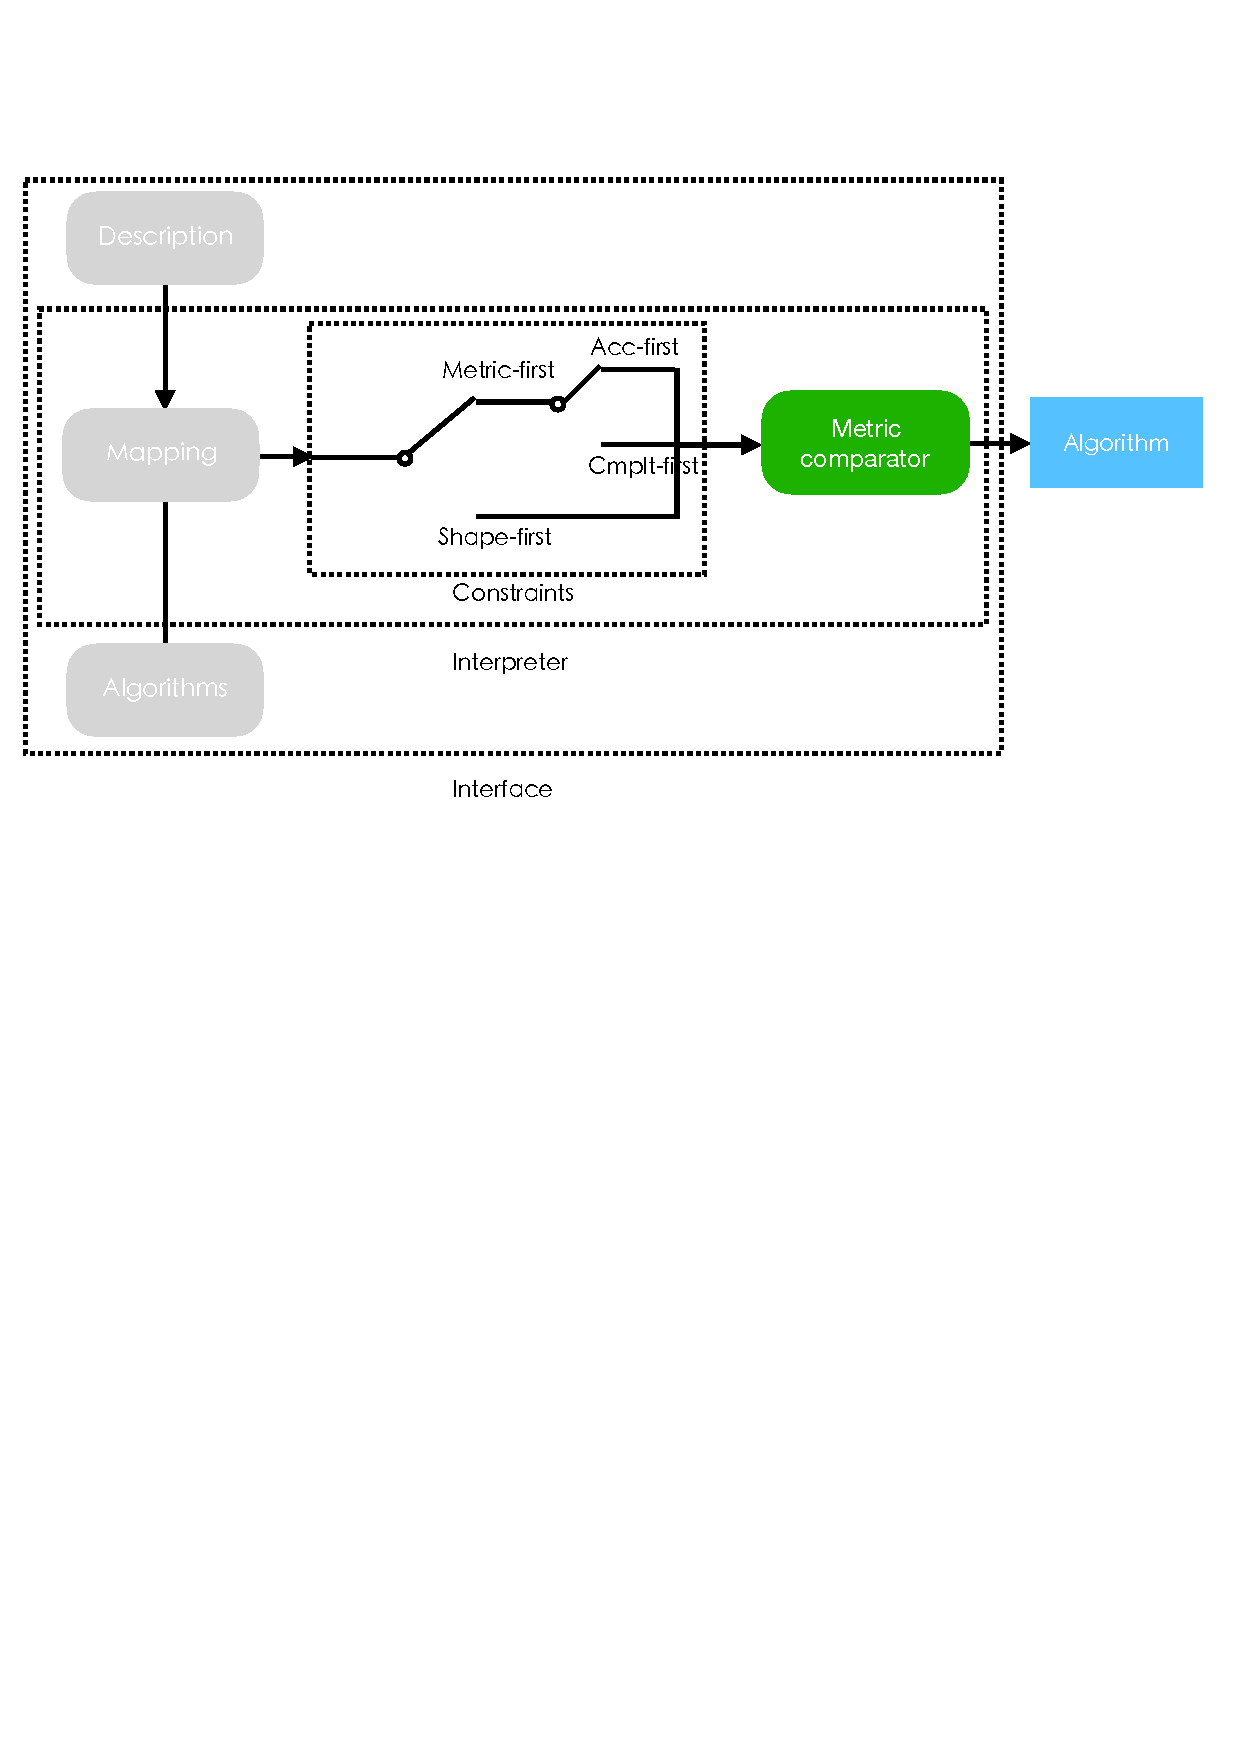
\includegraphics[width=0.8\textwidth]{interp/interpreter.pdf}
\caption{Two components of the Interpreter layer.}
\label{fig:interpreter_layer}
\end{figure}

The mapping constructed using the synthetic datasets from Chapter~\ref{ch:3DRecon_Mapping} provides us with a detailed understanding of the performance of algorithms under varied problem conditions. This allows us to select an appropriate algorithm based on a description of properties.
% When multiple algorithms are appropriate, we use a very simple ranking system based on the metrics: if one algorithm has the same completeness but is more accurate, or more complete and equally accurate, it is chosen over the others. (This ranking also allows us to define an efficiency versus accuracy tradeoff for the developer to use.) We could also choose to execute more than one algorithm and accept the results of the one which performed best - however measuring this may be challenging.

Next we turn to defining the constraints of the interface. Constraints are provided to allow the user to describe the expected result so that a model best resembling the user's request can be returned by the interface when multiple algorithms achieve satisfactory results. The following constraints are provided: 
\begin{itemize}
\item Depth-first/shape-first: methods that reconstructs surface orientations from a single viewpoint cannot retrieve the depth information, and thus are refered to as 2.5D reconstruction. Examples of this are Shape from Shading, Photometric Stereo, and Shape from (de)focus, \etc. However, these methods generally can reconstruct fine scale details, thus can achieve results with much higher quality. Intuitively, depth-first can return model with true depth information whereas shape-first prioritizes fine details over depth information.
\item Accuracy-first/completeness-first: methods that achieve high accuracy do not necessary achieve high completeness. In light of this, the user can choose an algorithm based on the priority level of accuracy and completeness.
\end{itemize}

Under our current interpreter, if a developer-defined description and constraints have more than one corresponding algorithm available, by default, depth-first has higher priority over quality-first, and accuracy has higher priority over completeness. Since GSL typically generates more accurate resutlts, the order of the algorithms is: GSL $>$ PMVS $>$ EPS.

\section{Overview of Datasets}
In this section, we introduce a synthetic and real-world dataset to evaluate the performance of the interpreter under varied problem conditions. To the best of our knowledge, there is few publicly available dataset that captures images for algorithms across different categories.

The synthetic dataset contains four objects, and the real-world dataset contains nine objects, as shown in Figure~\ref{}. It covers materials that represents the four problem conditions proposed in Chapter~\ref{ch:3DRecon_ProbSpace}: textureless, diffuse, bright (statue), textureless, mixed, bright (cup), textured, diffuse, bright (pot), textured, mixed, bright (vase). In terms of surface shapes, we have focused mainly on objects with simple geometric properties, namely, smoothly curved surfaces, surfaces with shallow concavities.

\begin{figure*}[!htbp]
\centering
\begin{tabular}{ccc}
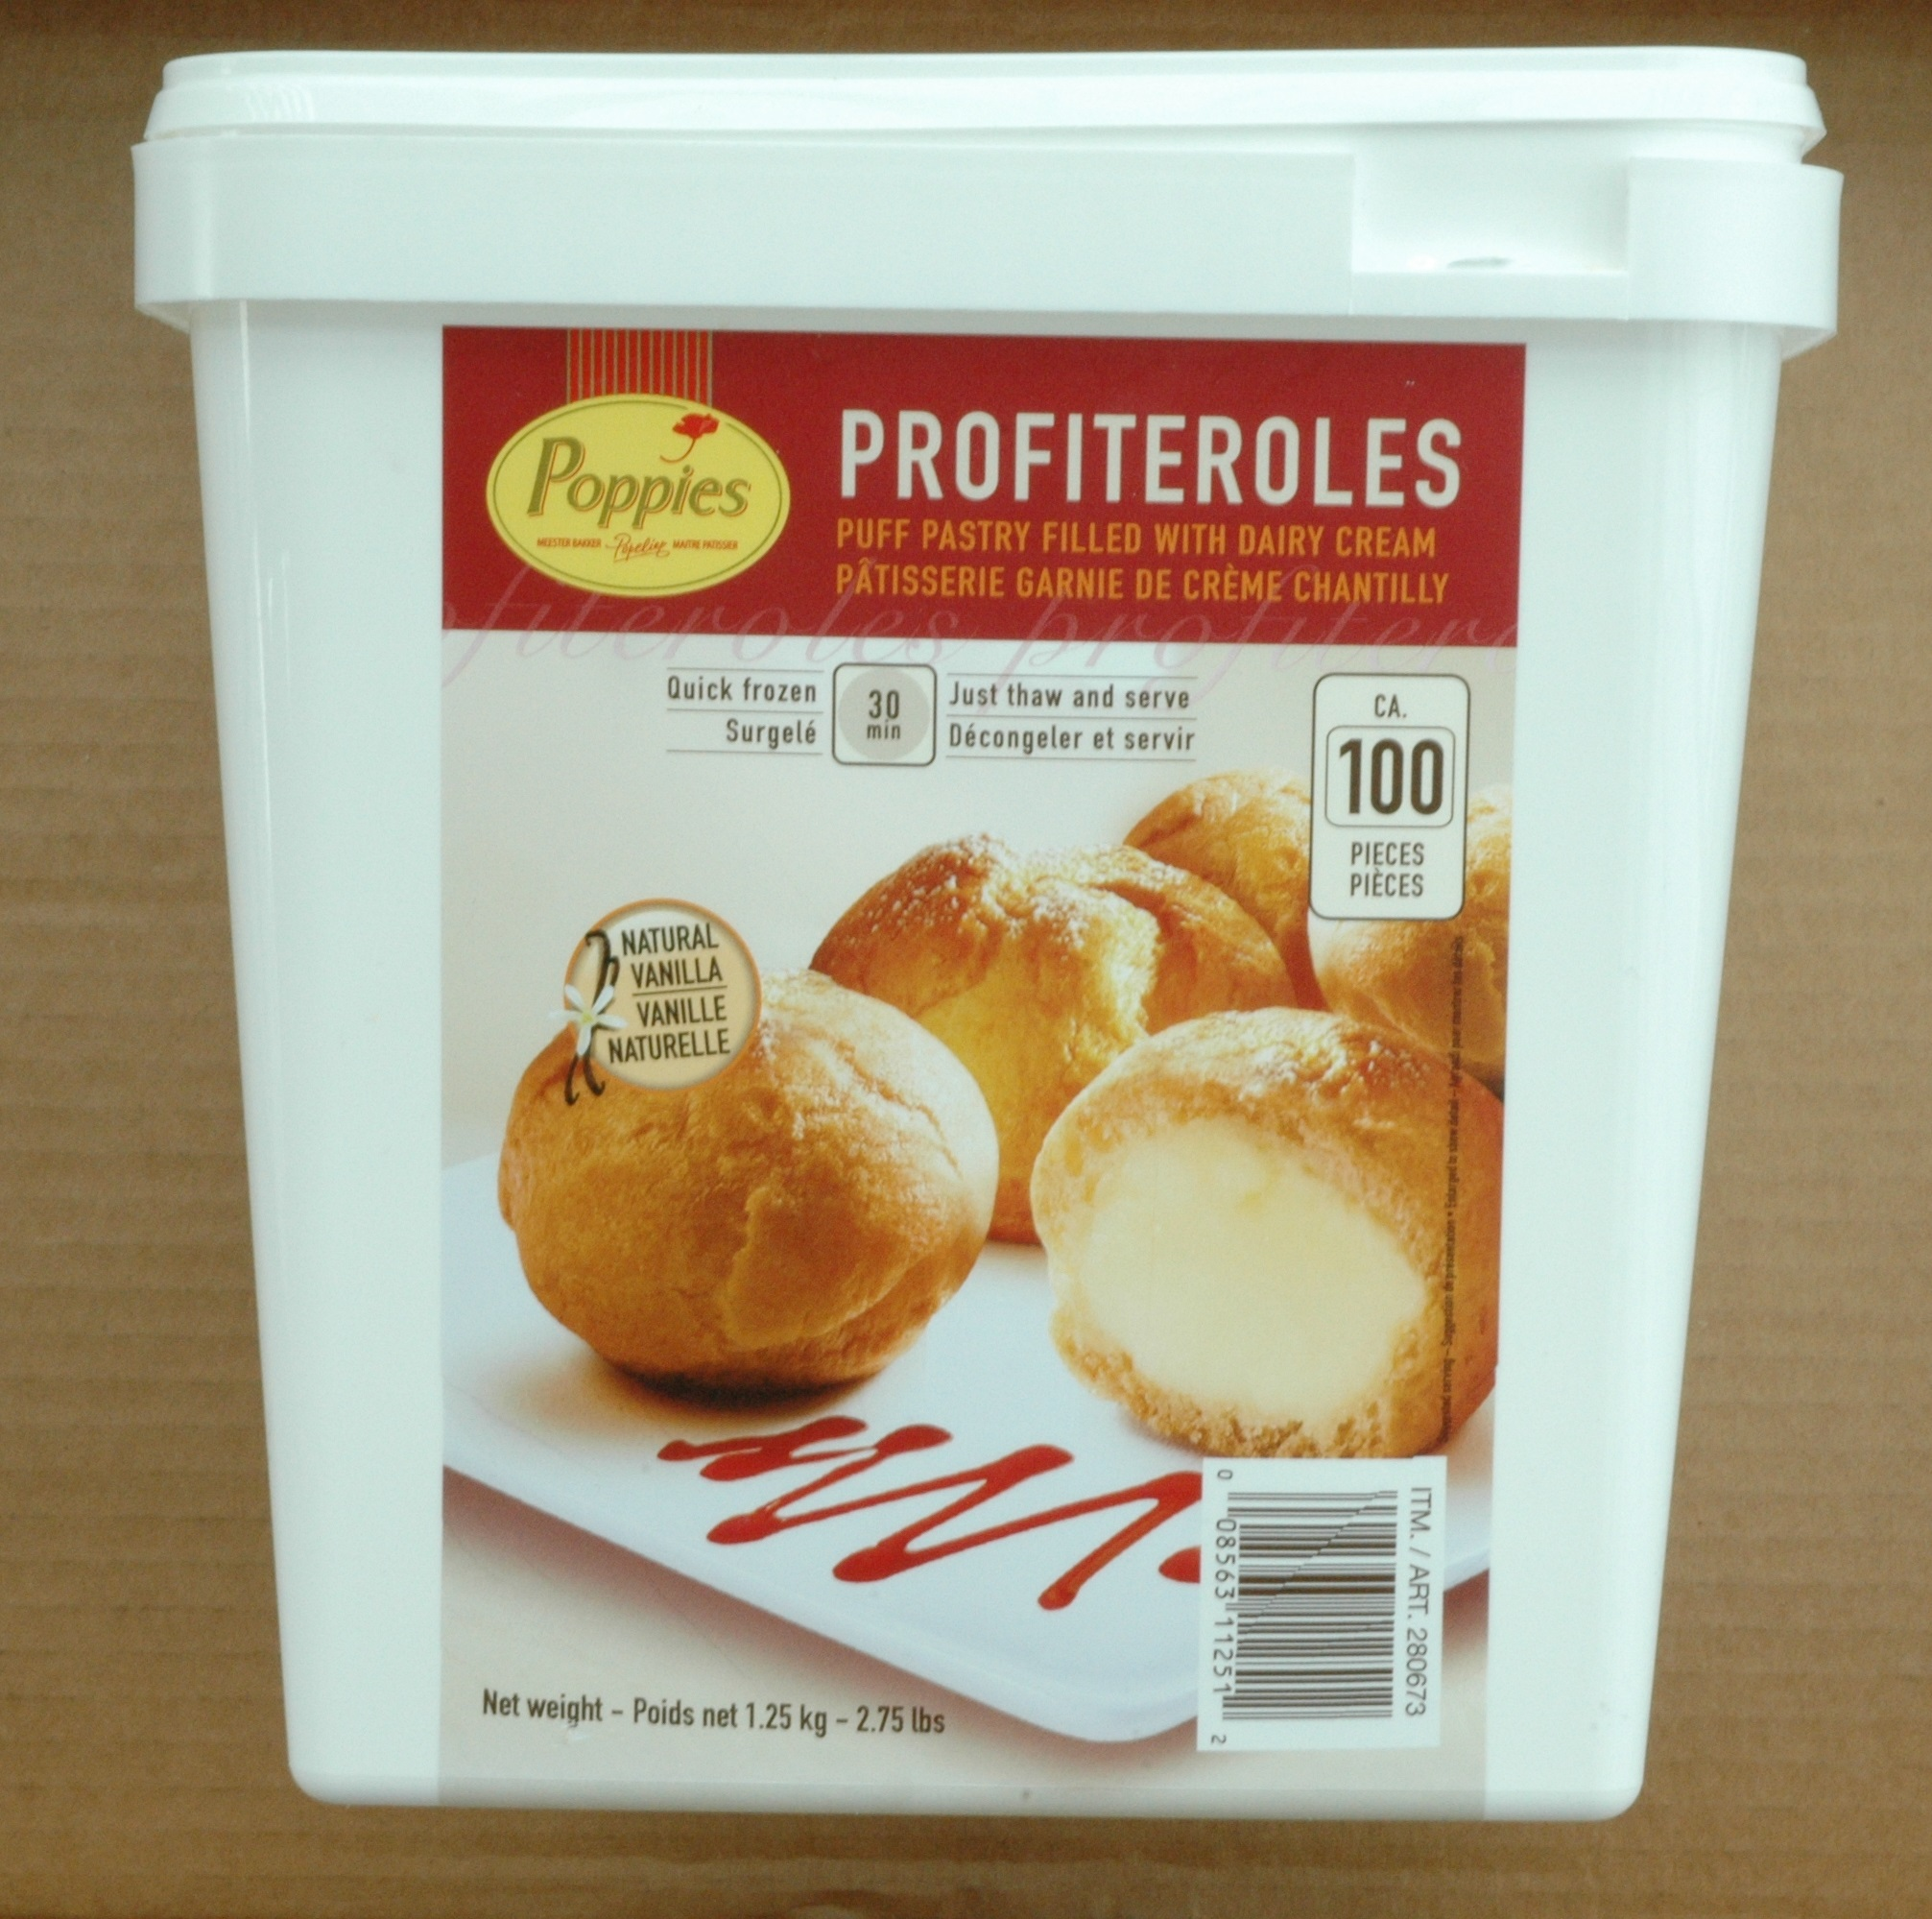
\includegraphics[width=0.3\textwidth]{interp/real_world_img/box/box} &
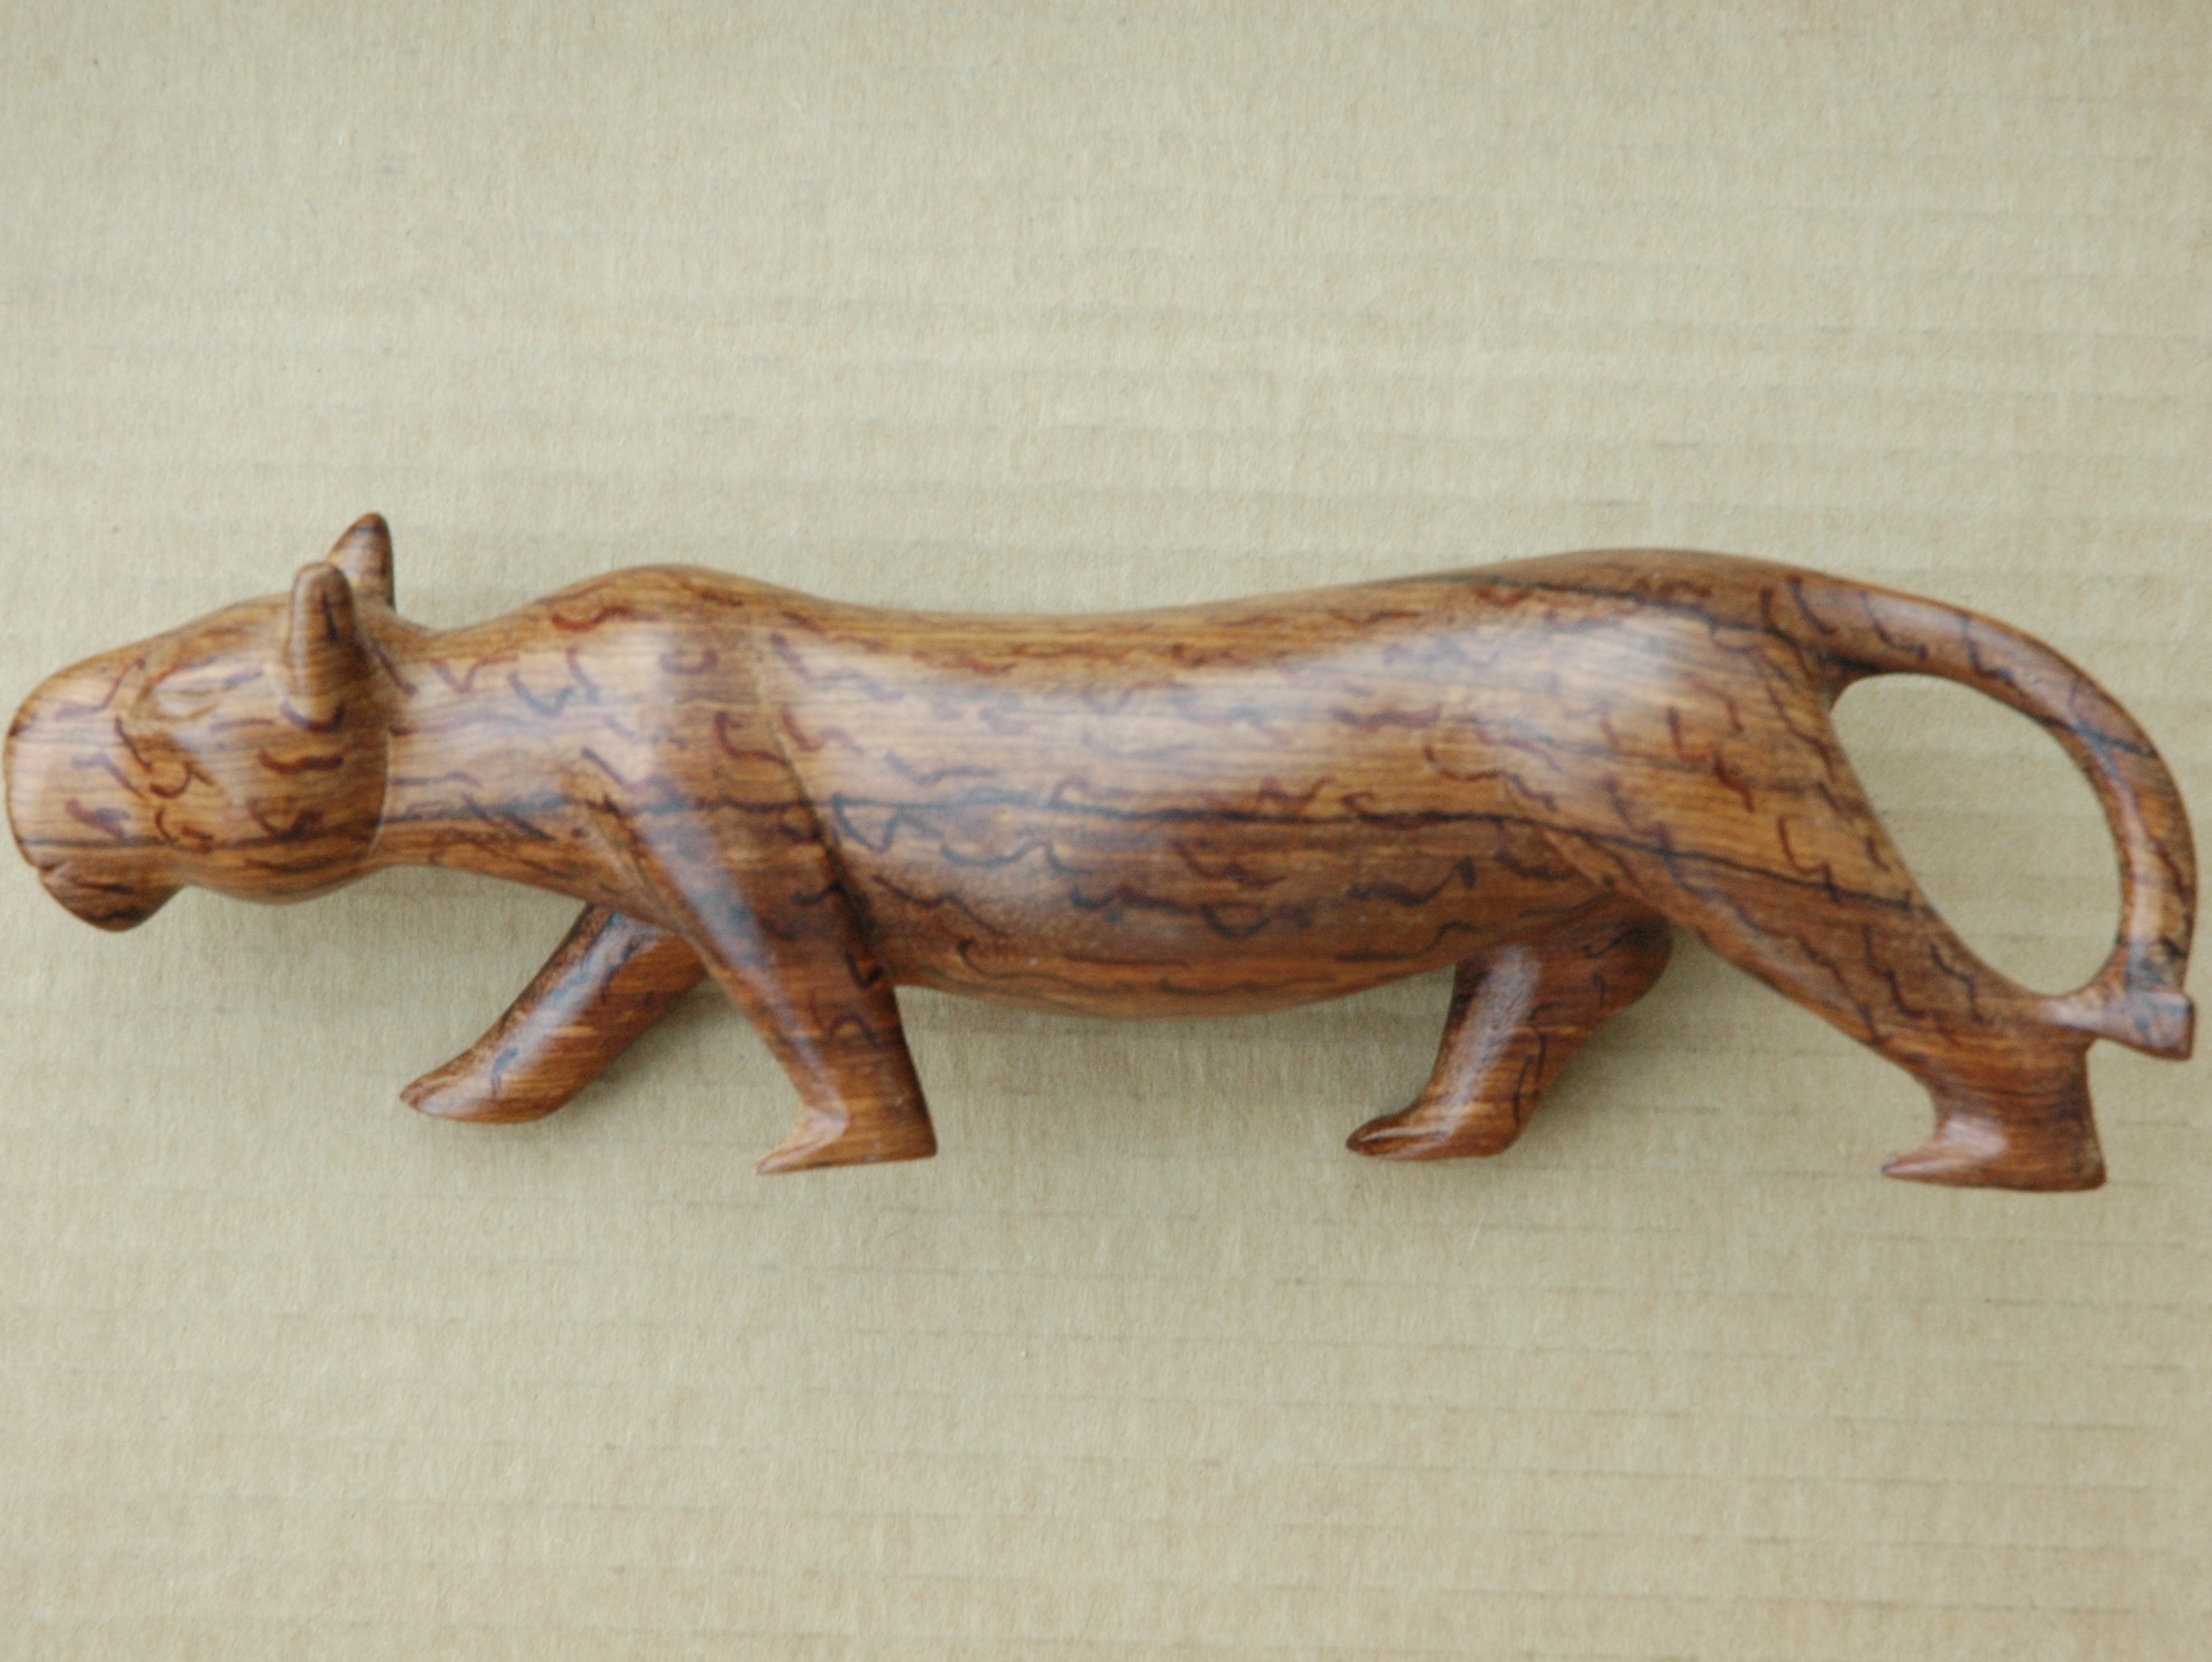
\includegraphics[width=0.3\textwidth]{interp/real_world_img/cat0/cat0} &
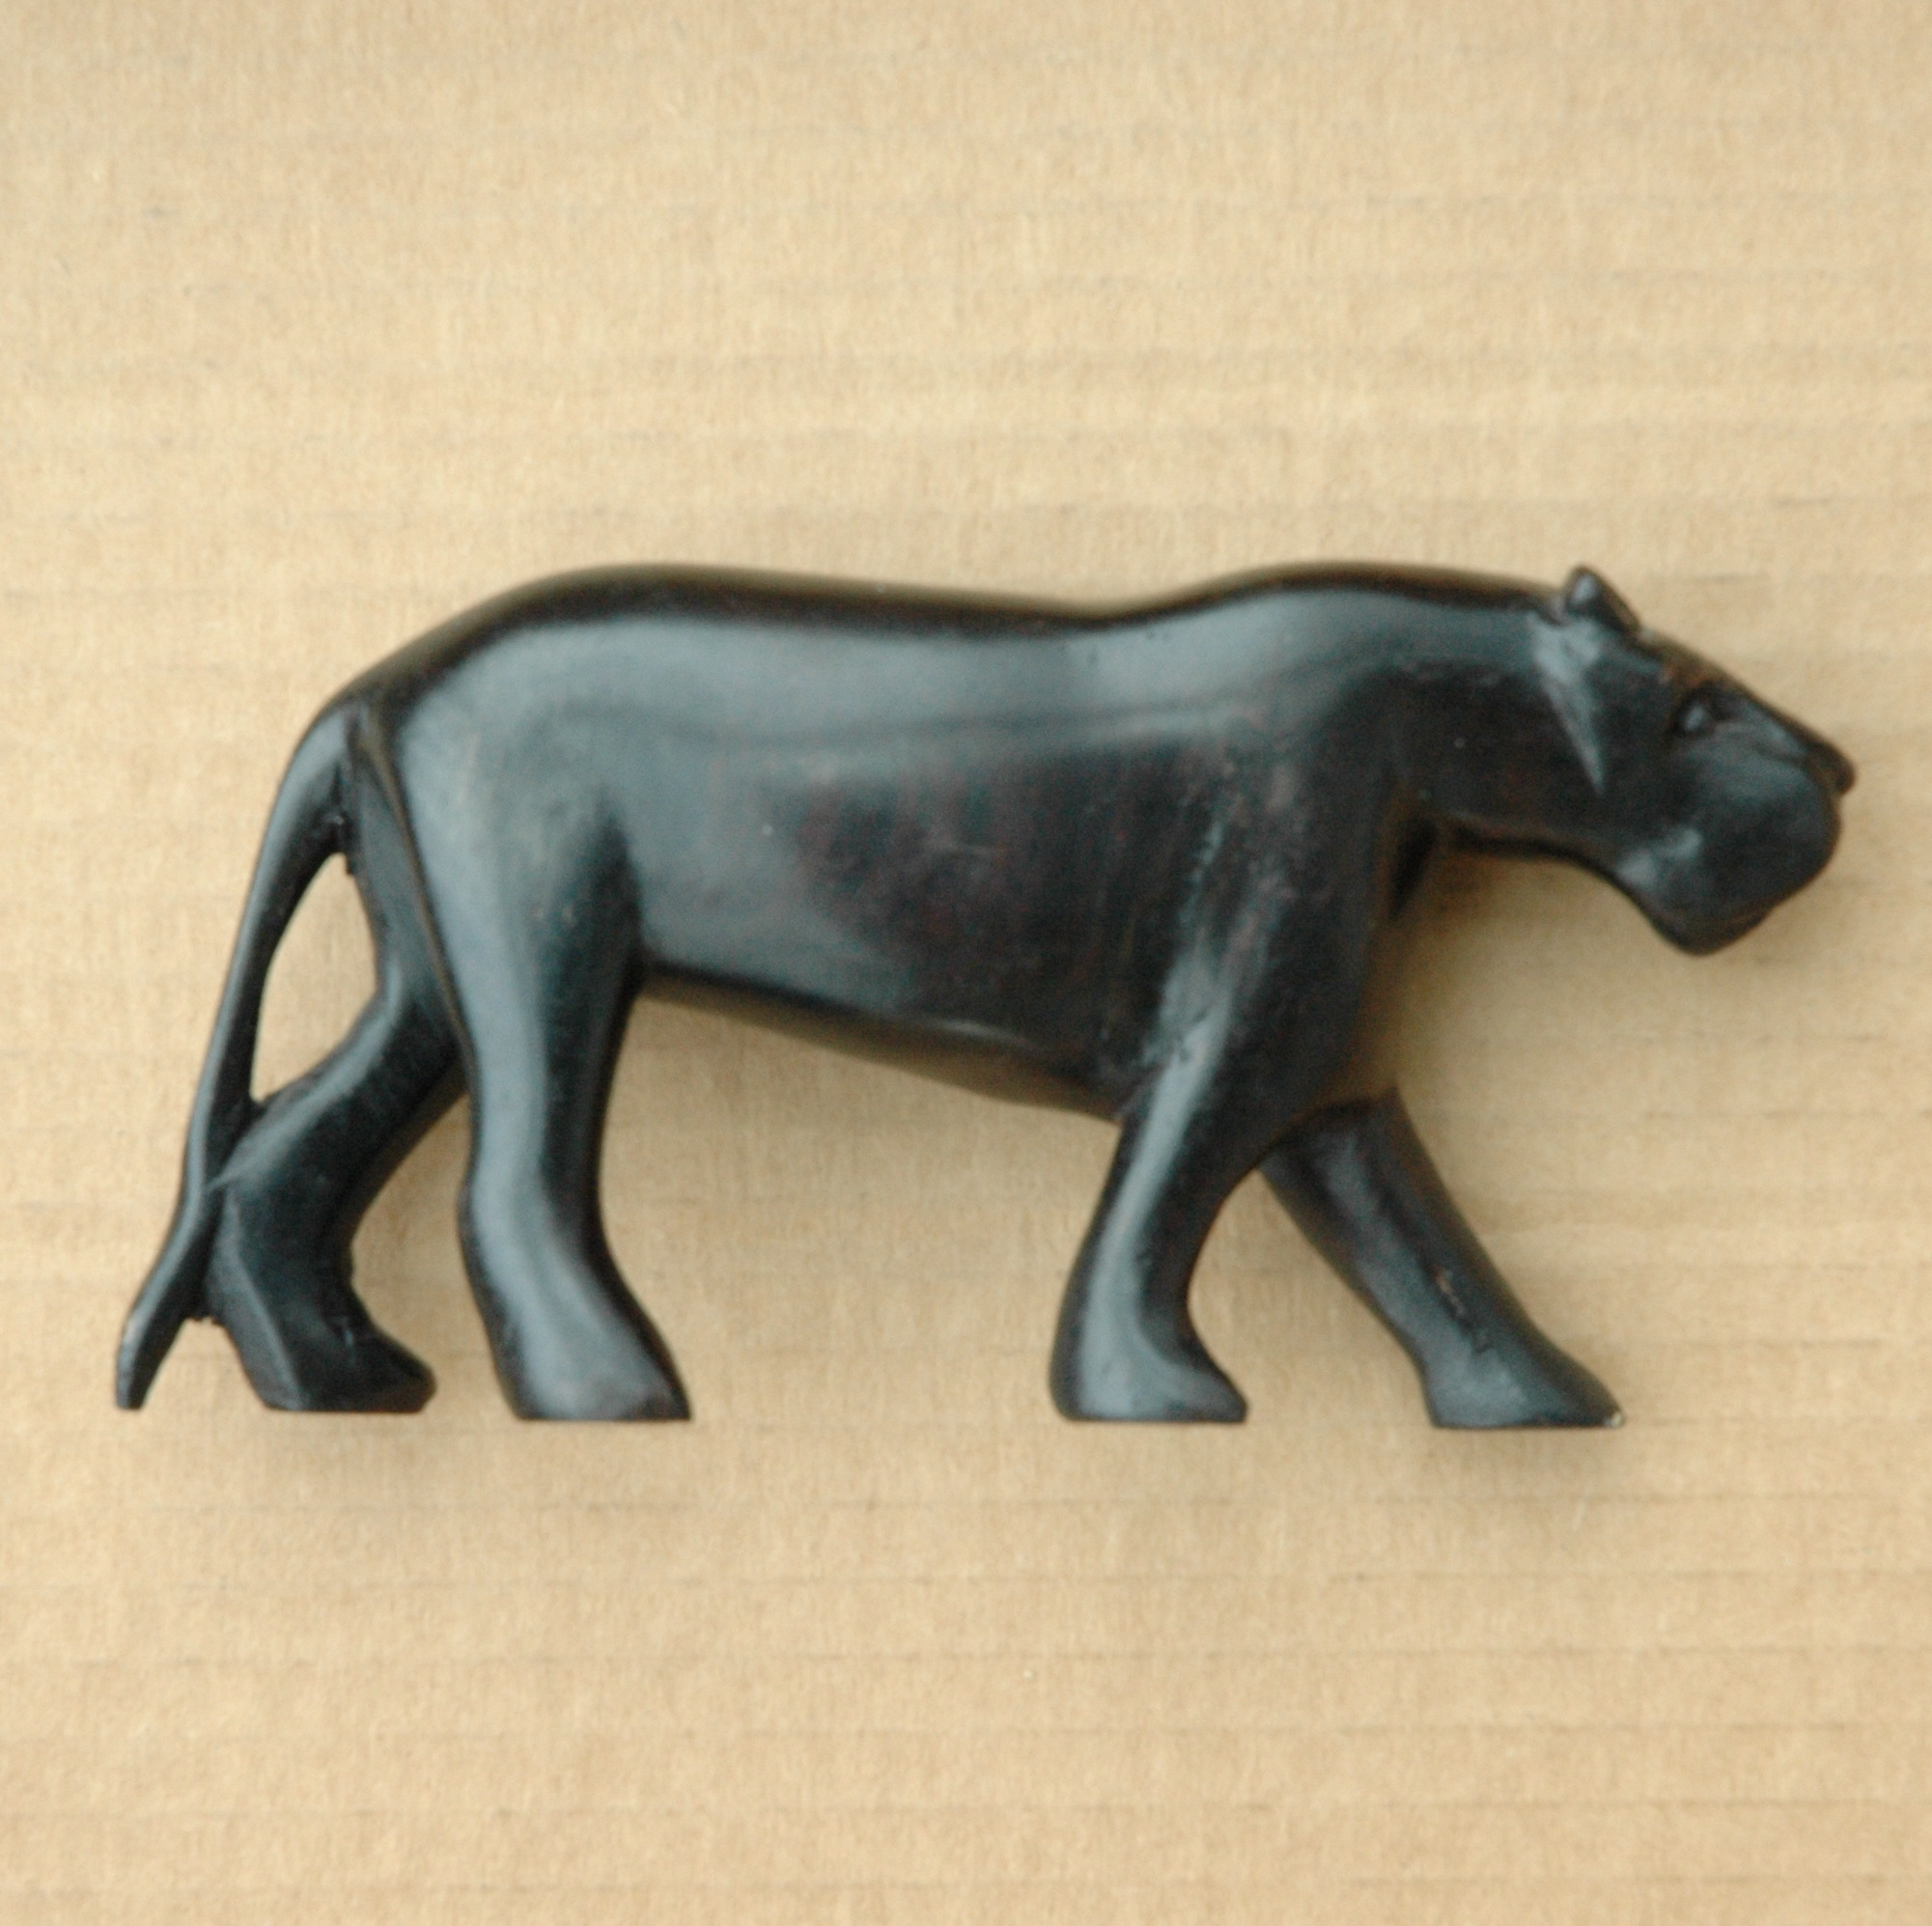
\includegraphics[width=0.3\textwidth]{interp/real_world_img/cat1/cat1} \\
(a). box & (b). cat0 & (c). cat1\\
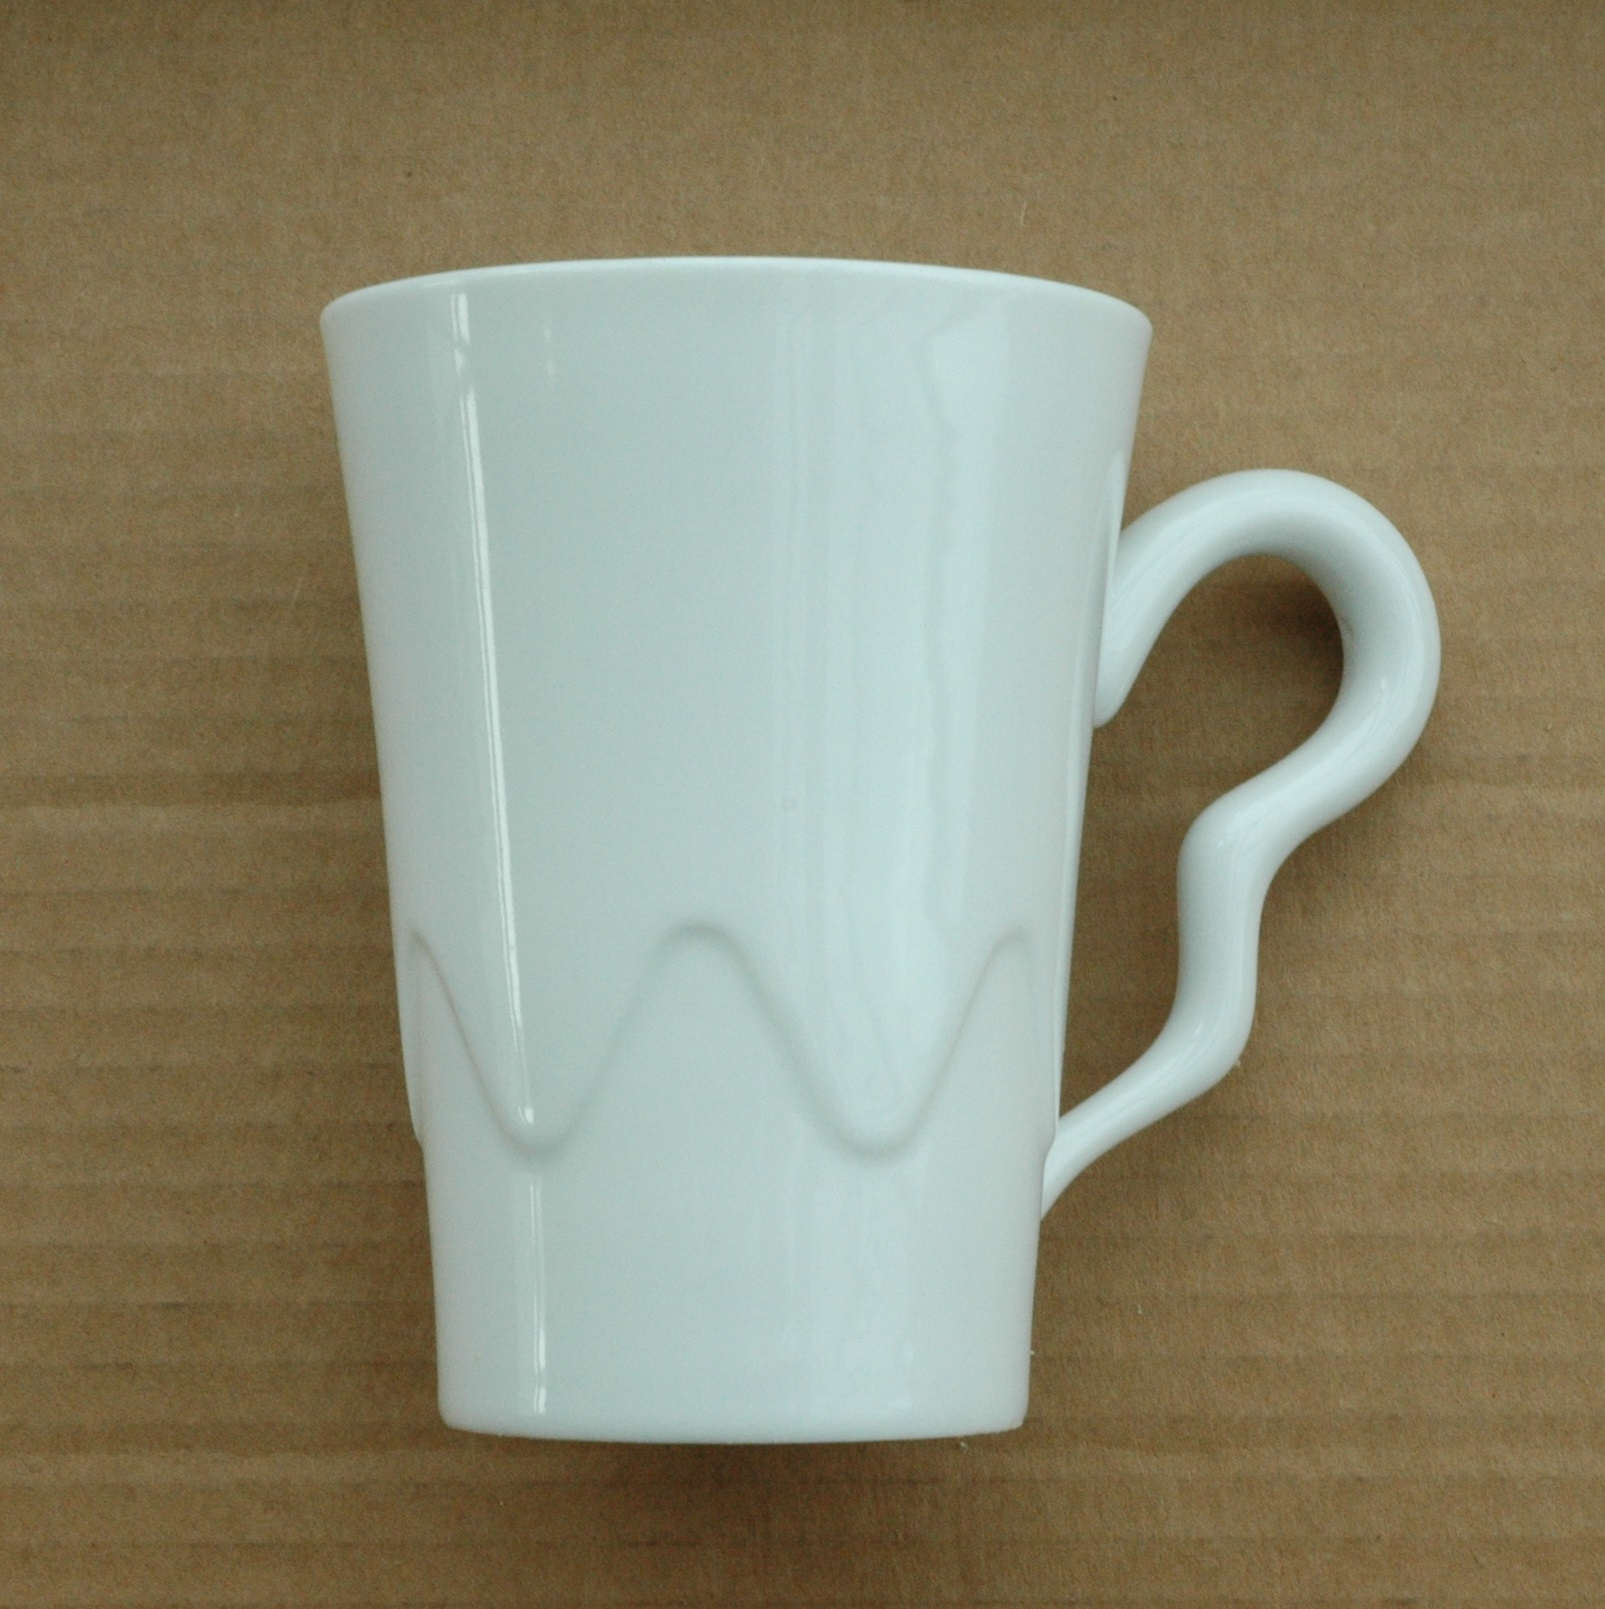
\includegraphics[width=0.3\textwidth]{interp/real_world_img/cup/cup} &
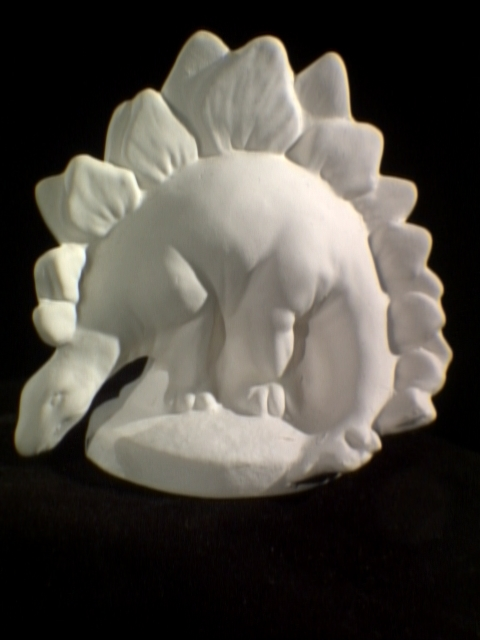
\includegraphics[width=0.3\textwidth]{interp/real_world_img/dino/dino} &
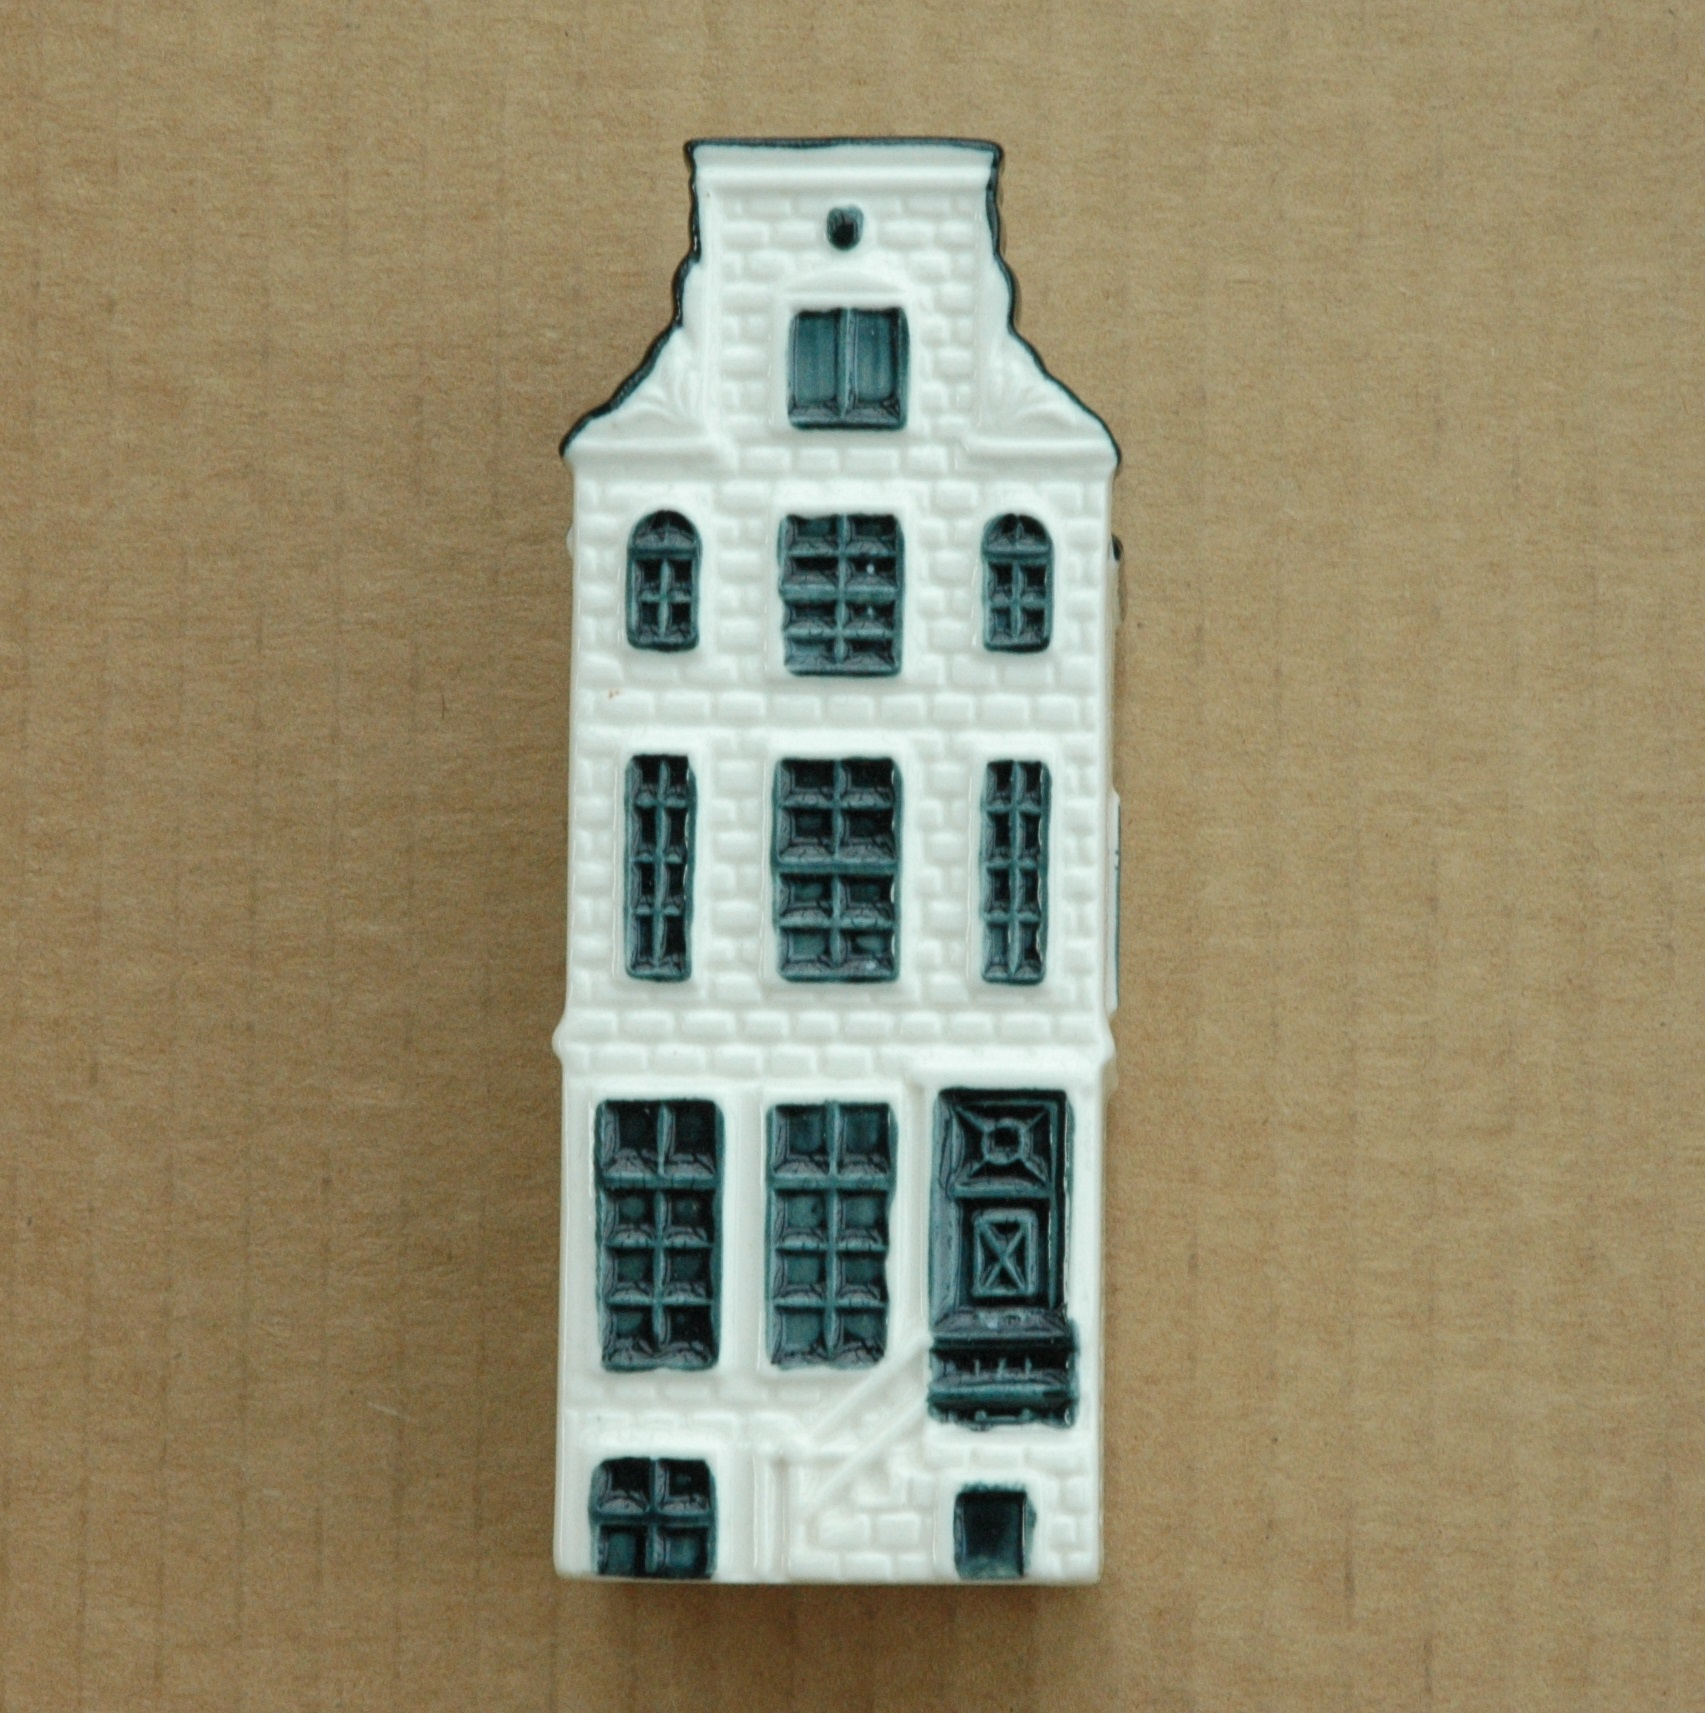
\includegraphics[width=0.3\textwidth]{interp/real_world_img/house/house}\\
(d). cup & (e). dino & (f). house\\
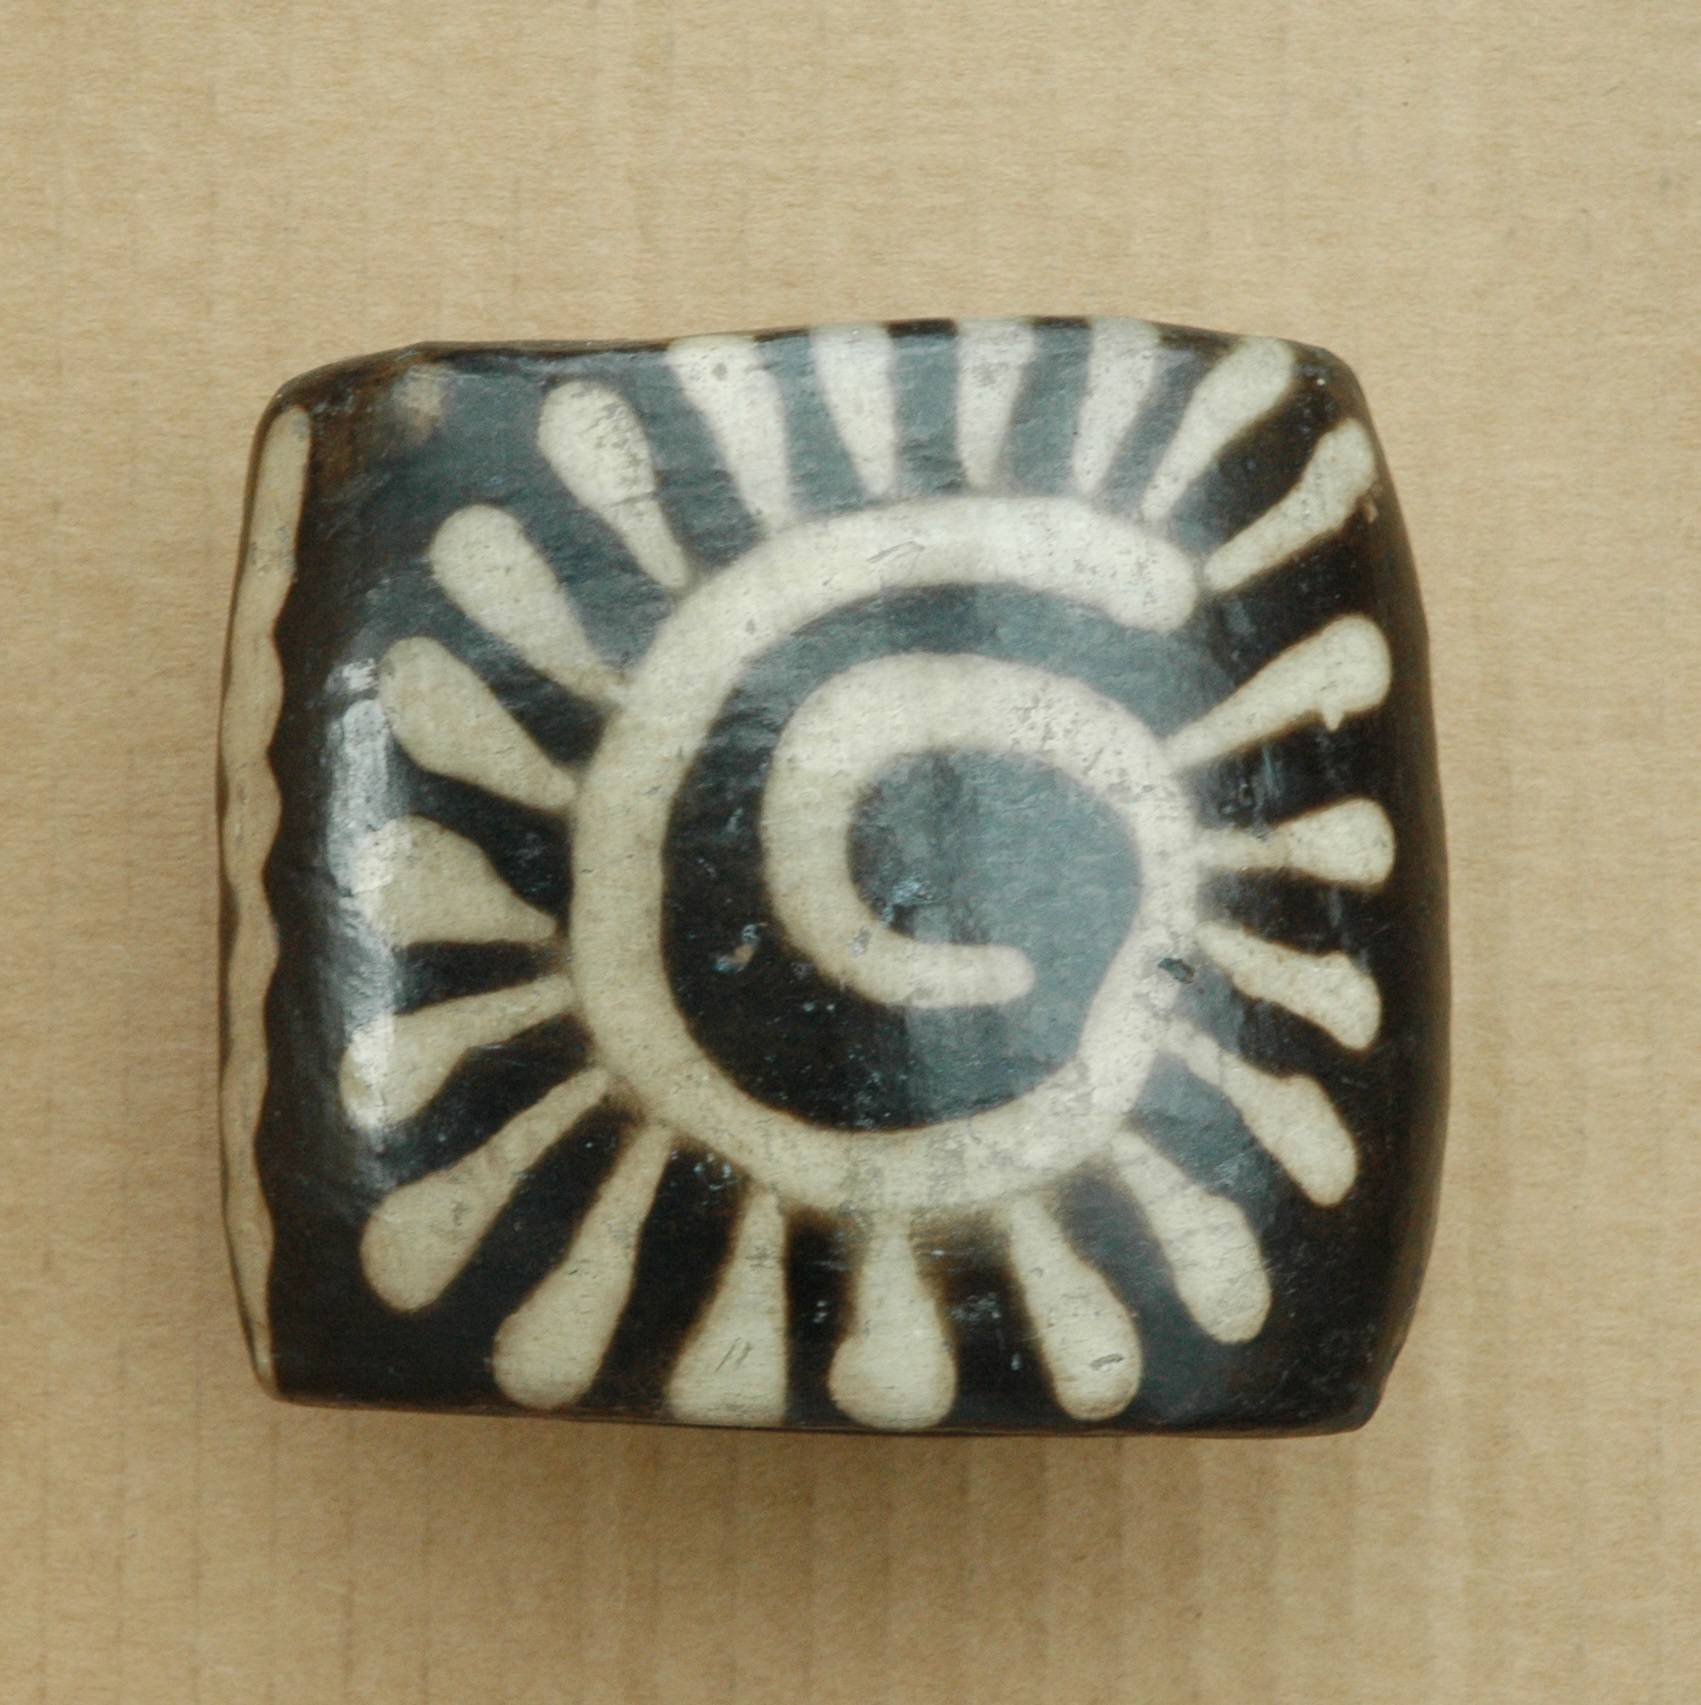
\includegraphics[width=0.3\textwidth]{interp/real_world_img/pot/pot} &
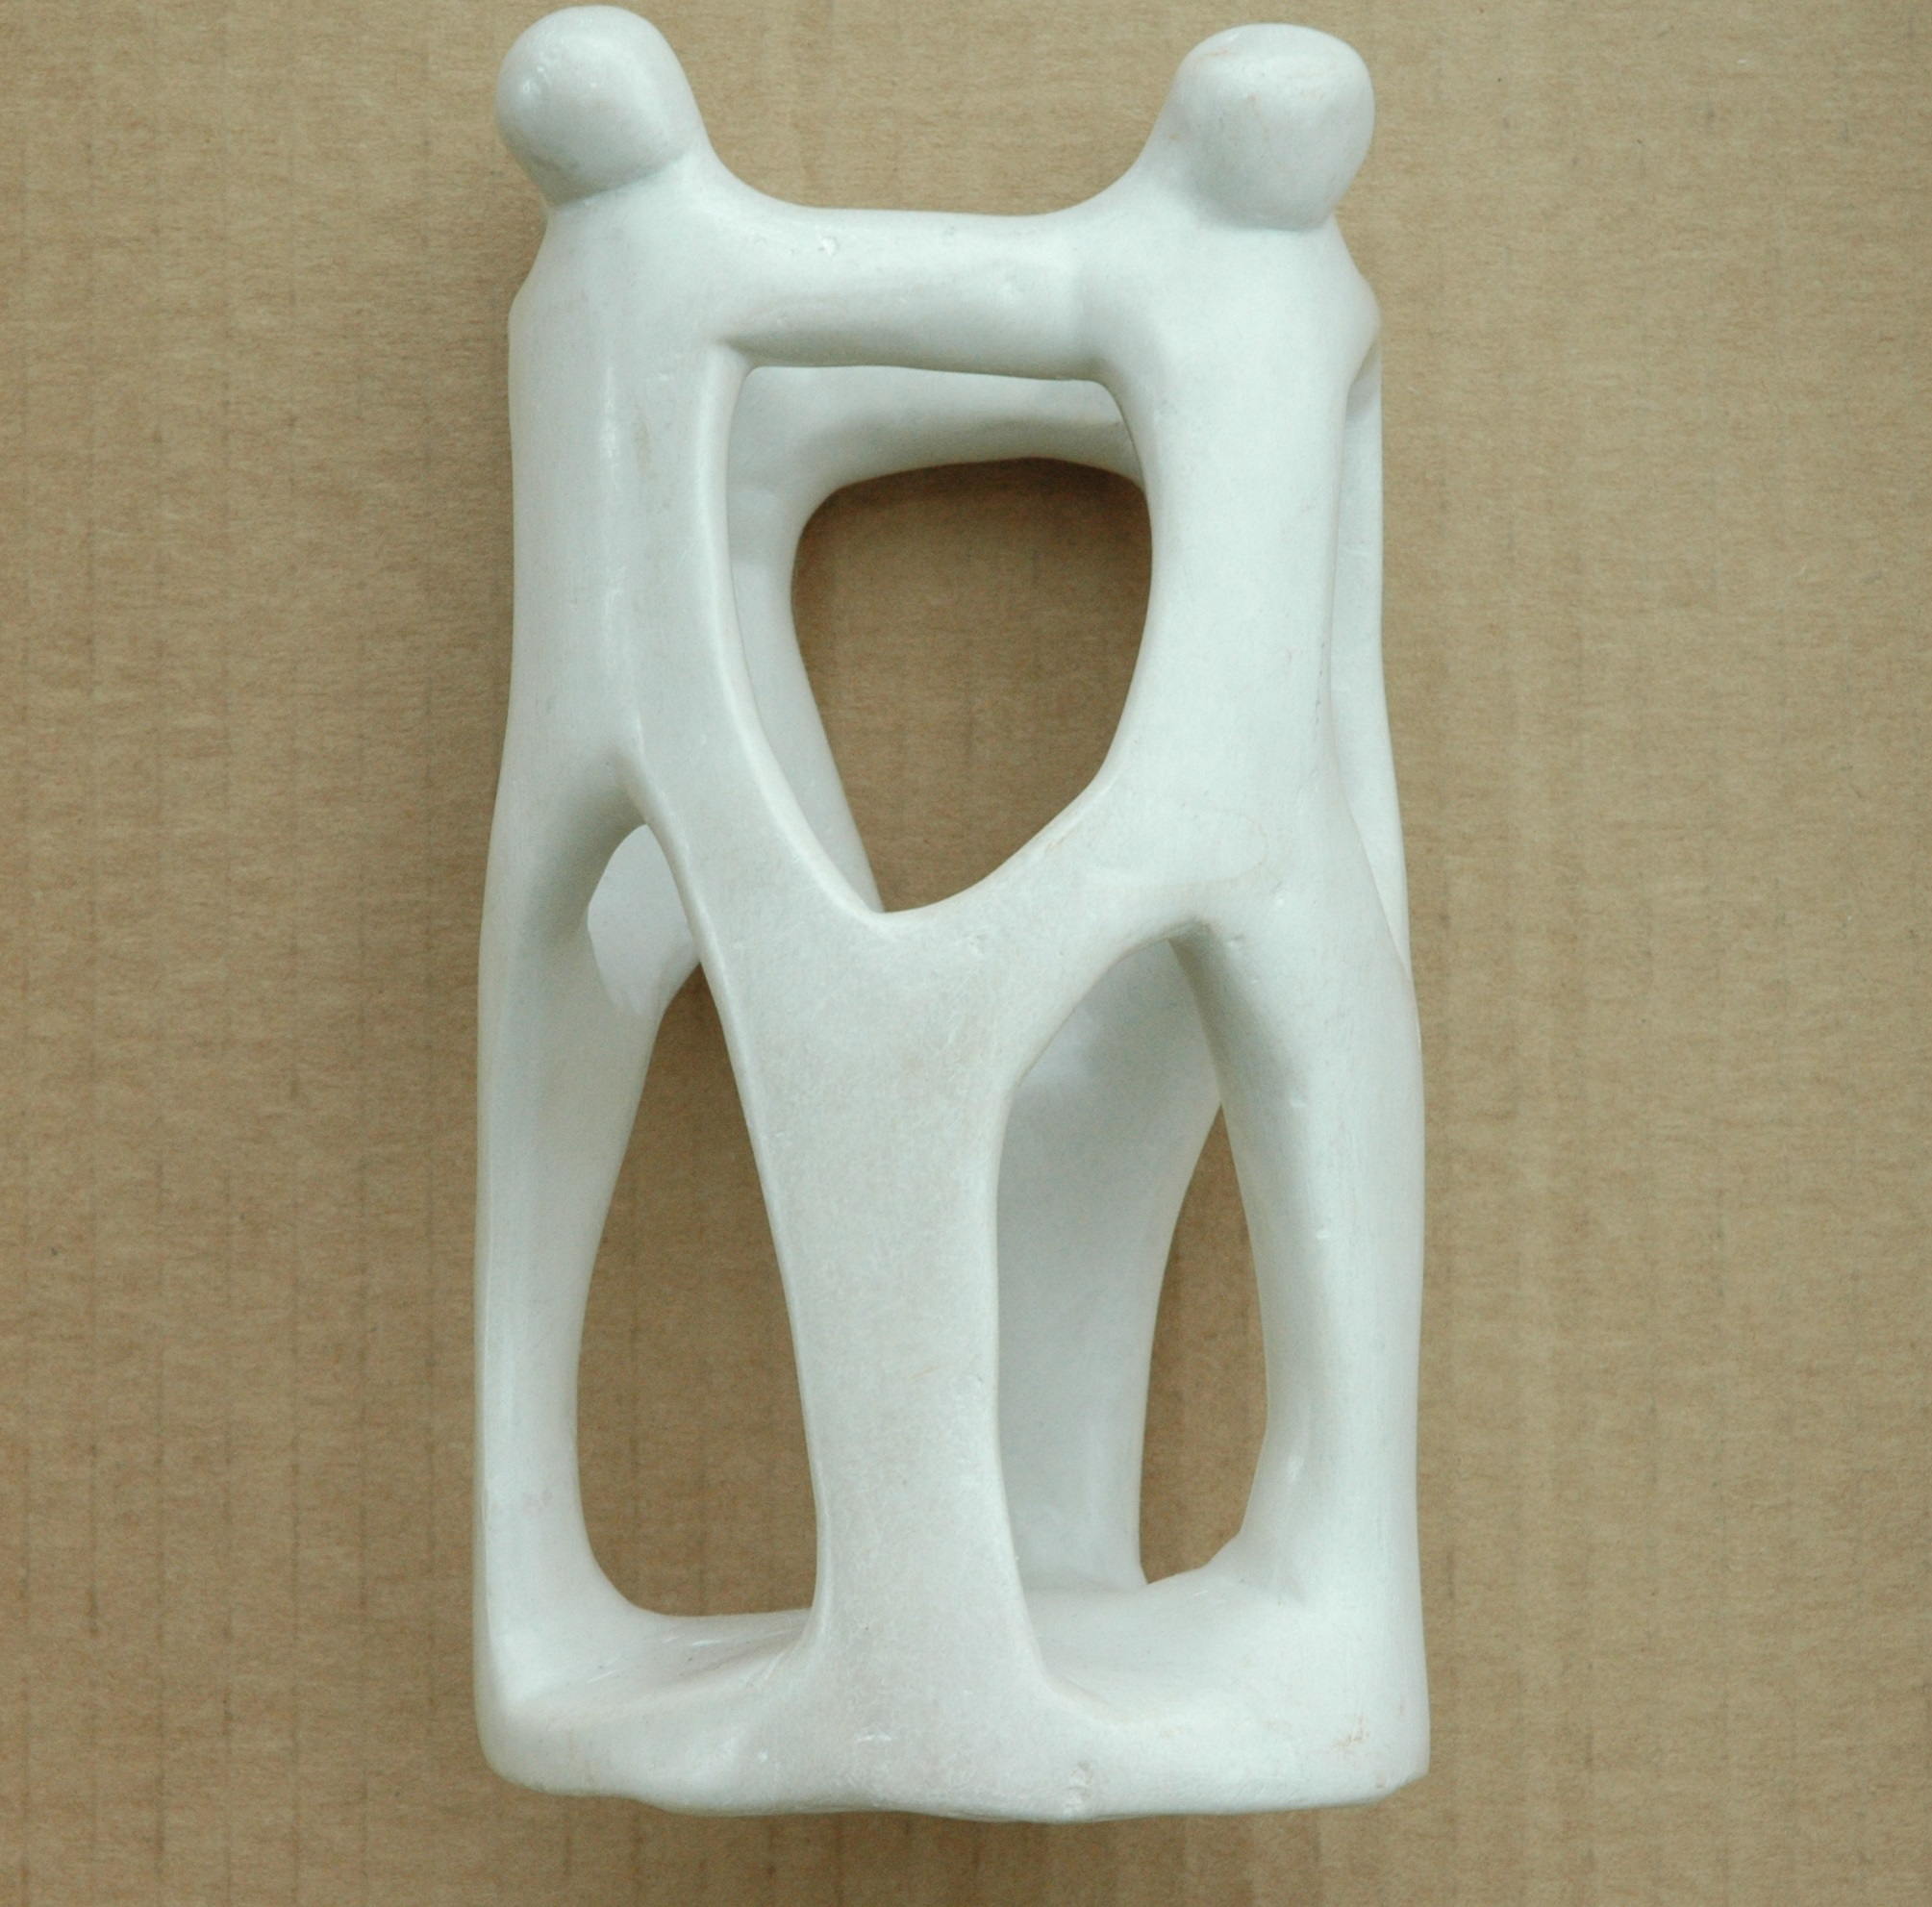
\includegraphics[width=0.3\textwidth]{interp/real_world_img/statue/statue} &
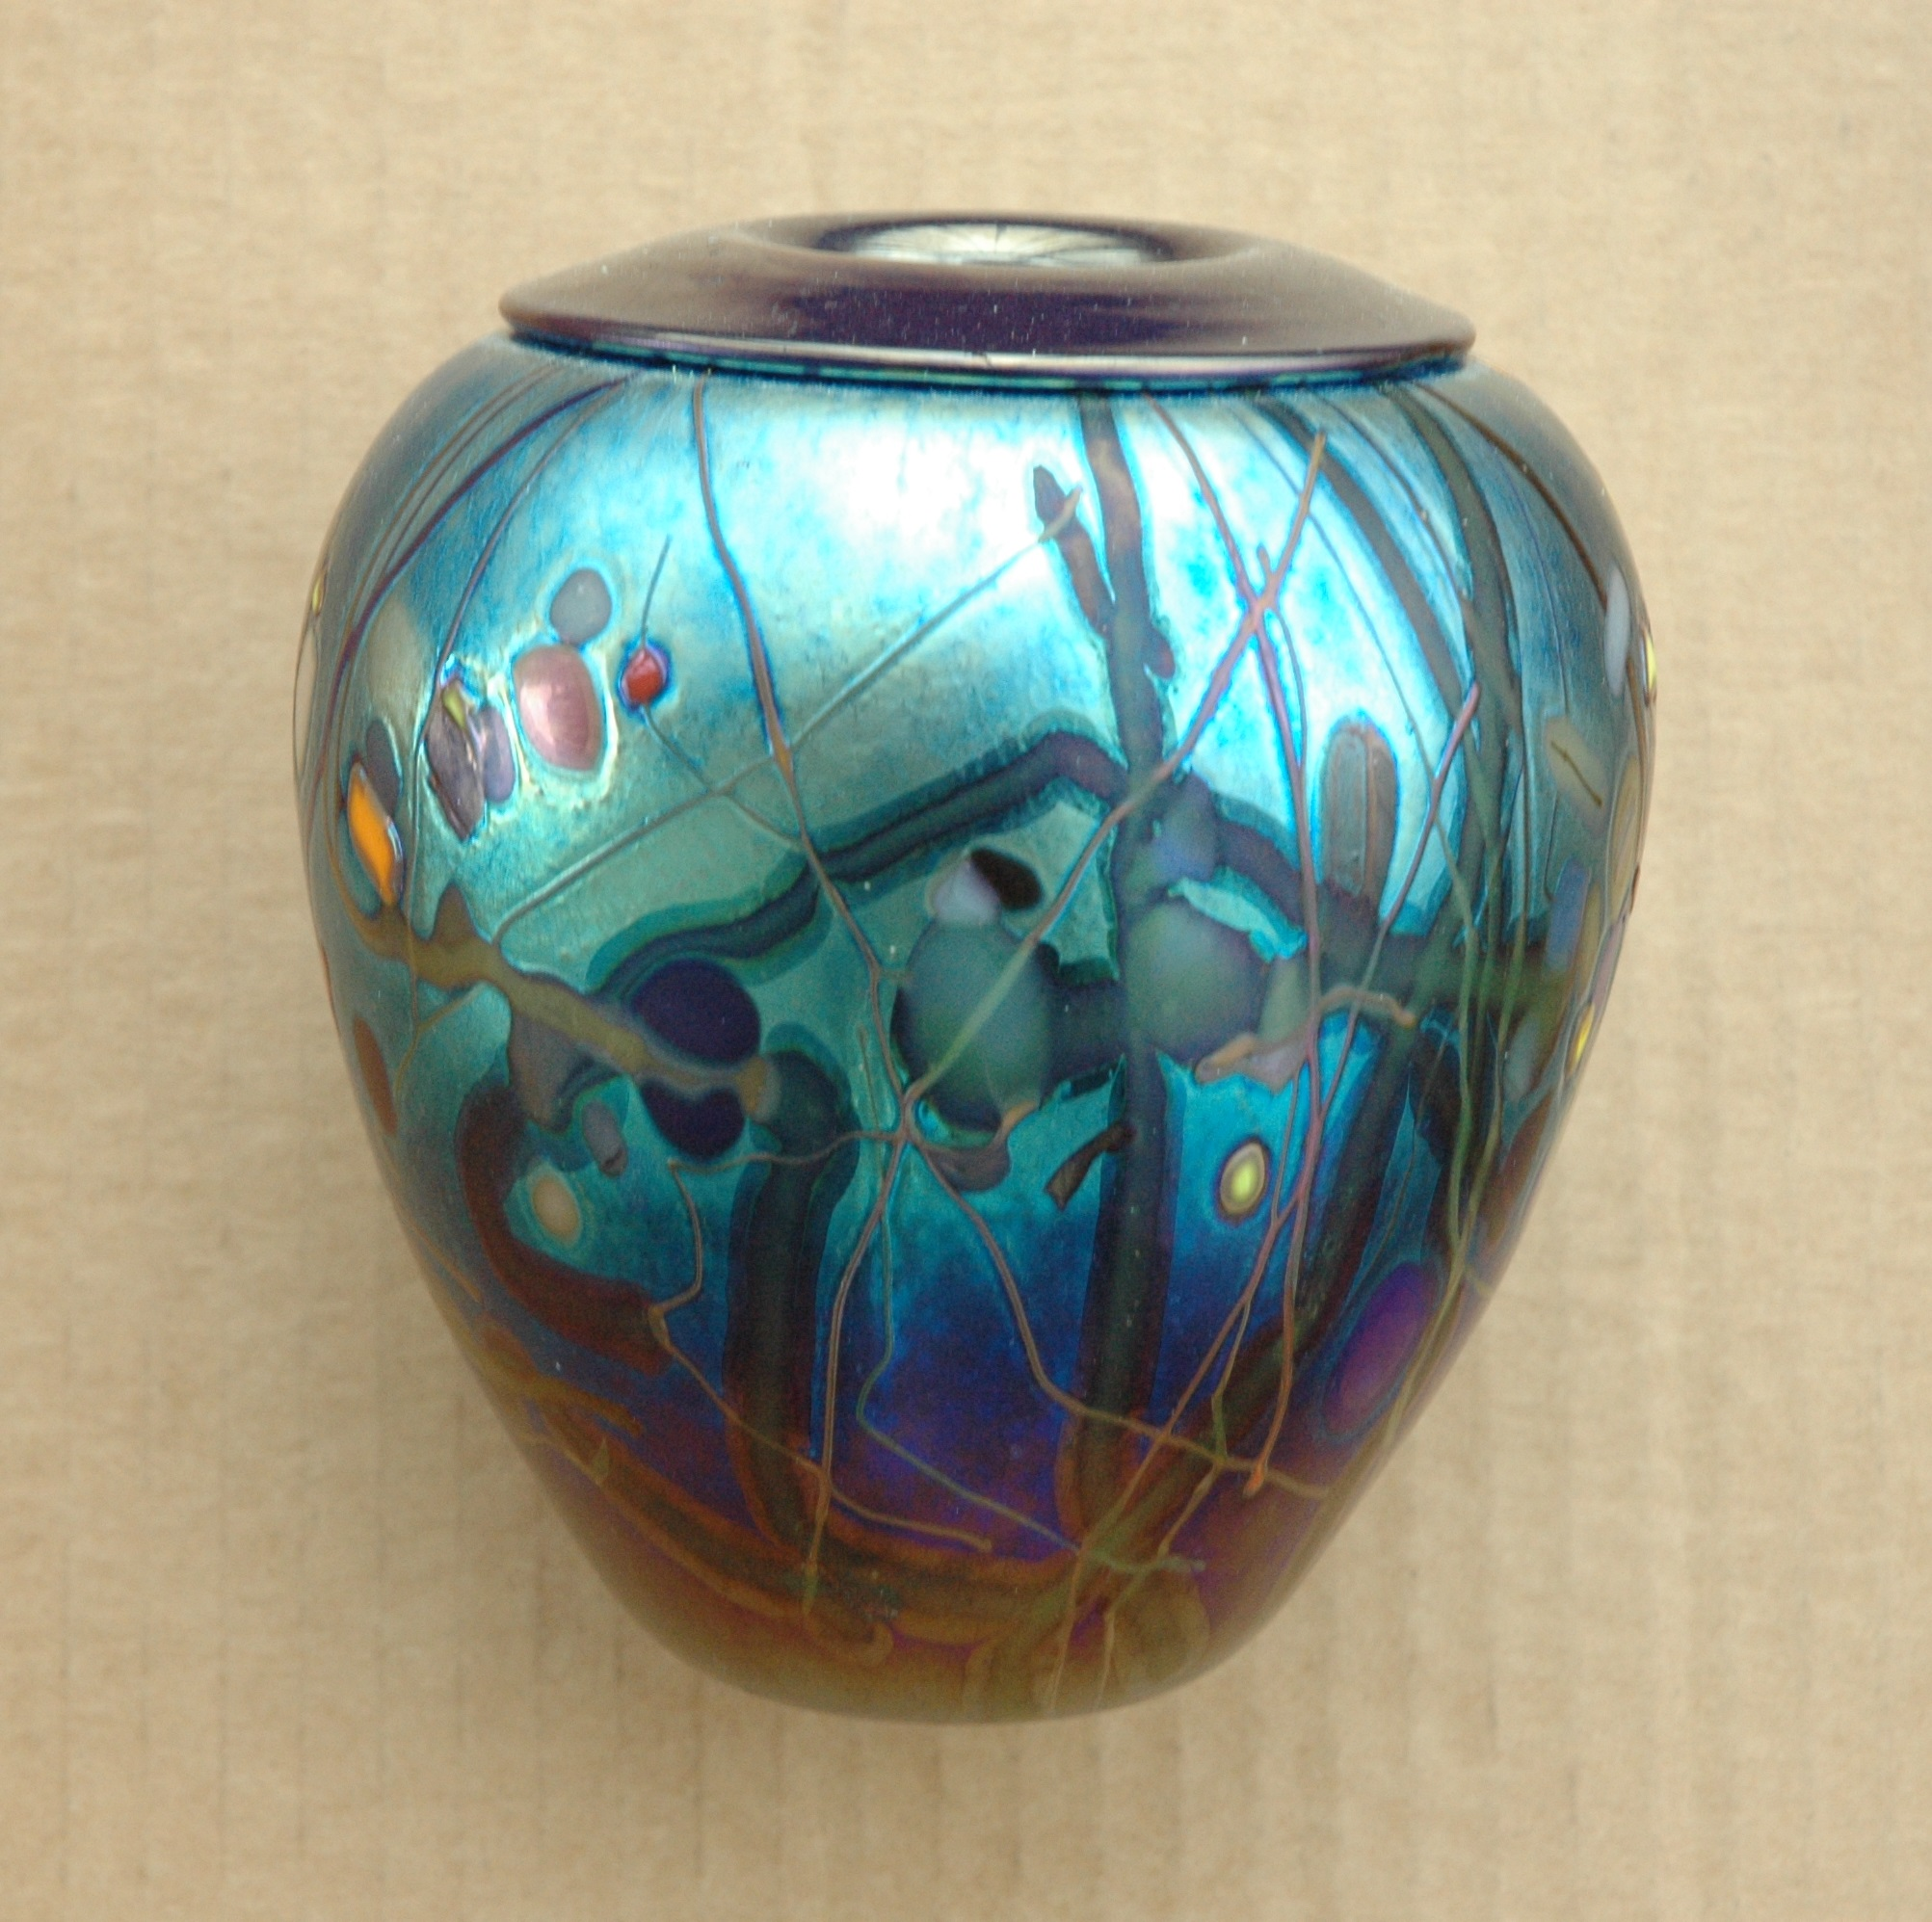
\includegraphics[width=0.3\textwidth]{interp/real_world_img/vase/vase} \\
(g). pot & (h). statue & (i). vase\\
\end{tabular}
\caption{Real-world dataset.}
\end{figure*}

\subsection{Data capture}
The images are captured using Nikon D70S camera with a $18-70mm$ lens. All images have a resolution of $3004\times 2000$. 

For MVS, we capture the dataset by positioning the camera in three different heights. The objects are about $30-50cm$ away from the camera, and is fixed on a turntable. We have followed the following three steps to acquire data: 1) put the camera at a different height, adjust the orientation so that the object in at the center of the frame; 2) take pictures while rotating the table. The table rotates approximately $30^\circ$ every time. We rotate it 12 times and in total, we can obtain 12 image per height.

For PS, a $70-200mm$ lens, a handheld lamp, and two reference objects (diffuse and glossy) are used. The objects are positioned about $3m$ from the camera to approximate orthographic projection. To avoid inter-reflection, all data are captured in a dark room with everying covered by black cloth except the target object. We use a hand-held lamp as the light source and choose close to frontal angle to avoid severe self-shadowing effect. We take 20 images per object and select 15 plus images depending on the severity of the self-shadow effect.

For SL, we use a Sanyo Pro xtraX Multiverse projector with a resolution of $1024\times 768$. The baseline angle is approximately $10^\circ$. To avoid the interference of ambient light, and inter-reflection, the objects are captured with room lights off.

\subsection{Calibration}
For MVS, a fixed random pattern is imaged with the object, which is used for camera calibration using SfM. The focal length is known and fixed, thus the extrinsic parameters of the camera can be retrieved up to a similarity transformation. Thus, the reconstruction is a metric/euclidean recontruction.

For SL, a opensource calibration software developed by~\citeauthor{moreno2012simple} is used for camera-projector calibration. This technique works by projecting temporal patterns on the object, and uses local homography to individually translate each checkerboard corner from the camera plane to the projector plane.

\section{Evaluation of Interpreter}
\label{sec:eval_interp}
This section evaluates the proof of concept interpreter, which should return a successful result given a valid description, or a less successful one given an incorrect description. We choose four different problem conditions where each describes one of the four major classes of objects and provides demonstrative results.

\subsection{Synthetic Datasets}
We generate a dataset of four objects, each representing one of the four classes discussed in Section~\ref{ch:3DRecon_Taxo}. The mapping from problem conditions to algorithms are summarized in Table~\ref{tab:synth_prop_list}. Given a specific algorihthm, the proof-of-concept interpreter will select an algorithm, and any object that matches this description should be well reconstructed by this algorithm. We use four descriptions that match the four problem conditions listed in Table so that each object should at least return one well reconstructed result. Since a problem condition could be mapped to multiple algorithms, an object that does not match the description could potentially have a satisfactory result as well. The reconstruction results of test objects and those of the baseline method are shown in Figure~\ref{fig:synth_results}.
\begin{table}[!htbp]
  \centering
  \begin{tabular}{lllllll}
  \hline
  \textbf{C\#} & \textbf{Object} & Texture & Albedo & Specular & Rough & Mapping\\
  \hline
  1 & bust & 0.2 & 0.8 & 0.2 & 0.8 & EPS, GSL\\
  2 & vase1 & 0.2 & 0.8 & 0.8 & 0.2 & EPS\\
  3 & barrel & 0.8 & 0.8 & 0.2 & 0.8 & PMVS, EPS, GSL\\
  4 & vase0 & 0.8 & 0.8 & 0.8 & 0.2 & PMVS , EPS\\
  \hline
  \end{tabular}
  \caption{Problem conditions and mapping of the synthetic objects.}
  \label{tab:synth_prop_list}
\end{table}

\begin{figure*}[!htbp]
\centering
\begin{tabular}{lccccr}
\toprule
Desc \# & Bust & Vase1 & Barrel & Vase0 & Selected Algo.\\
\midrule
1 & 
\fcolorbox{green}{white}{\raisebox{-.5\height}{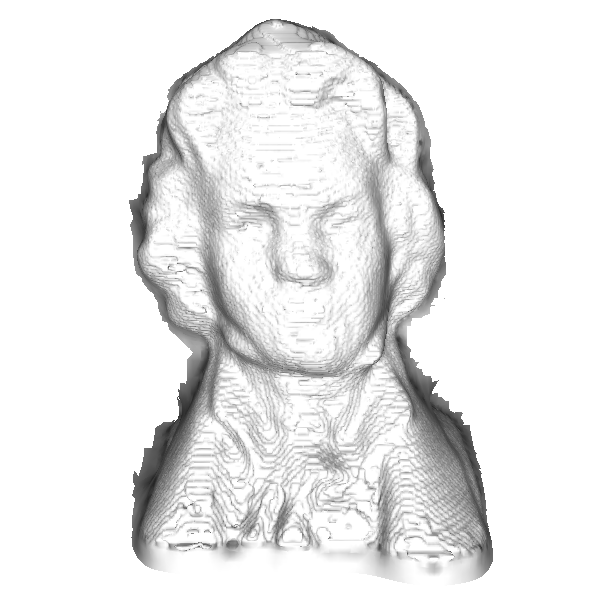
\includegraphics[width=0.1\textwidth]{interp/synth_interp/beethoven_sl}}}&
\raisebox{-.5\height}{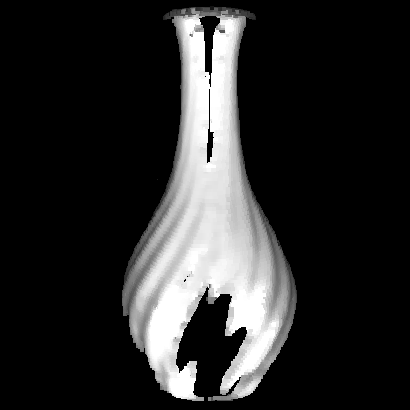
\includegraphics[width=0.1\textwidth]{interp/synth_interp/vase0_sl}}&
\raisebox{-.5\height}{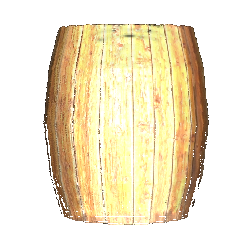
\includegraphics[width=0.1\textwidth]{interp/synth_interp/barrel_sl}}&
\raisebox{-.5\height}{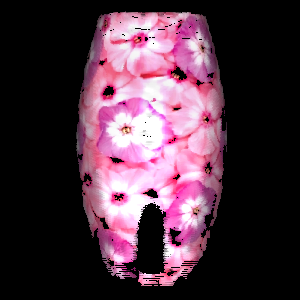
\includegraphics[width=0.1\textwidth]{interp/synth_interp/vase2_sl}}&
GSL\\
2 & 
\raisebox{-.5\height}{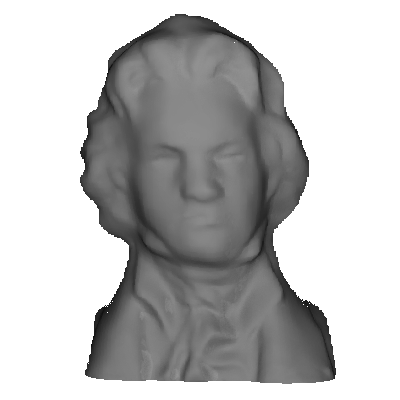
\includegraphics[width=0.1\textwidth]{interp/synth_interp/beethoven_ps}}&
\fcolorbox{green}{white}{\raisebox{-.5\height}{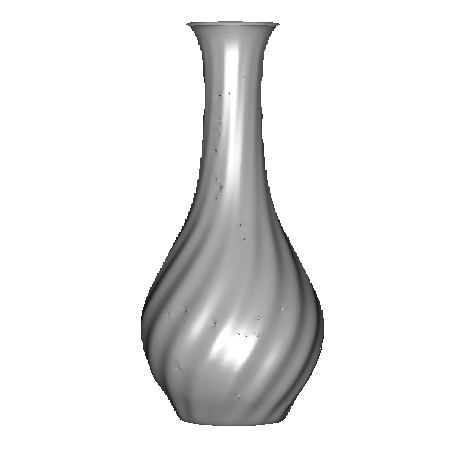
\includegraphics[width=0.1\textwidth]{interp/synth_interp/vase0_ps}}}&
\raisebox{-.5\height}{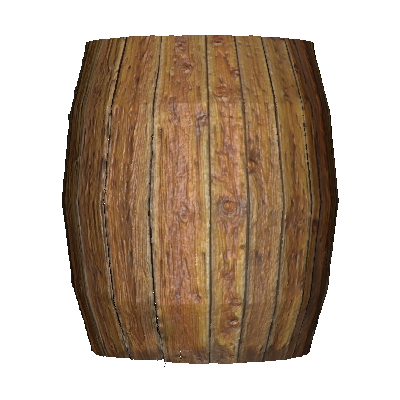
\includegraphics[width=0.1\textwidth]{interp/synth_interp/barrel_ps}}&
\raisebox{-.5\height}{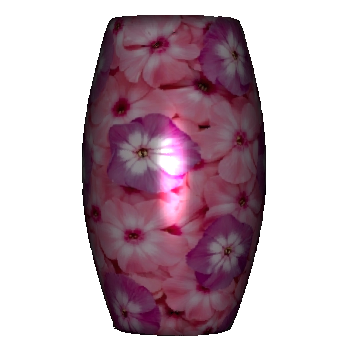
\includegraphics[width=0.1\textwidth]{interp/synth_interp/vase2_ps}}&
EPS\\
3 & 
\raisebox{-.5\height}{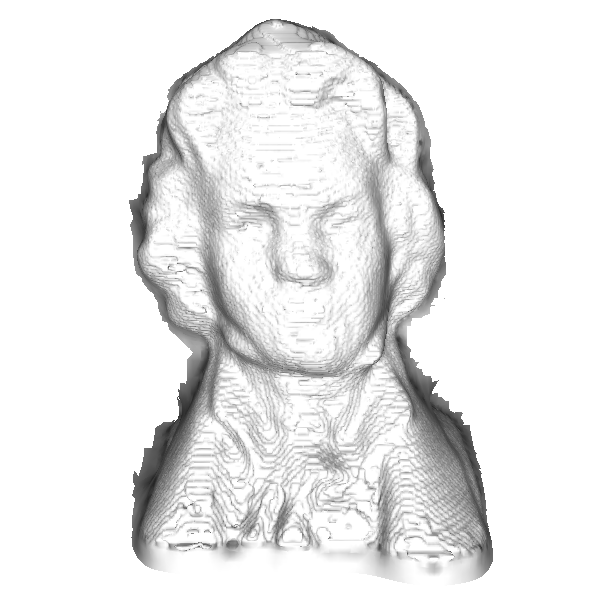
\includegraphics[width=0.1\textwidth]{interp/synth_interp/beethoven_sl}}&
\raisebox{-.5\height}{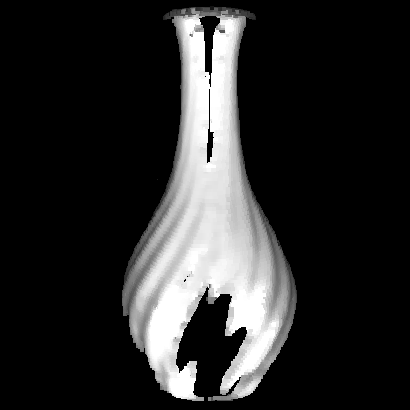
\includegraphics[width=0.1\textwidth]{interp/synth_interp/vase0_sl}}&
\fcolorbox{green}{white}{\raisebox{-.5\height}{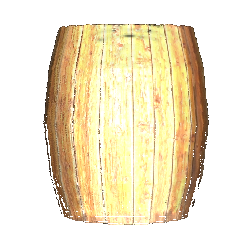
\includegraphics[width=0.1\textwidth]{interp/synth_interp/barrel_sl}}}&
\raisebox{-.5\height}{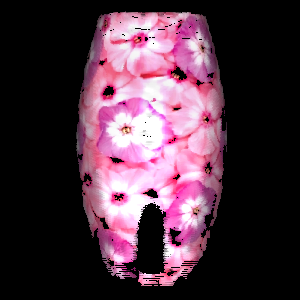
\includegraphics[width=0.1\textwidth]{interp/synth_interp/vase2_sl}}&
GSL\\
4 &
\raisebox{-.5\height}{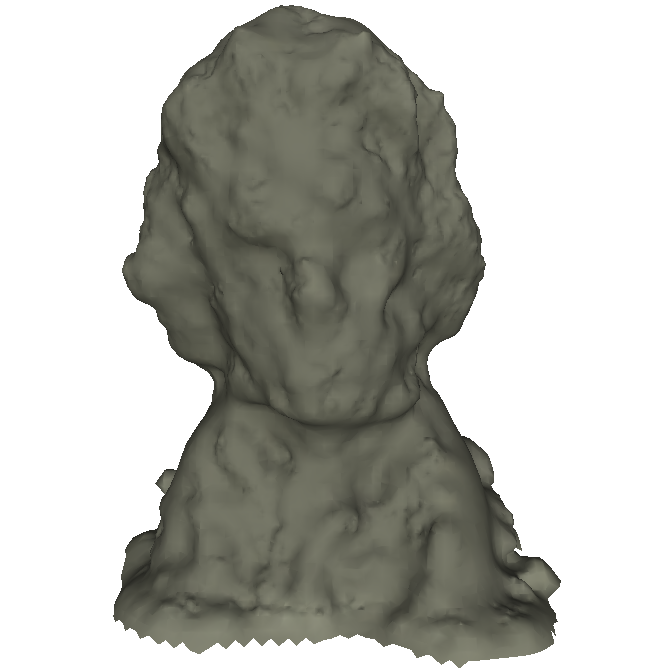
\includegraphics[width=0.1\textwidth]{interp/synth_interp/beethoven_mvs}}&
\raisebox{-.5\height}{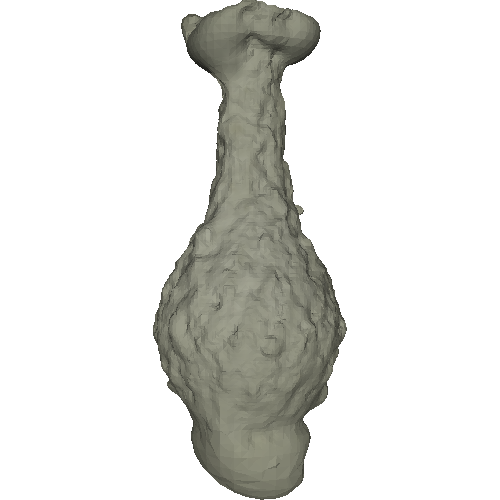
\includegraphics[width=0.1\textwidth]{interp/synth_interp/vase0_mvs}}&
\raisebox{-.5\height}{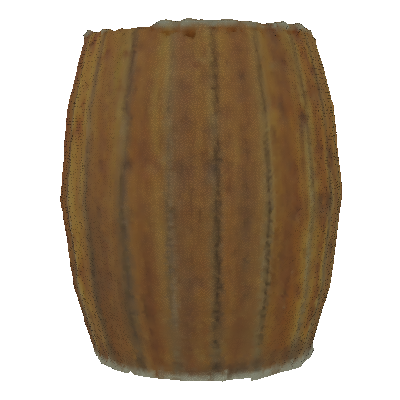
\includegraphics[width=0.1\textwidth]{interp/synth_interp/barrel_mvs}}&
\fcolorbox{green}{white}{\raisebox{-.5\height}{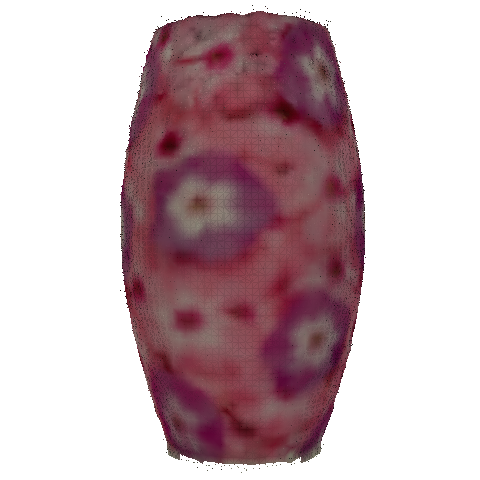
\includegraphics[width=0.1\textwidth]{interp/synth_interp/vase2_mvs}}}&
PMVS\\
\bottomrule
\end{tabular}
\caption{The evaluation of interpreter using synthetic objects. The first column presents the description provided to the interpreter. Description $i$ matches with condition $i$ in Table~\ref{tab:synth_prop_list}. The last column is the algorithm selected by the interpreter. The object of which condition matches the description is labeled in green rectangle. Since the interpreter would return a successful reconstruction given a description that matches the condition, the quality of reconstruction of the labeled objects indicates success/failure of the interpreter.}
\label{fig:synth_results}
\end{figure*}

\subsubsection{Data 1: Bust}

\subsubsection{Data 2: Vase1}

\subsubsection{Data 3: Barrel}
Description 1 matches with object \textit{barrel}, which has a reliable reconstruction result. The selected algorithm GSL is also in the mapped algorithms of object \textit{bust}, as shown in Table~\ref{tab:synth_prop_list}. Thus even though \textbf{description 1} doesn't match with the problem condition of \textit{bust}, a satisfactory result is also returned. However, the selected algorithm is not in the mapped algorithms of object \textit{vase0} and \textit{vase1}, thus less successful results are returned.

\subsubsection{Data 4: Vase2}

\subsection{Real-world Datasets}
We use similar setups to the synthetic counterparts and captured a real world dataset of nine objects~\ref{fig:test_real_world}. The property of these objects are listed in Table~\ref{tab:real_data_prop_list}. Since we do not have the ground truth here, we resort to visual analysis to see if the appropriate algorithm gives an acceptable reconstruction compared to that of the baseline method.
\begin{figure}[!htbp]
\centering
\begin{tabular}{c|*{4}{p{2cm}}}
\toprule
class \# & 1 & 2 & 3 & 4\\
\midrule
  & textureless & textureless & textured & textured\\
description & diffuse & mixed d/s & diffuse & mixed d/s\\
  & bright & bright & dark/bright & dark/bright\\
\hline
object & 
\raisebox{-.5\height}{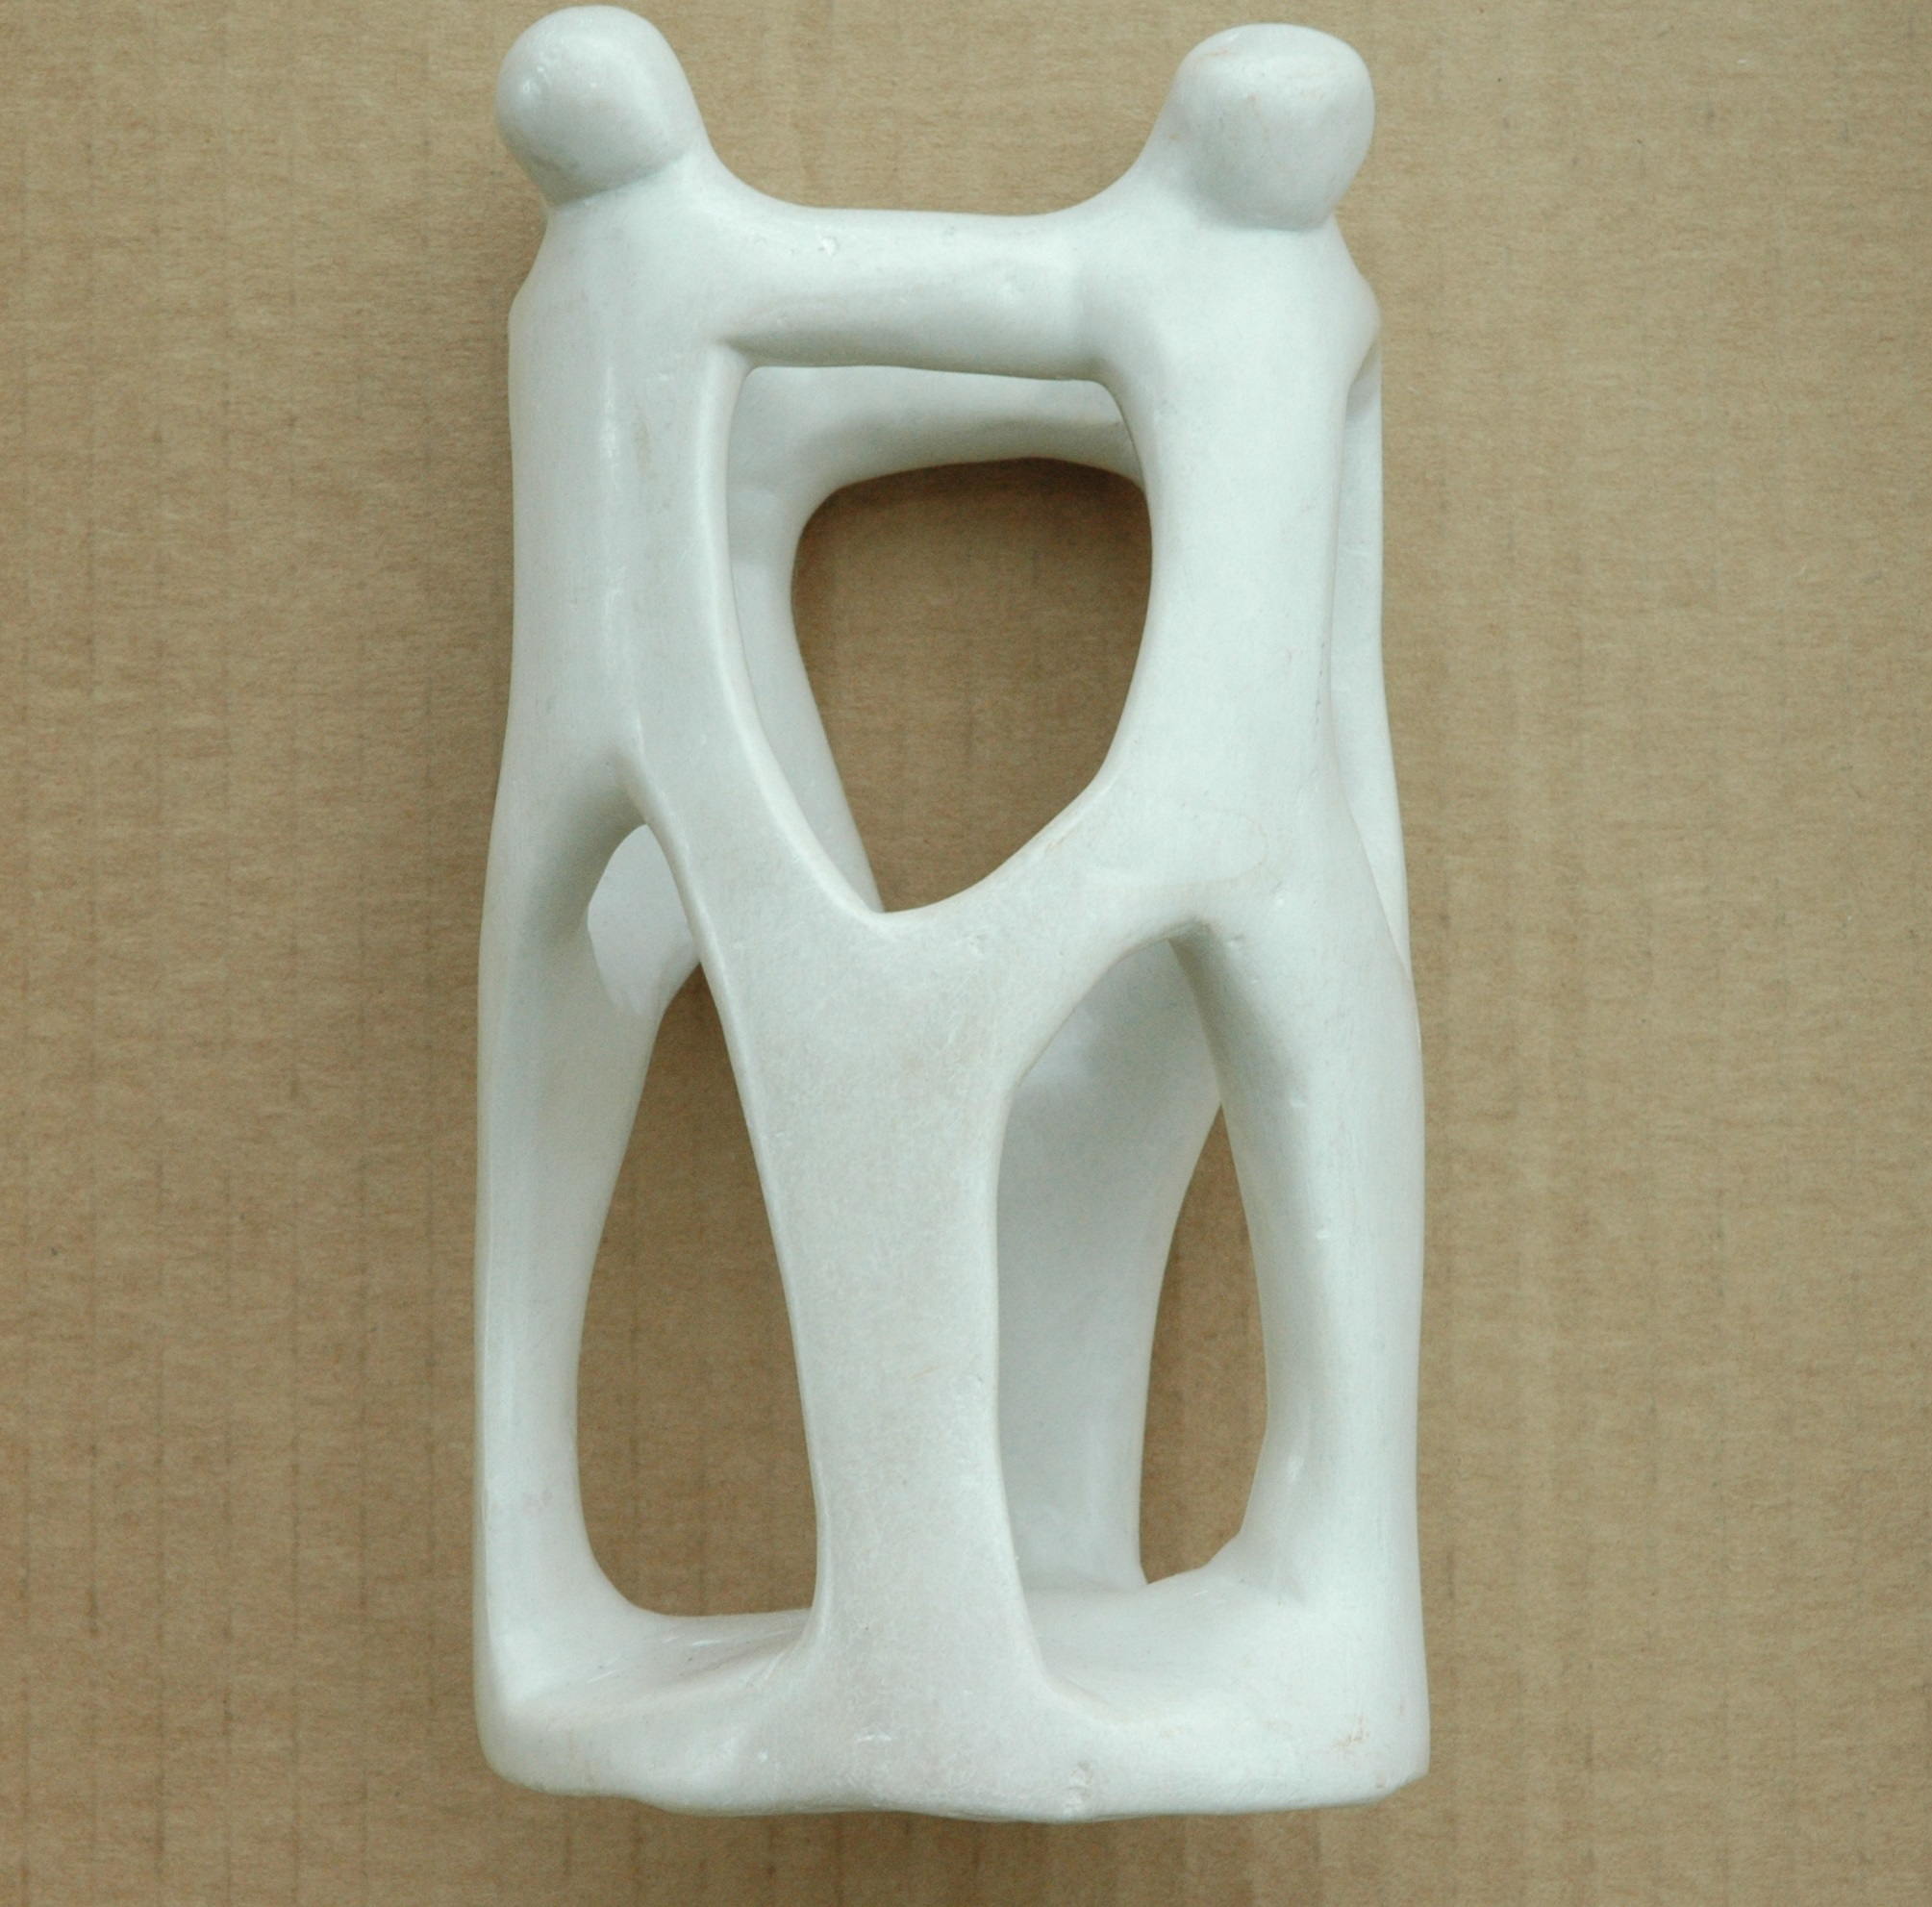
\includegraphics[width=0.15\textwidth]{interp/real_world_img/statue/statue}} &
\raisebox{-.5\height}{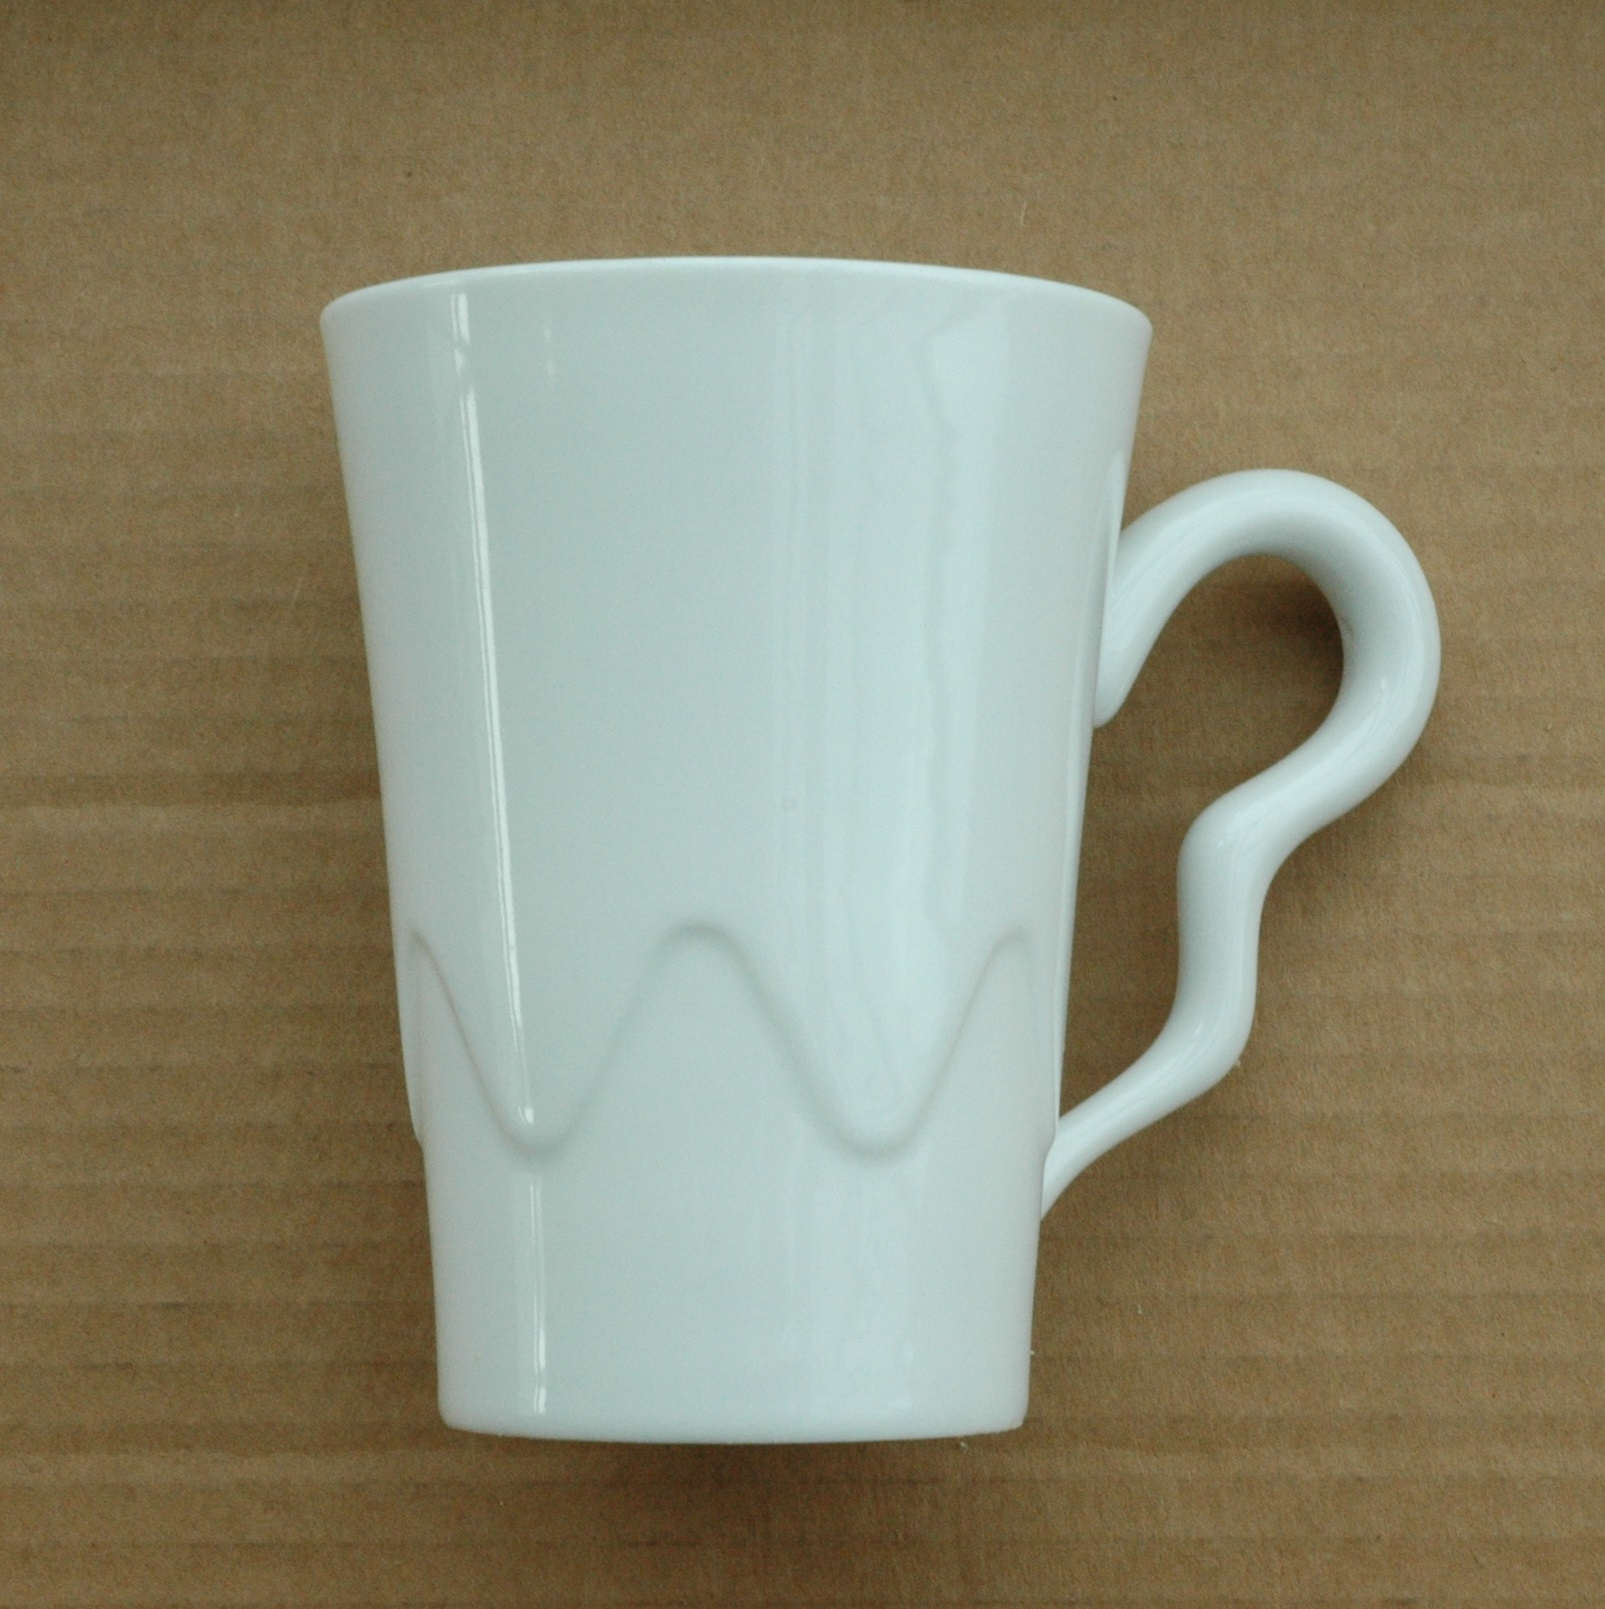
\includegraphics[width=0.15\textwidth]{interp/real_world_img/cup/cup}} &
\raisebox{-.5\height}{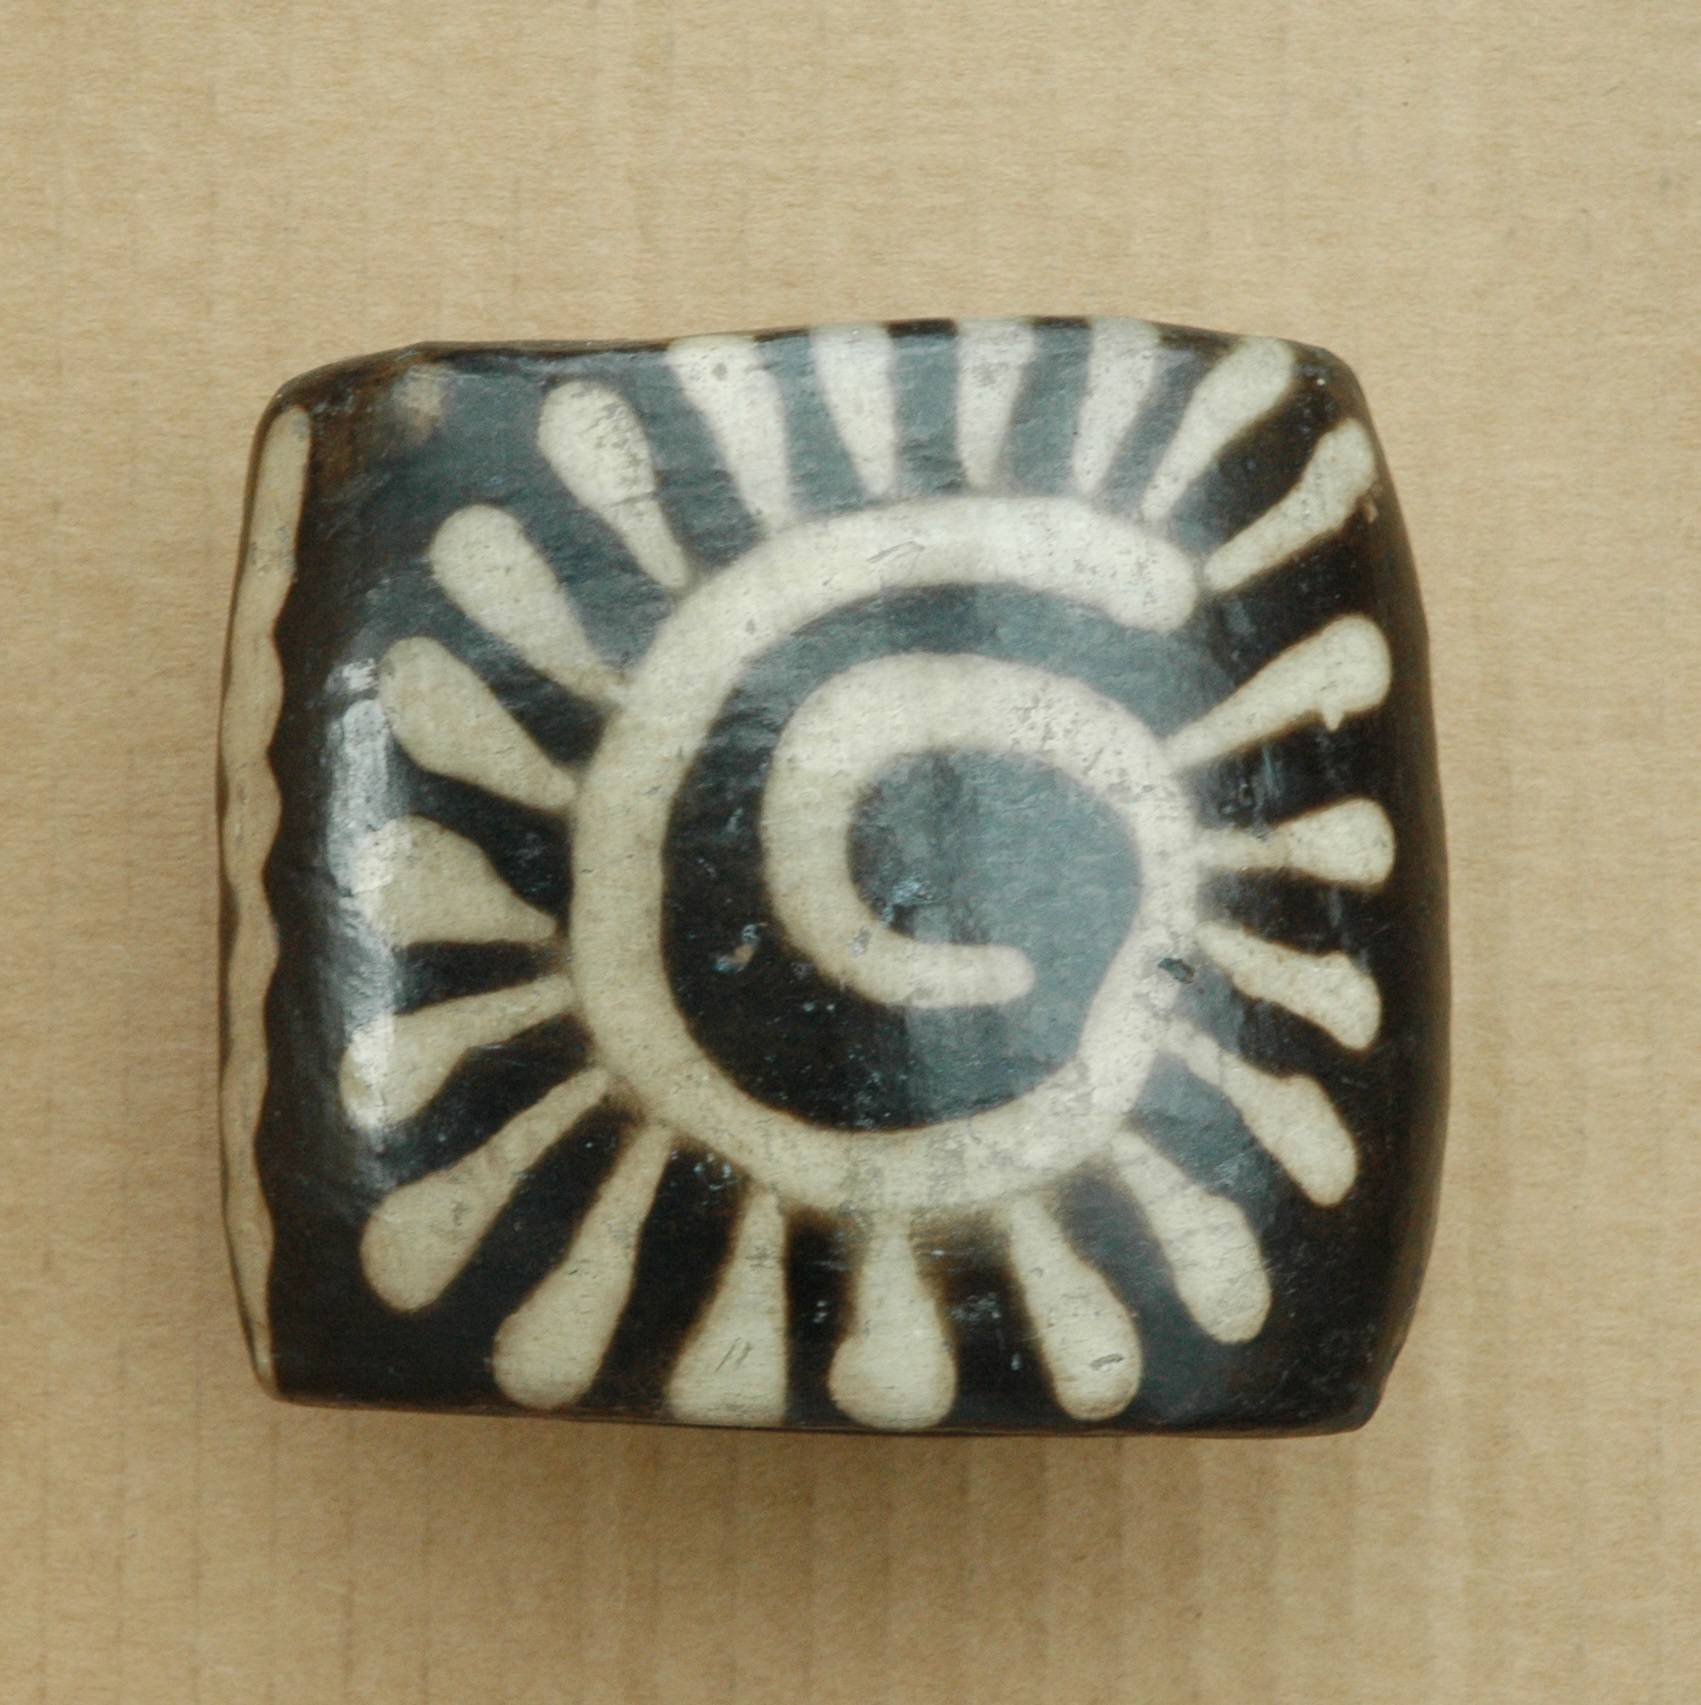
\includegraphics[width=0.15\textwidth]{interp/real_world_img/pot/pot}} &
\raisebox{-.5\height}{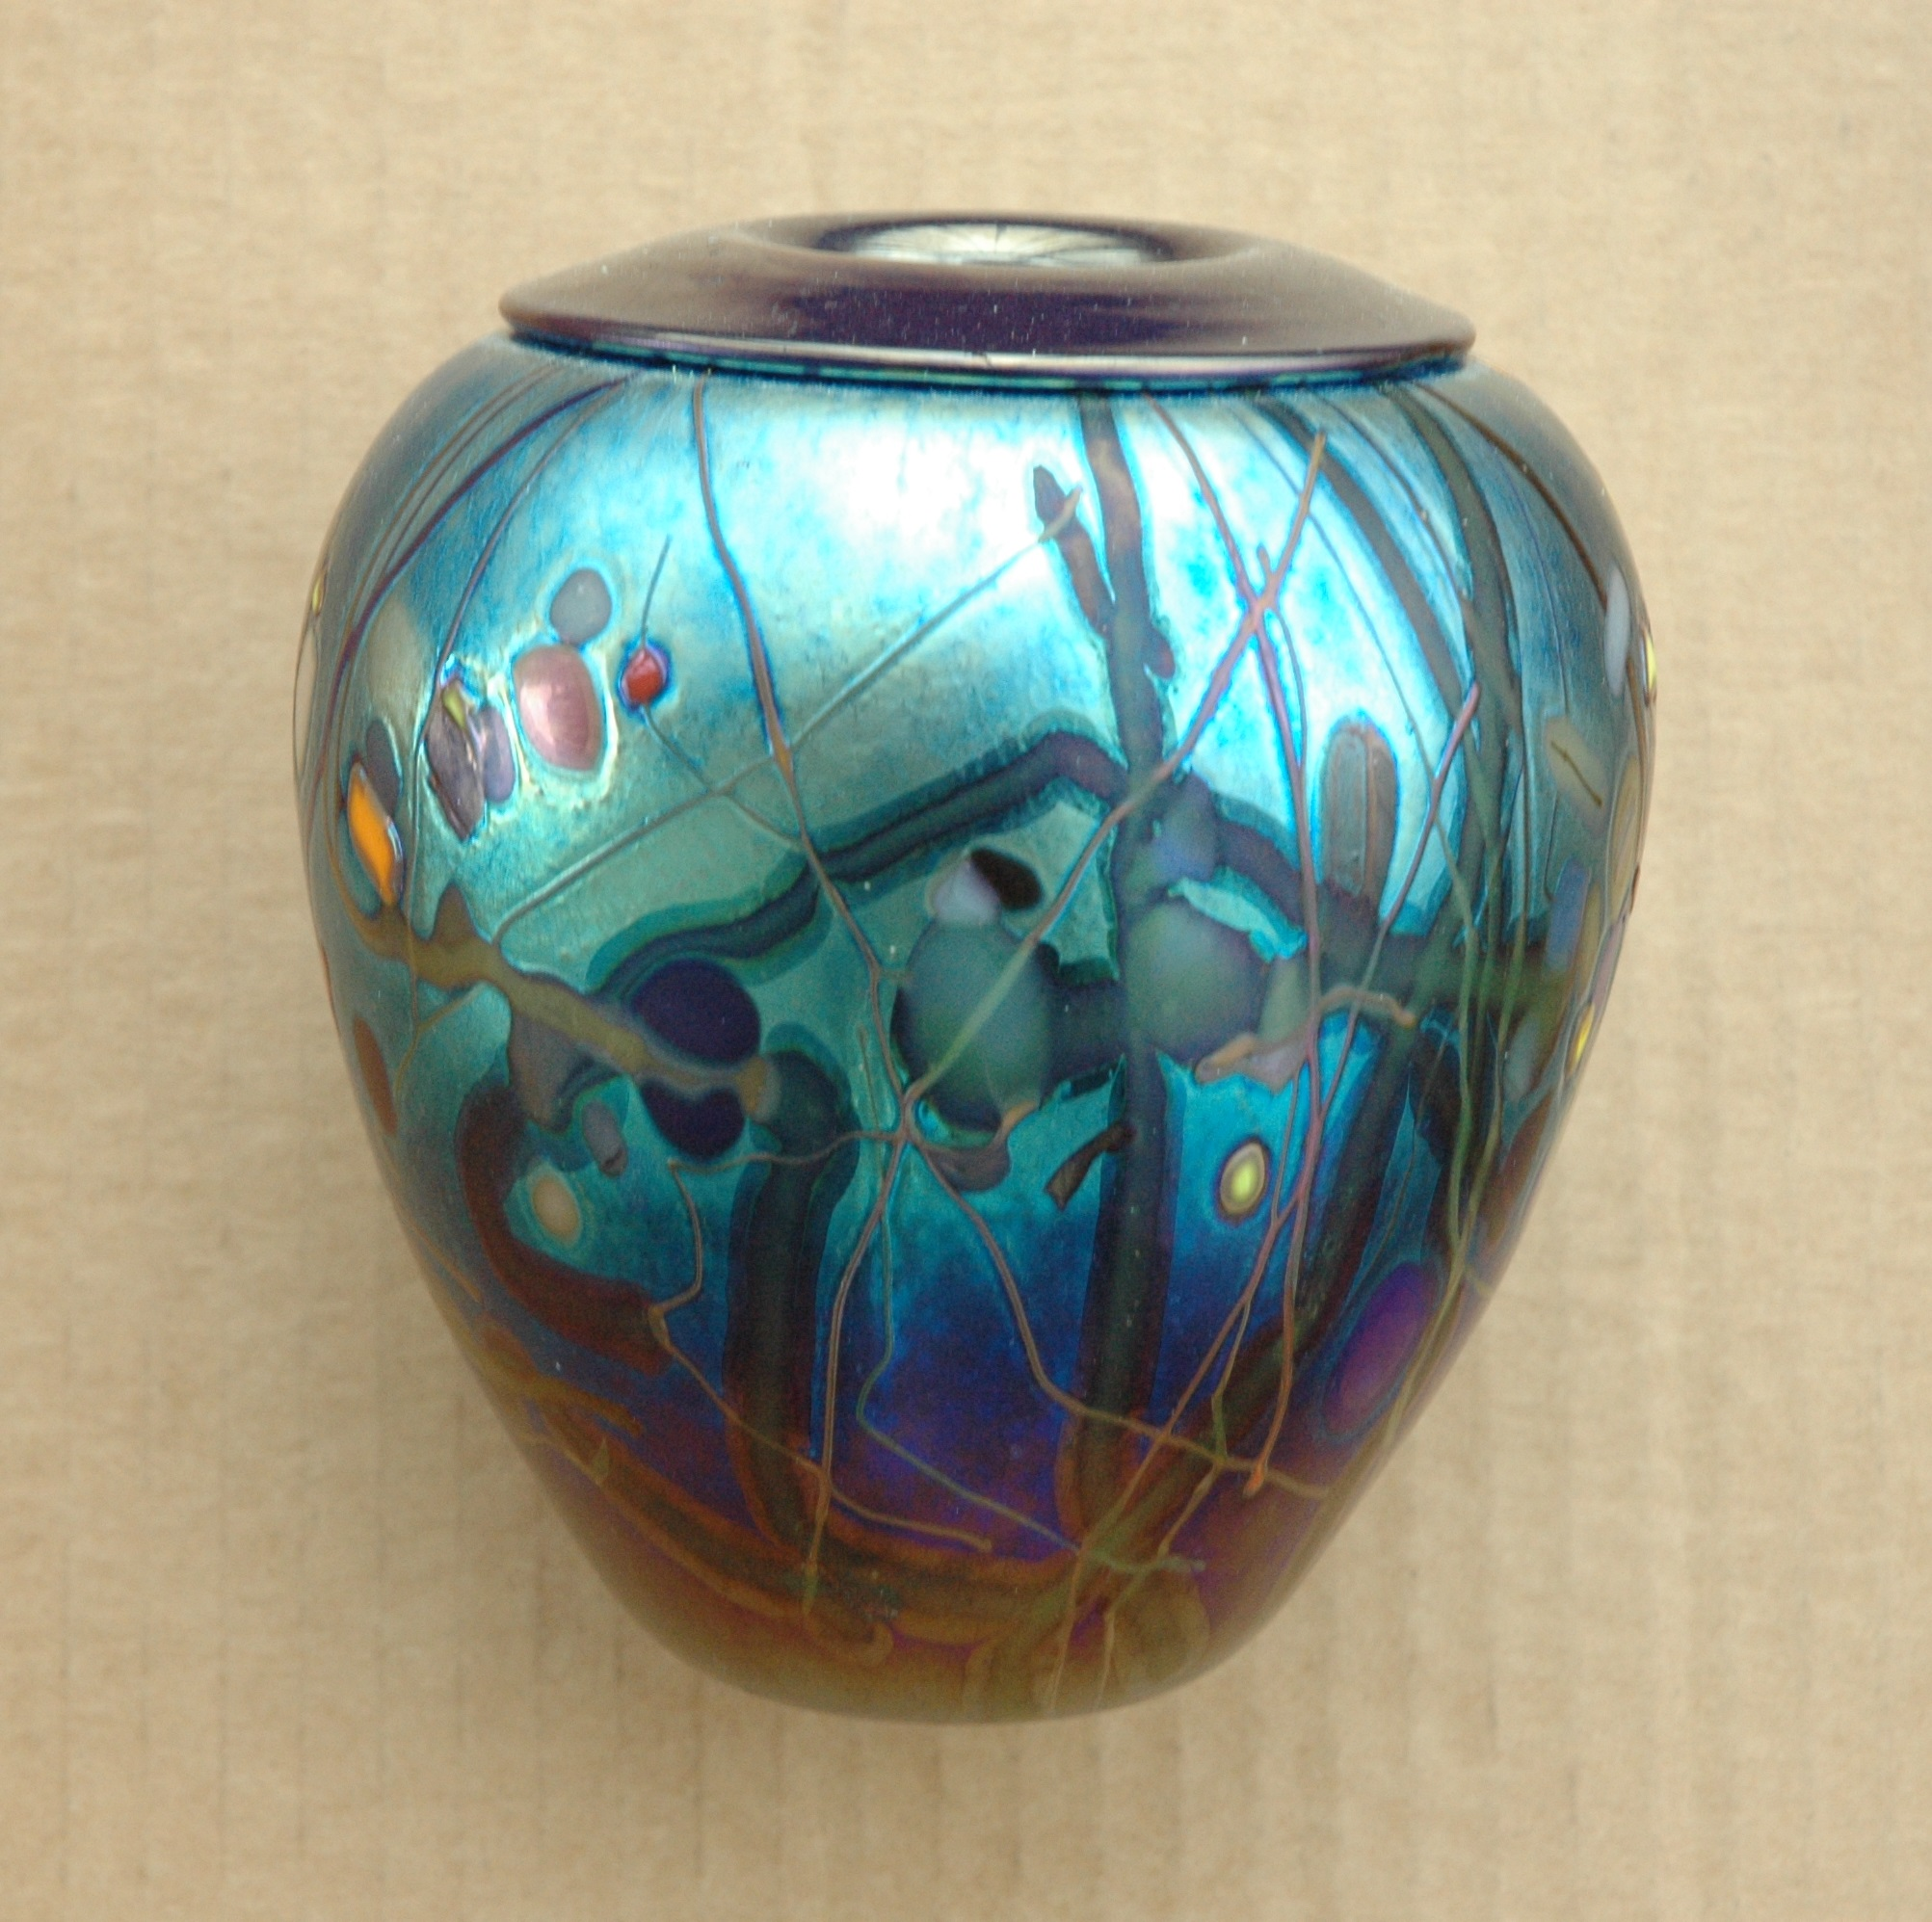
\includegraphics[width=0.15\textwidth]{interp/real_world_img/vase/vase}}\\
\bottomrule
\end{tabular}
\caption{The rerepsentatives of the four classes of objects used for evaluation.}
\label{fig:test_real_world}
\end{figure}

We use the aforementioned methods to retrieve the parameters of each property. The decomposition of material for each object is presented in Figure~\ref{fig:real_data_material}. The property settings of each object is listed in Table~\ref{tab:real_data_prop_list}.
\begin{table}[!htbp]
  \centering
  \begin{tabular}{lllllll}
  \toprule
  C\# & Object & Texture & Albedo & Specular & Rough & Mapping\\
  \midrule
  1 & statue & 0.2 & 0.8 & 0.2 & 0.8 & EPS, GSL\\
  2 & cup & 0.2 & 0.8 & 0.5 & 0.2 & EPS, GSL\\
  3 & pot & 0.8 & 0.8 (0.2) & 0.2 & 0.2 & PMVS, GSL\\
  4 & vase & 0.8 & 0.8 (0.2) & 0.5 & 0.2 & PMVS\\
  \bottomrule
  \end{tabular}
  \caption{Problem conditions and mapping for the real-world objects}
  \label{tab:real_data_prop_list}
\end{table}

% \begin{table}[!htbp]
%   \centering
%   \begin{tabular}{l*{5}{c}}
%   \hline
%   \textbf{Object} & Texture & Albedo & Specular & Rough & Mapping\\
%   \hline
%   status & 0.2 & 0.8 & 0.2 & 0.8 & EPS, GSL\\
%   cup & 0.2 & 0.8 & 0.5 & 0.2 & EPS, GSL\\
%   pot & 0.8 & 0.2, 0.5 & 0.2 & 0.2 & PMVS\\
%   vase & 0.8 & 0.2, 0.5 & 0.5 & 0.2 & PMVS\\
%   \hline
%   \end{tabular}
%   \caption{Property list for the real-world objects}
%   \label{tab:real_data_prop_list}
% \end{table}

% \begin{table}[!hbtp]
%   \centering
%   \begin{tabular}{*{12}{c}}
%   \multicolumn{3}{l}{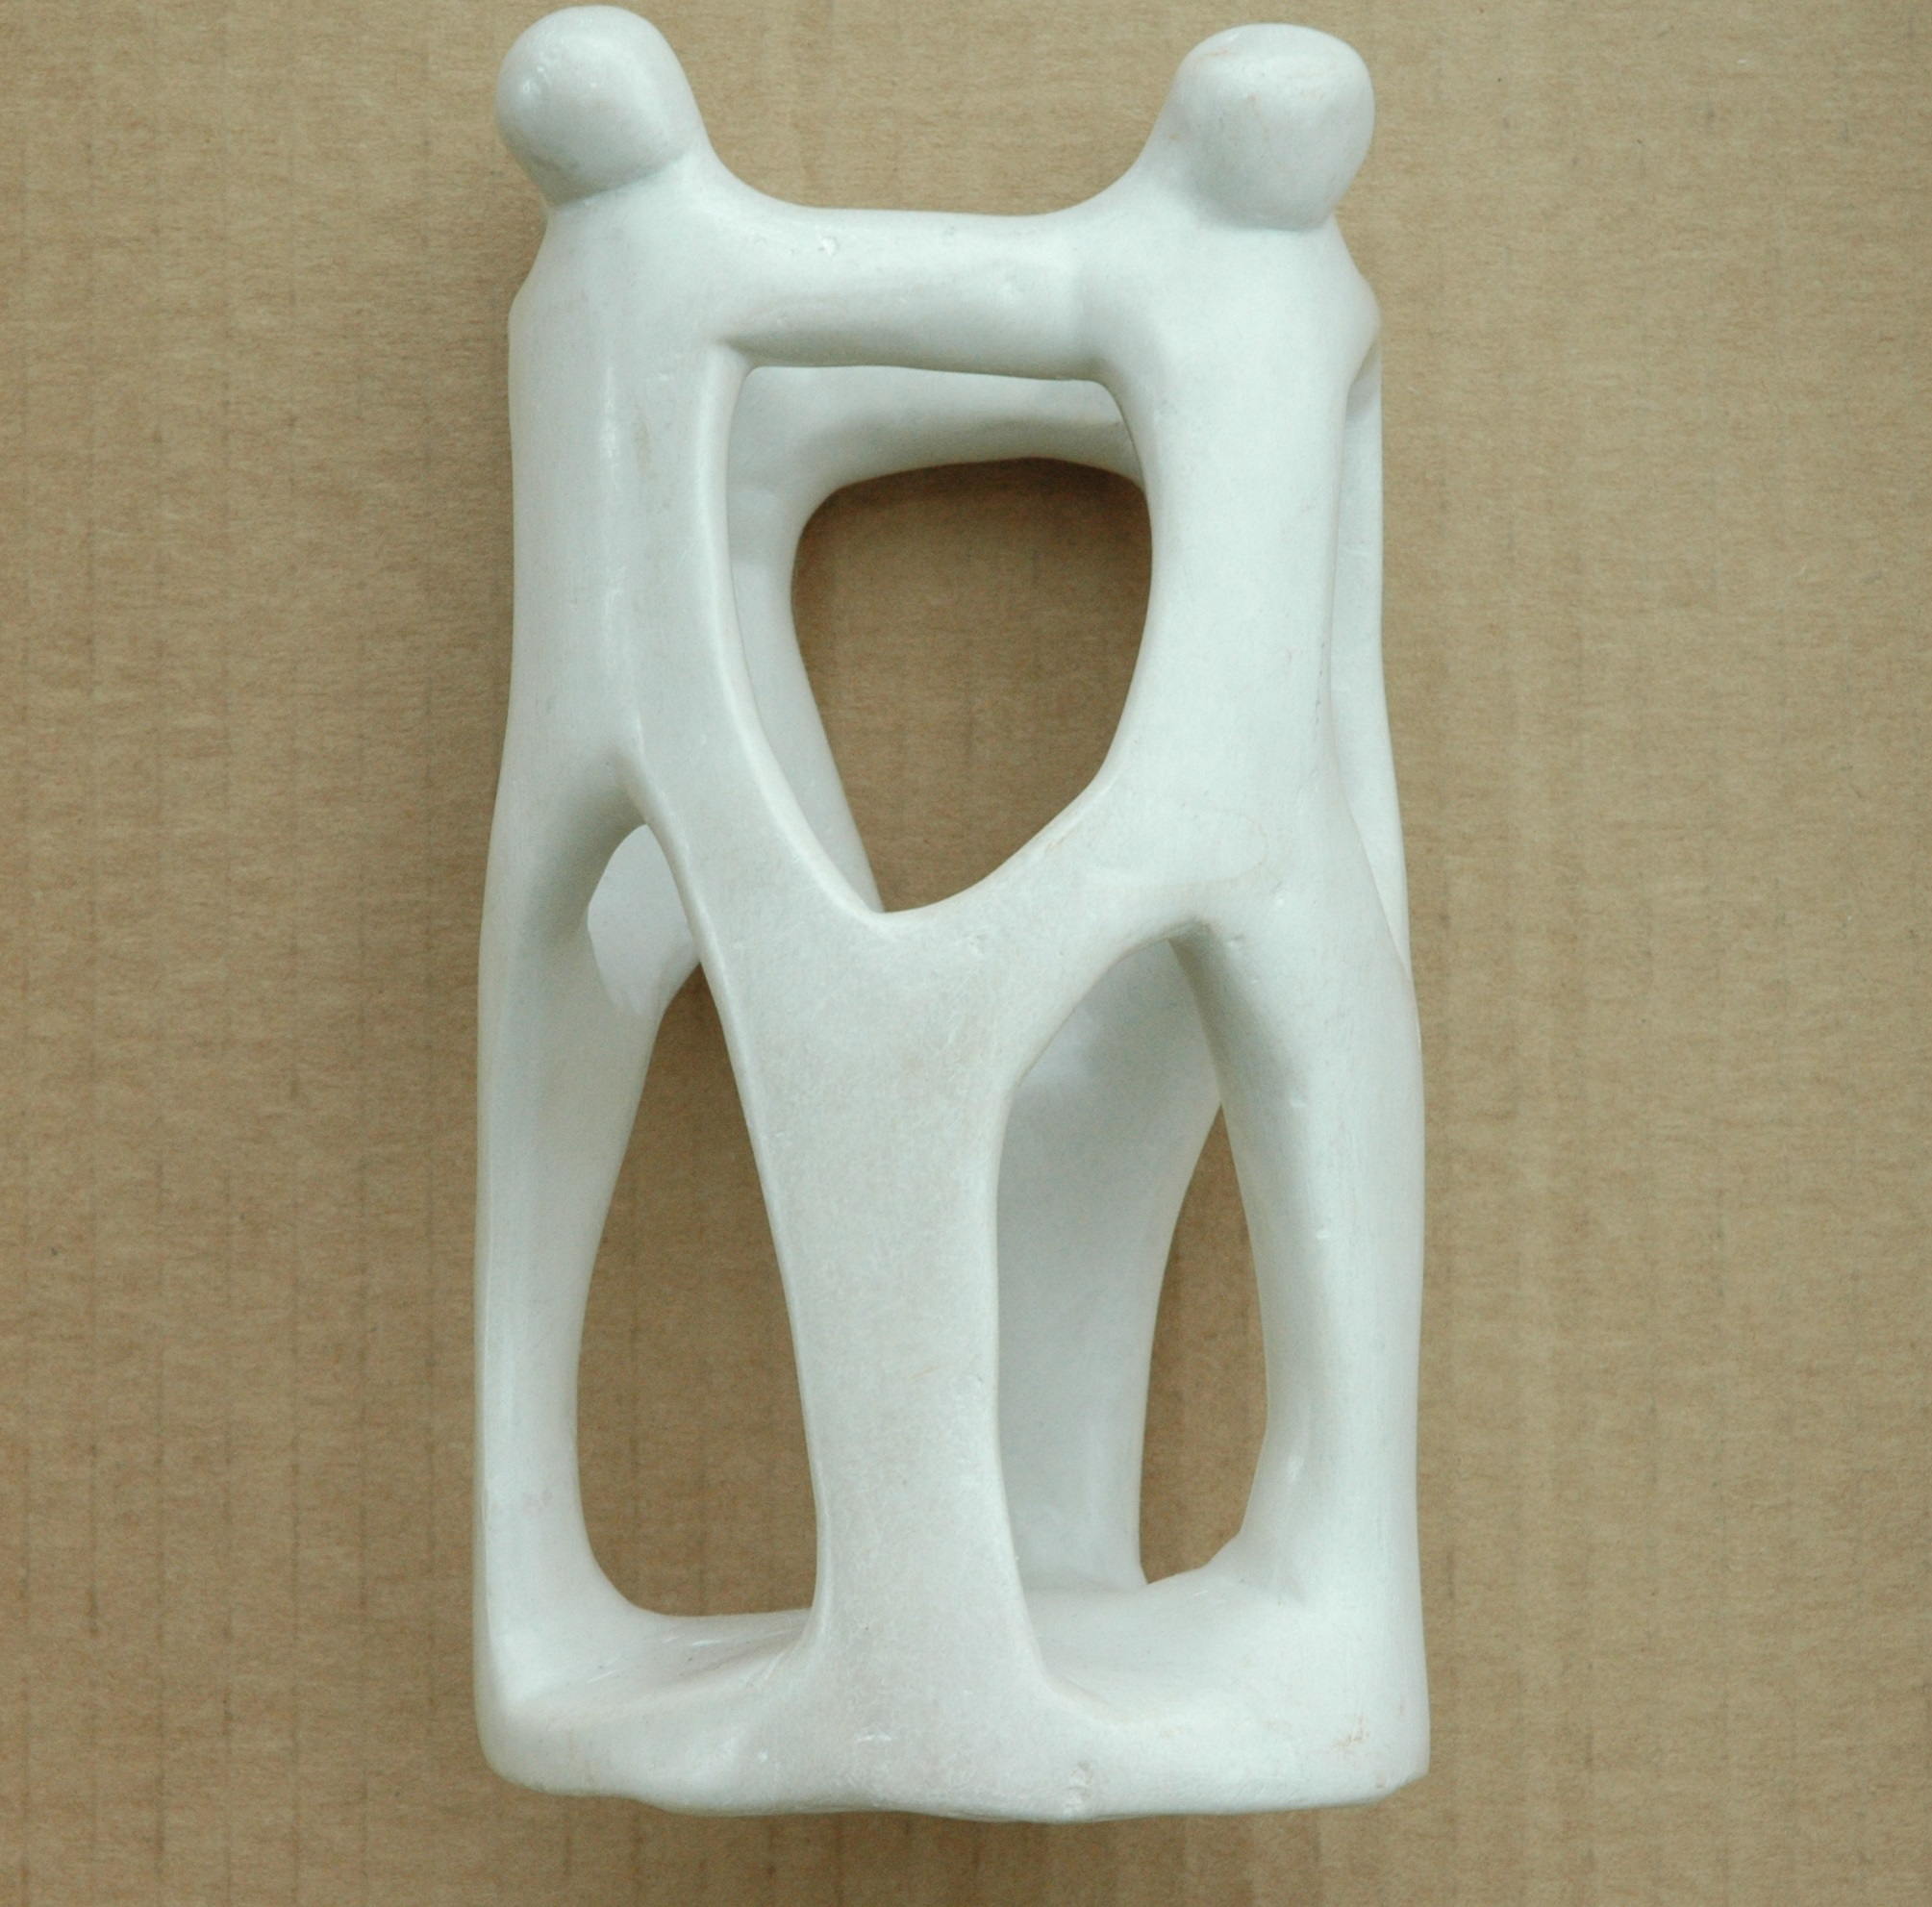
\includegraphics[width=0.25\textwidth]{interp/real_world_img/statue/statue}} &
%   \multicolumn{3}{l}{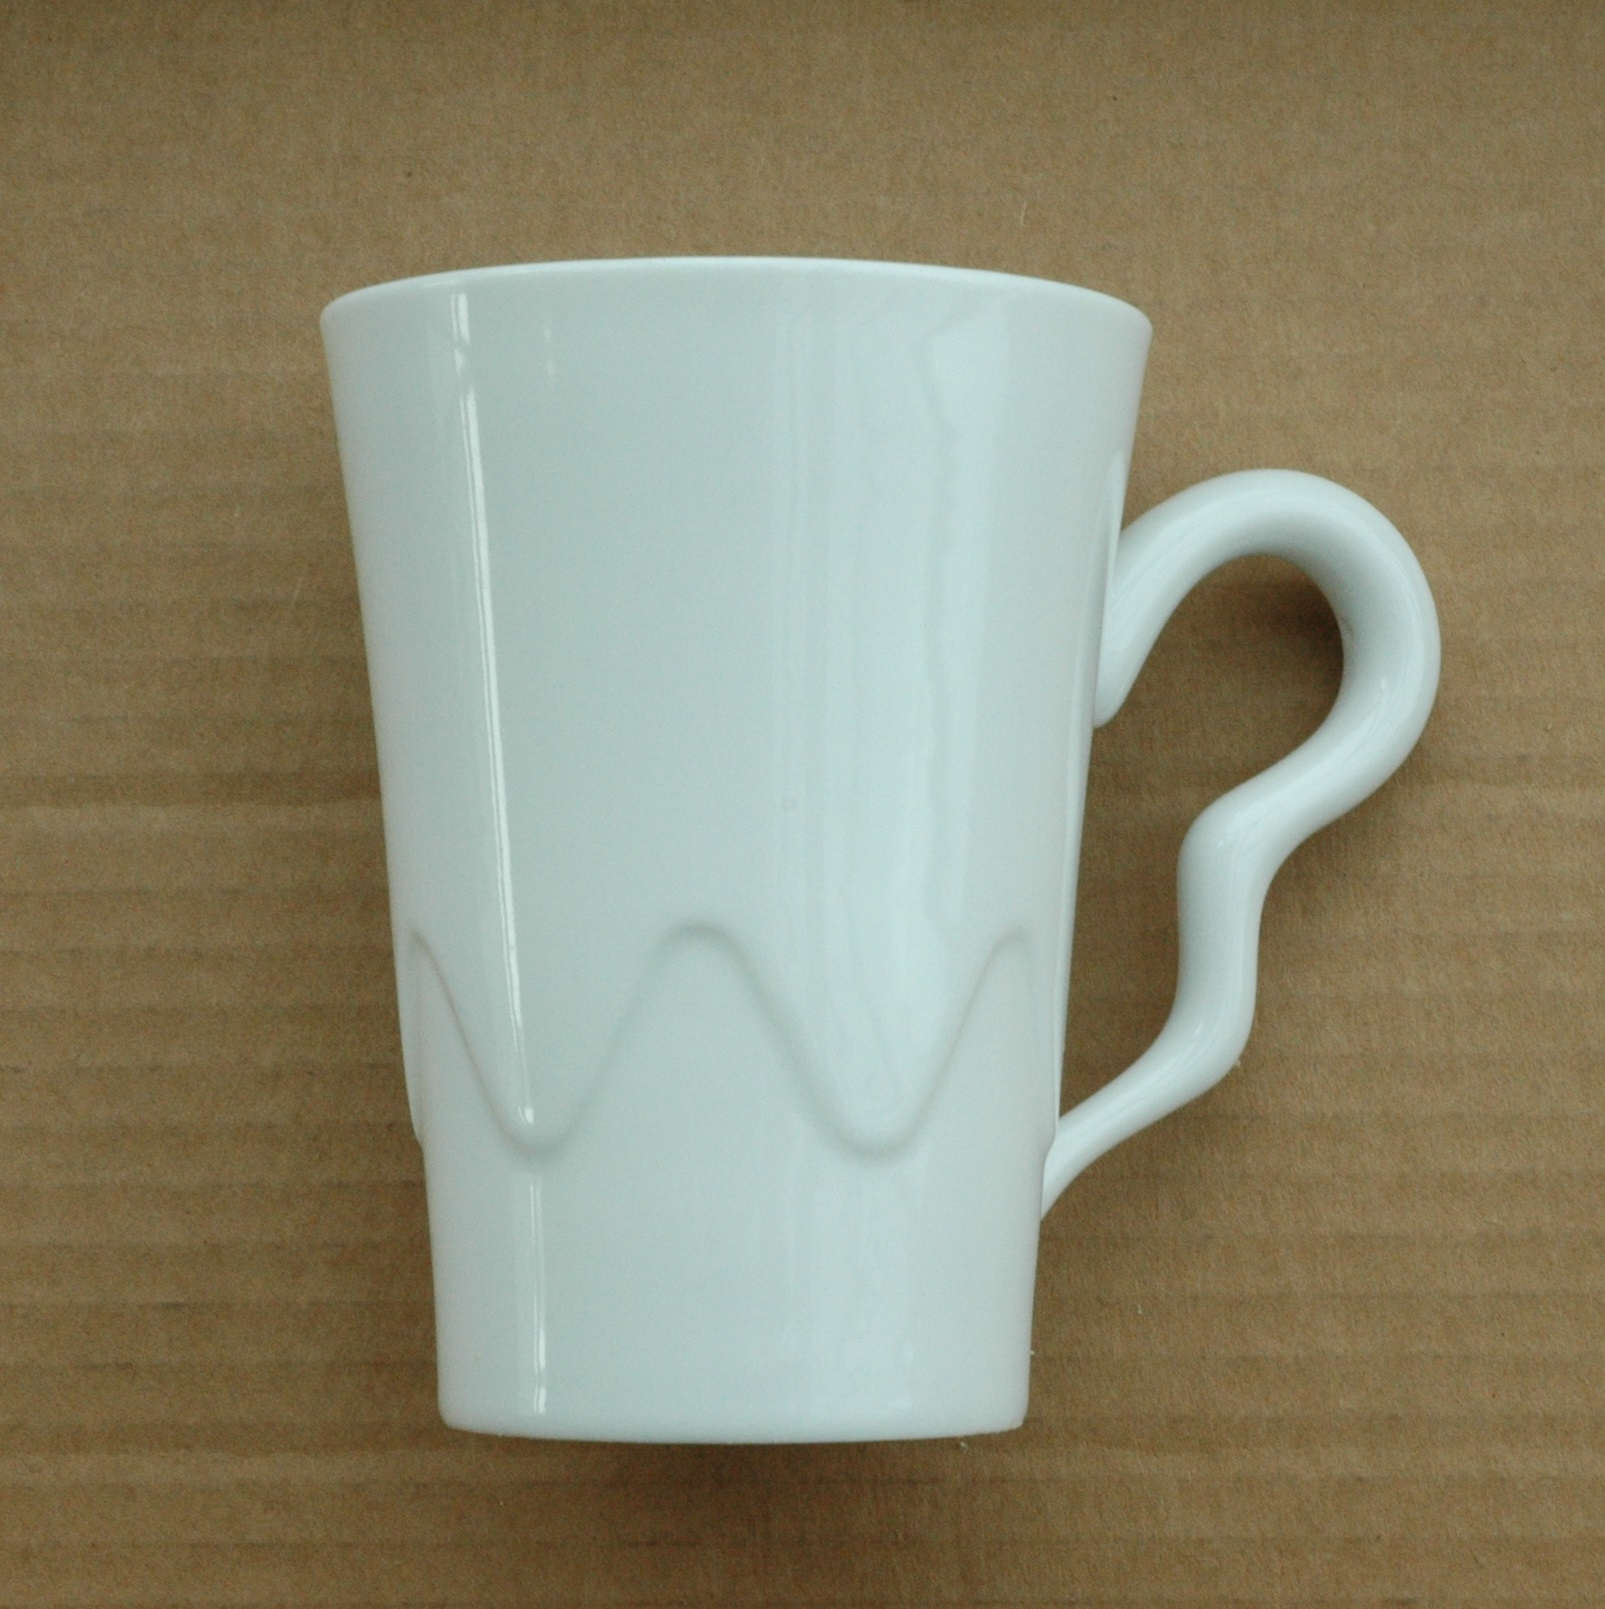
\includegraphics[width=0.25\textwidth]{interp/real_world_img/cup/cup}} &
%   \multicolumn{3}{l}{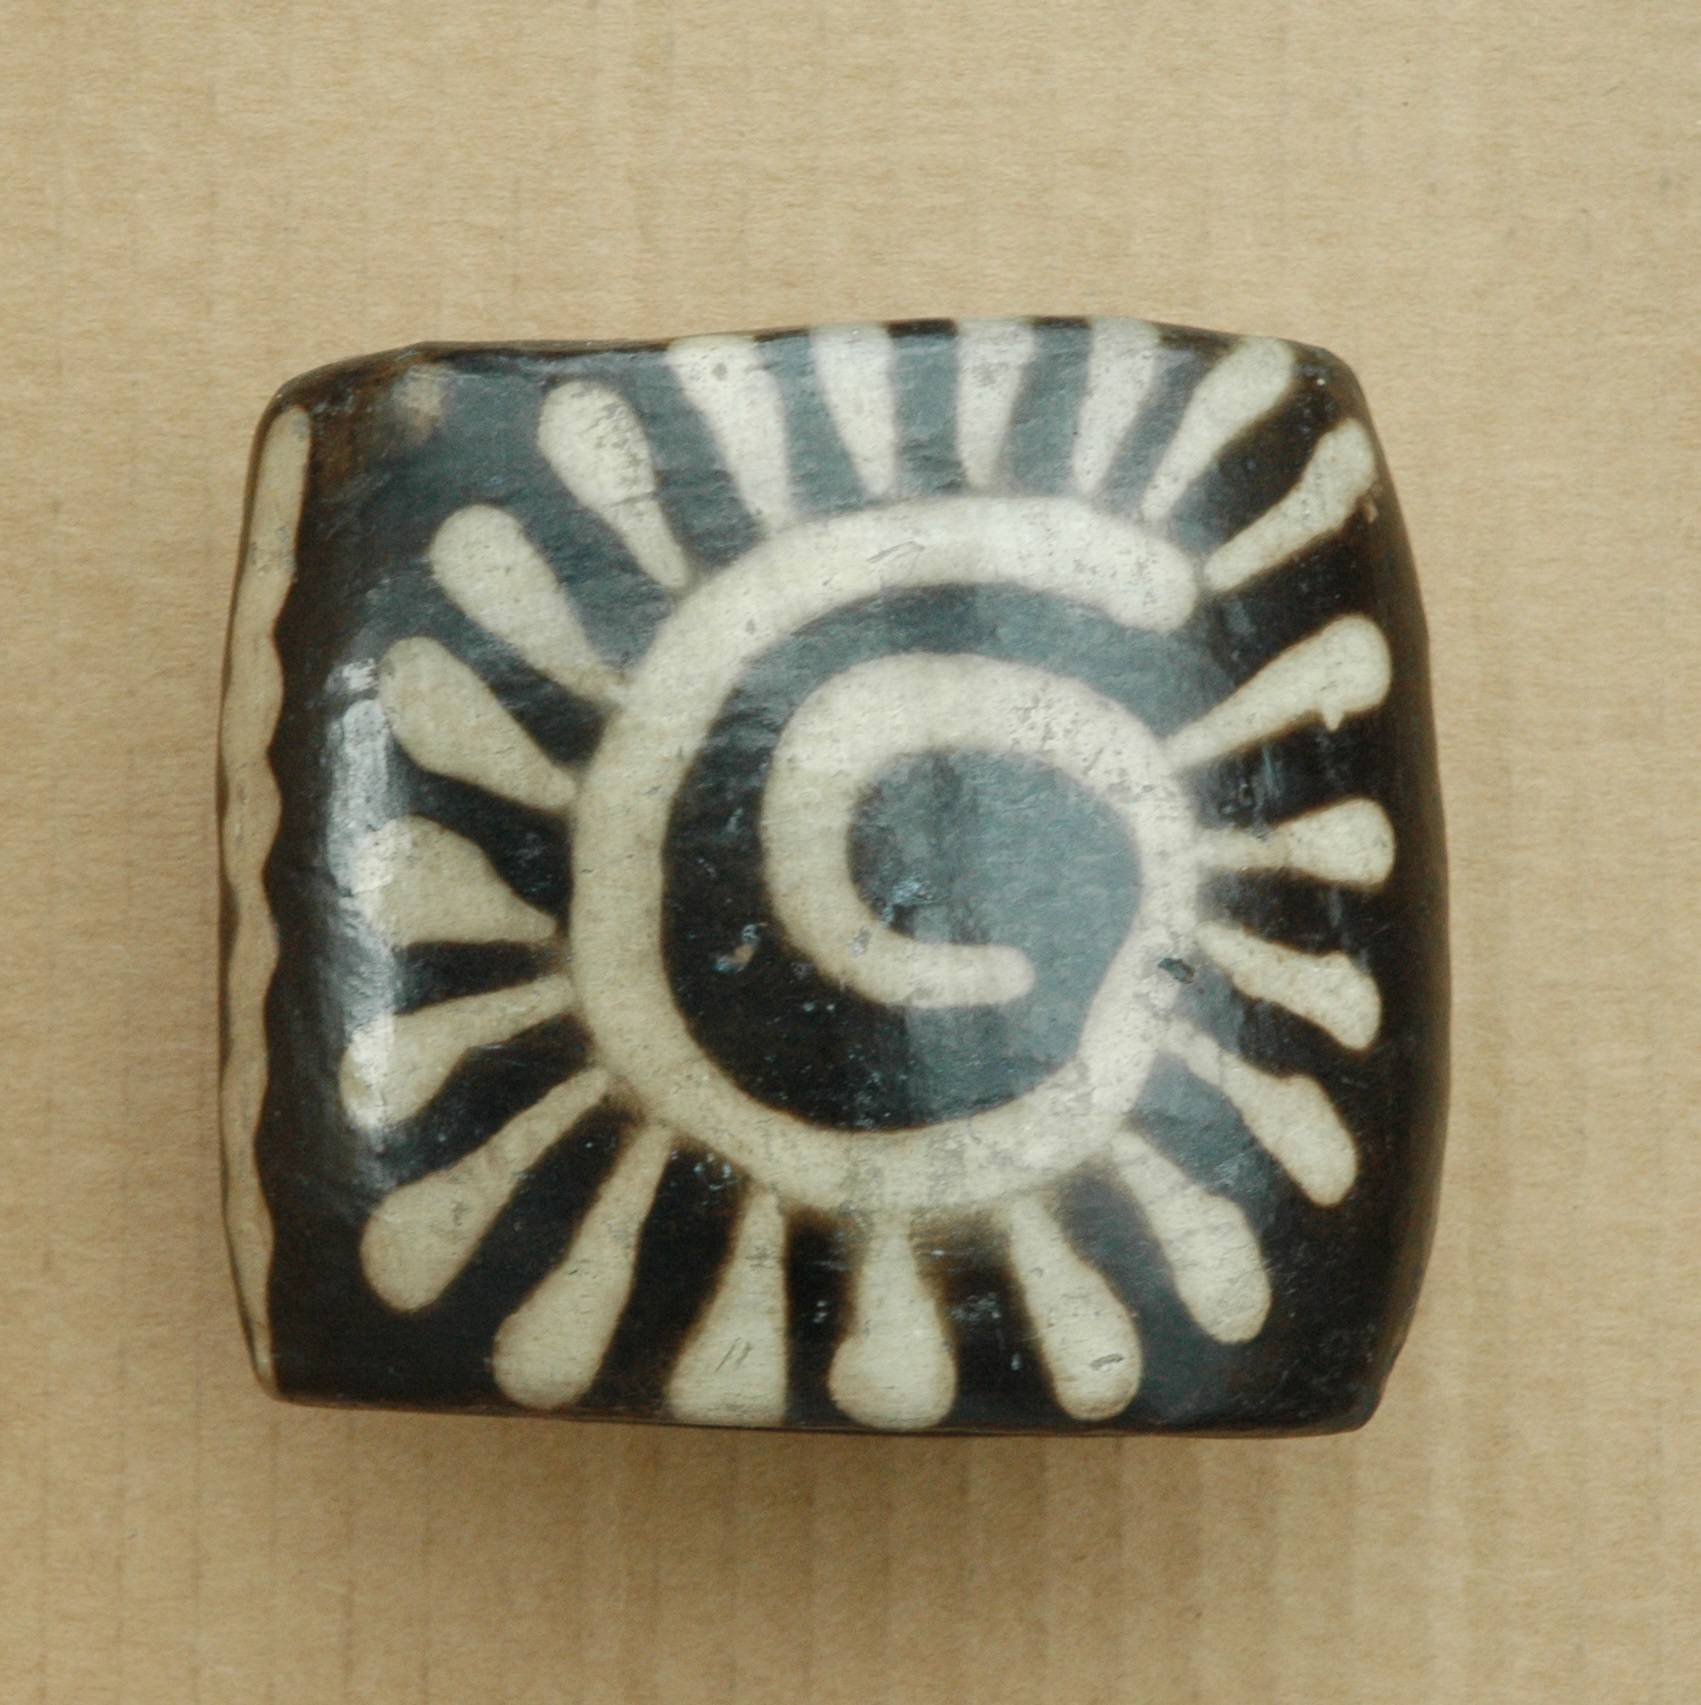
\includegraphics[width=0.25\textwidth]{interp/real_world_img/pot/pot}} &
%   \multicolumn{3}{l}{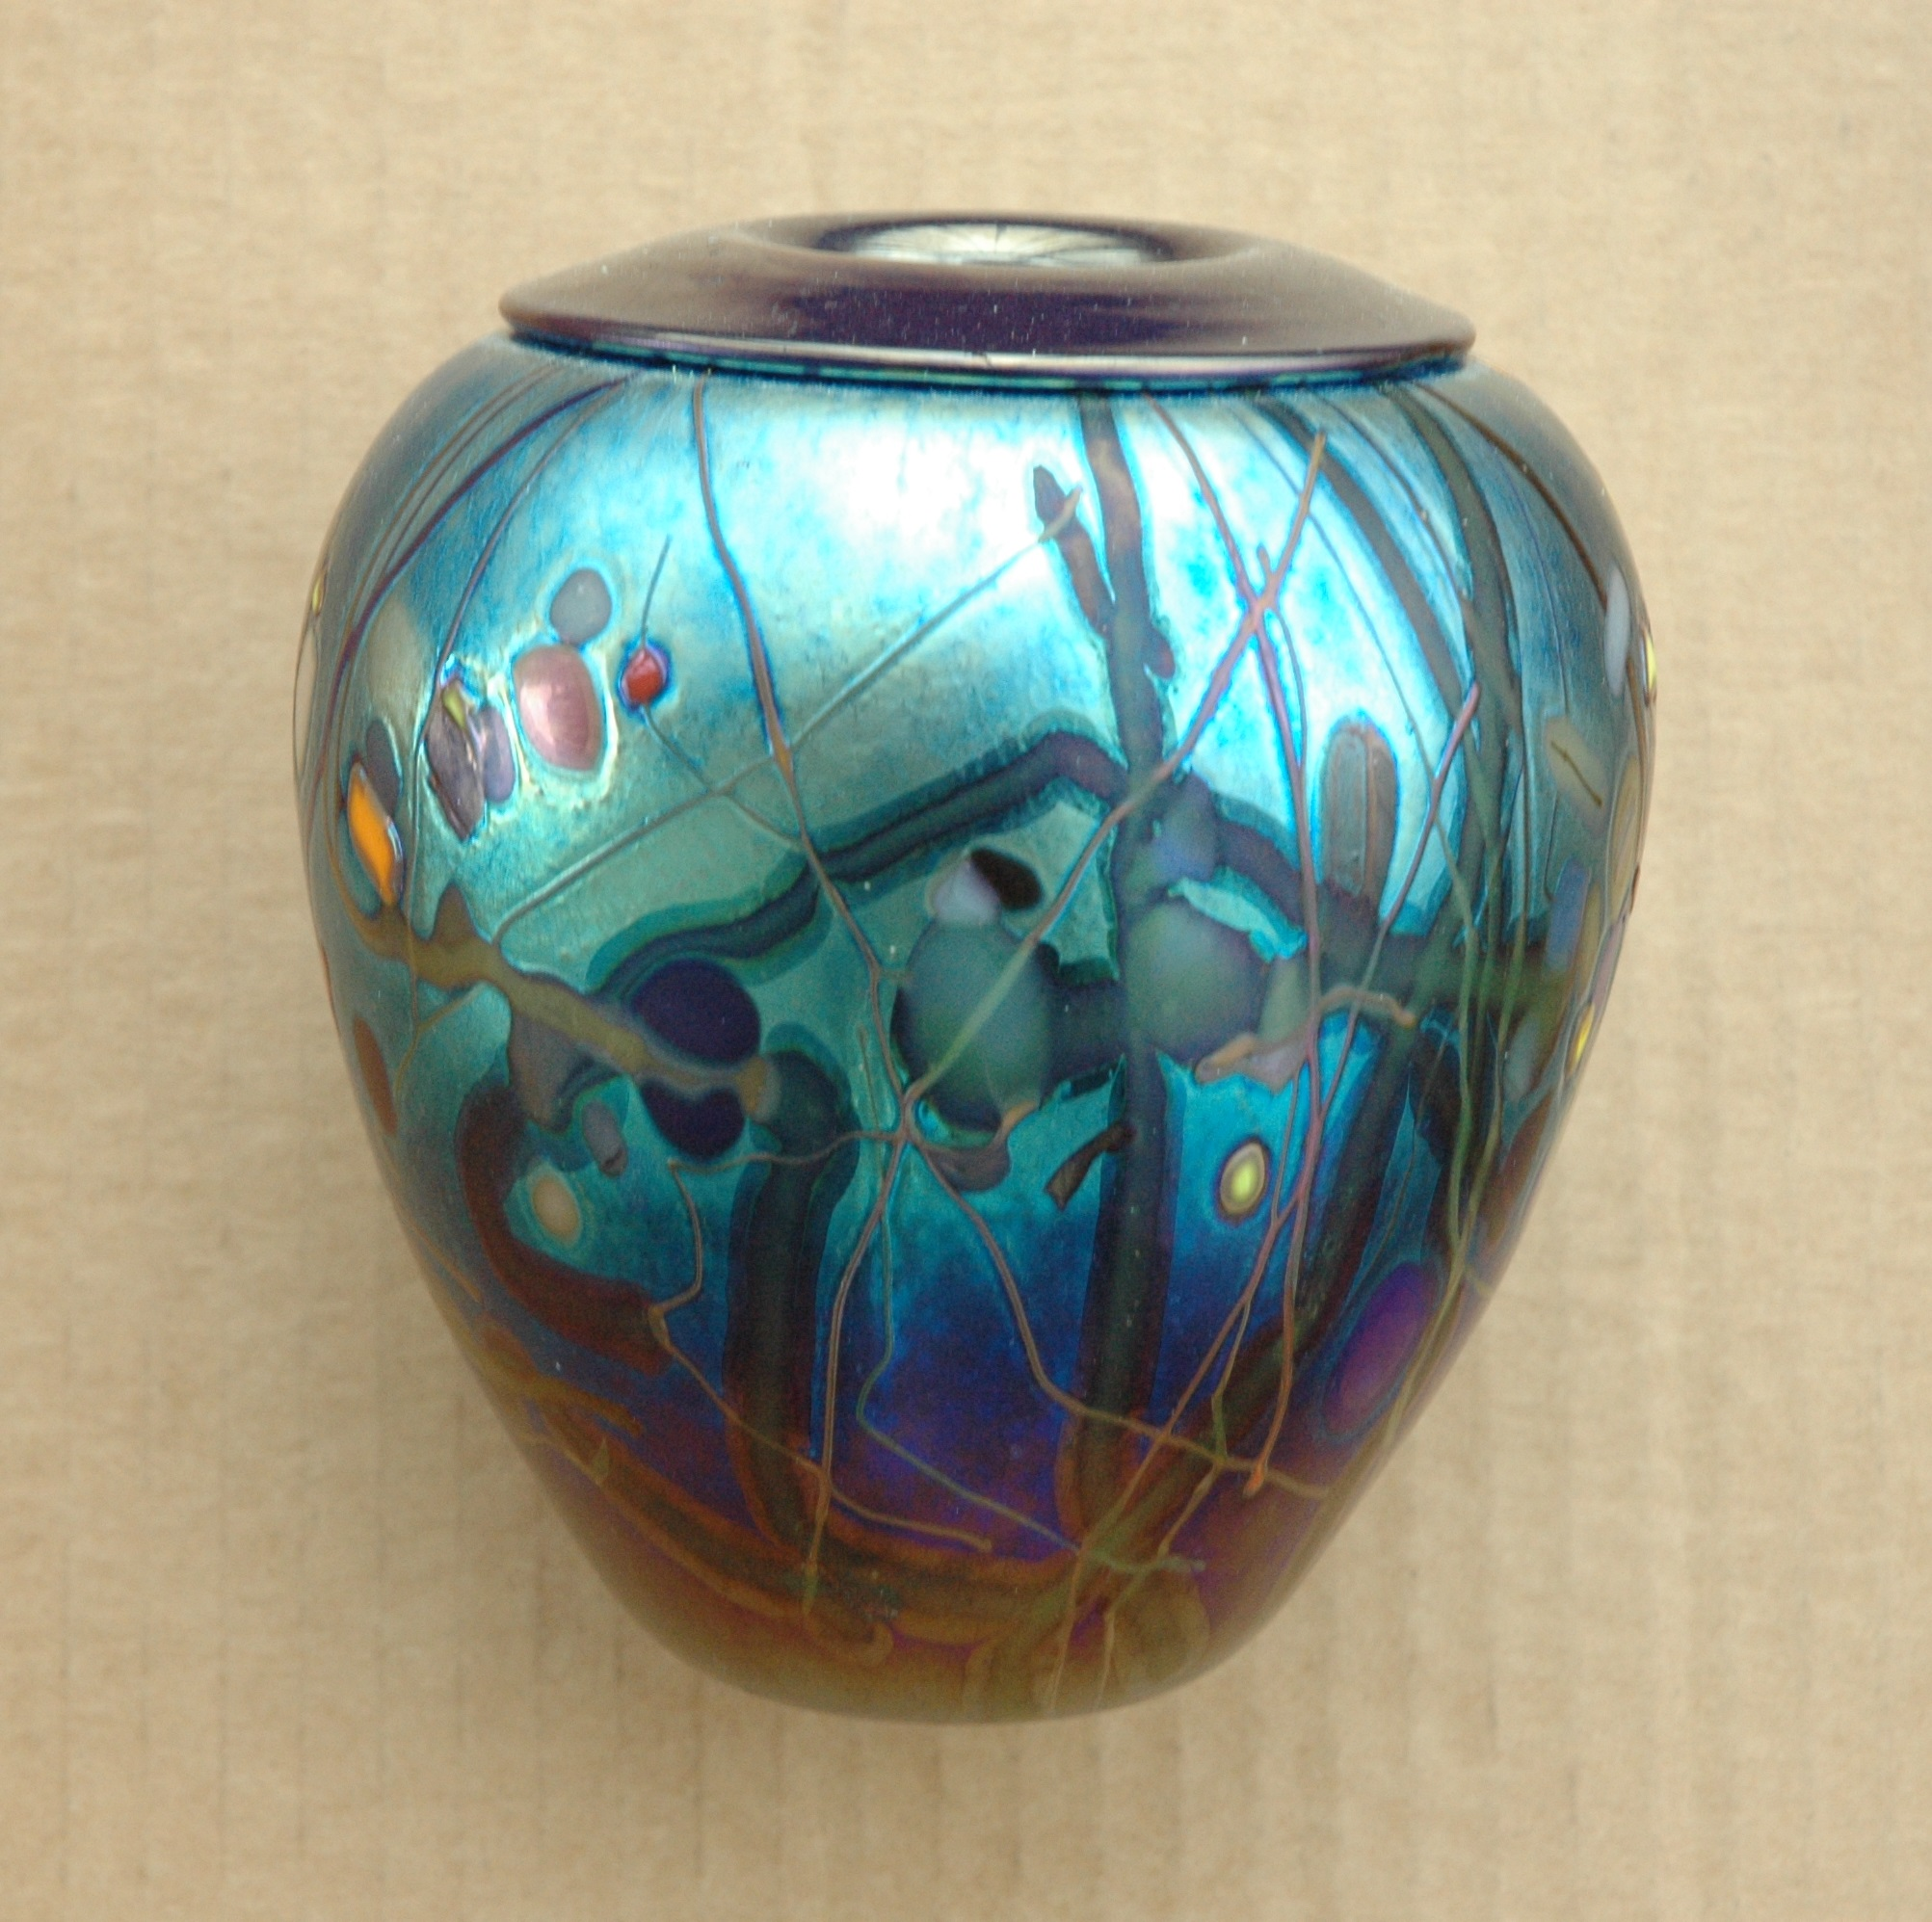
\includegraphics[width=0.25\textwidth]{interp/real_world_img/vase/vase}}\\
%   \includegraphics[width=0.1\textwidth]{interp/real_world_img/statue/base_00} & & &
%   \includegraphics[width=0.1\textwidth]{interp/real_world_img/cup/base_00} & &
%   \includegraphics[width=0.1\textwidth]{interp/real_world_img/pot/base_00} &
%   \includegraphics[width=0.1\textwidth]{interp/real_world_img/pot/base_01} & &
%   \includegraphics[width=0.1\textwidth]{interp/real_world_img/vase/base_00} &
%   \includegraphics[width=0.1\textwidth]{interp/real_world_img/vase/base_01}\\
%   \multicolumn{3}{c}{(d). statue} & \multicolumn{3}{c}{(e). cup} & 
%   \multicolumn{3}{c}{(g). pot} & \multicolumn{3}{c}{(i). vase} \\
%   \end{tabular}
%   \caption{Material of Real-world objects.}
%   \label{fig:real_data_material}
% \end{table}

\subsubsection{Data 1: statue}

\subsubsection{Data 2: cup}

\subsubsection{Data 3: pot}
Description 1 matches partially with object \textit{pot} since it has both high and low albedo surface areas. The surface area with high albedo is well reconstructed whereas the surface with low albedo, which doesn't match the description is not reconstructed at all. The selected algorithm is also in the mapped algorithms of object \textit{statue} and \textit{cup}, thus satisfactory results are returned as well. However, this is not the case for object \textit{vase}, thus a very sparse reconstruction is returned.

\subsubsection{Data 4: vase}

% \subsubsection{Data 1: statue}
% The first real-world object is a statue with low texture, low specular component, medium roughness, and high albedo. PMVS produces a very noisy reconstruction due to the lack of surface texture, whereas the other two techniques (EPS and GSL) return satisfactory results. The interpreter would thus return the appropriate result based on user specified constraints.

% \subsubsection{Data 2: cup}
% The second real-world object is a cup with low texture, low roughness, high albedo and high specular. PMVS fails to reconstruct the surface while EPS and GSL provide good results. The quality of detail of EPS are clearly higher than that of GSL, and the interpreter would return the result meets the constraints specified by the user.

% \subsubsection{Data 3: pot}
% The third object is a pot with high texture, low specular, medium roughness, and both high and low albedo values. PMVS gives a good reconstruction results, while EPS and GSL suffer due to low albedo.

% \subsubsection{Data 4: vase}
% The fourth object is a vase with high texture, high specular, low roughness, and both low and high albedo. PMVS shows good result, while EPS and GSL fail to reconstruct the surface due to low albedo and high specular.

\begin{figure*}[!htbp]
\centering
\begin{tabular}{lccccr}
\toprule
Desc \# & Statue & Cup & Pot & Vase & Selected Algo.\\
\midrule
1 &
\fcolorbox{green}{white}{\raisebox{-.5\height}{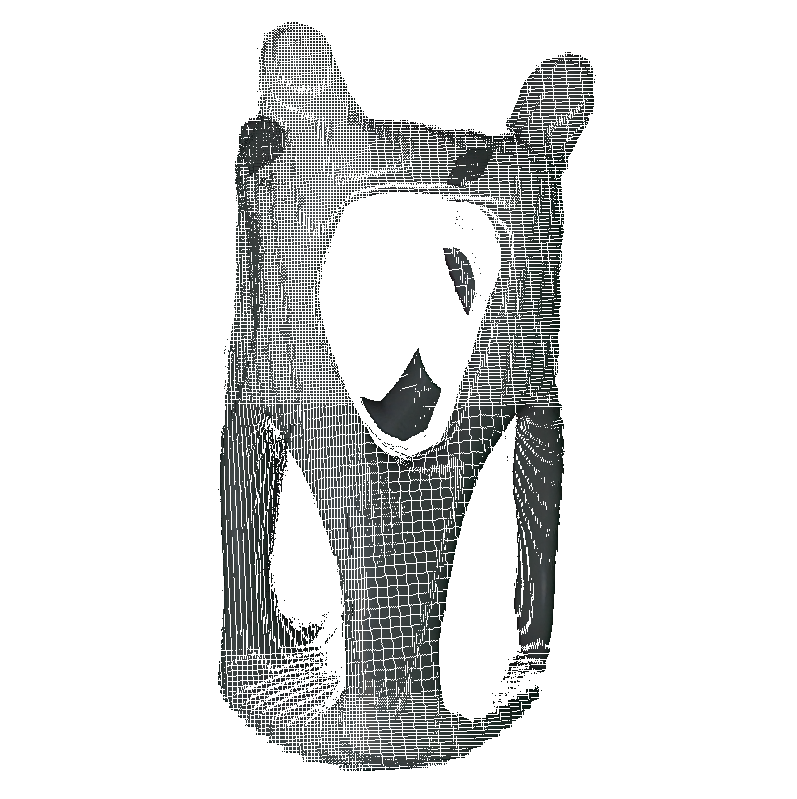
\includegraphics[width=0.1\textwidth]{interp/real_interp/statue/statue_sl}}}&
\raisebox{-.5\height}{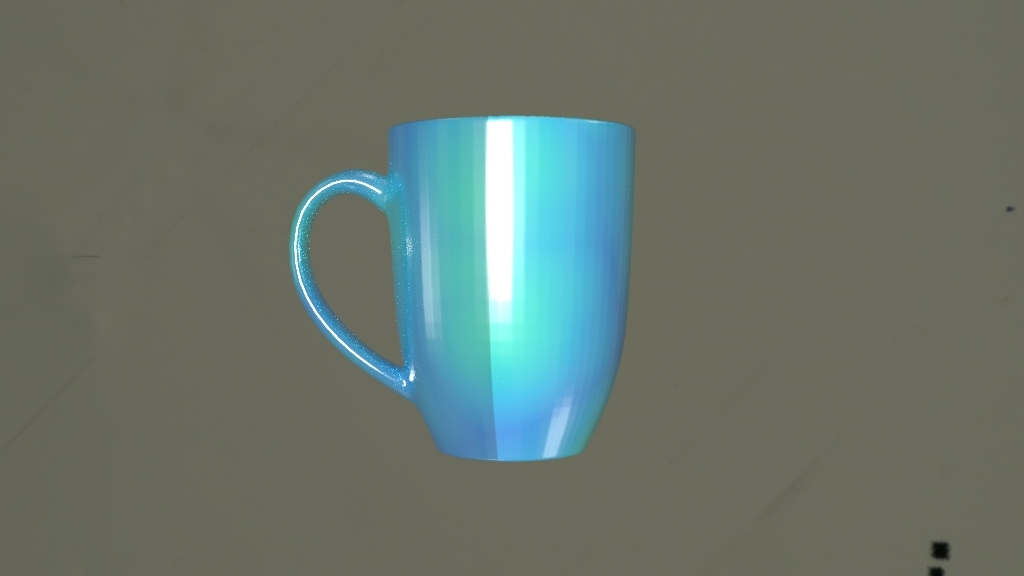
\includegraphics[width=0.1\textwidth]{interp/real_interp/cup/cup_sl}}&
\raisebox{-.5\height}{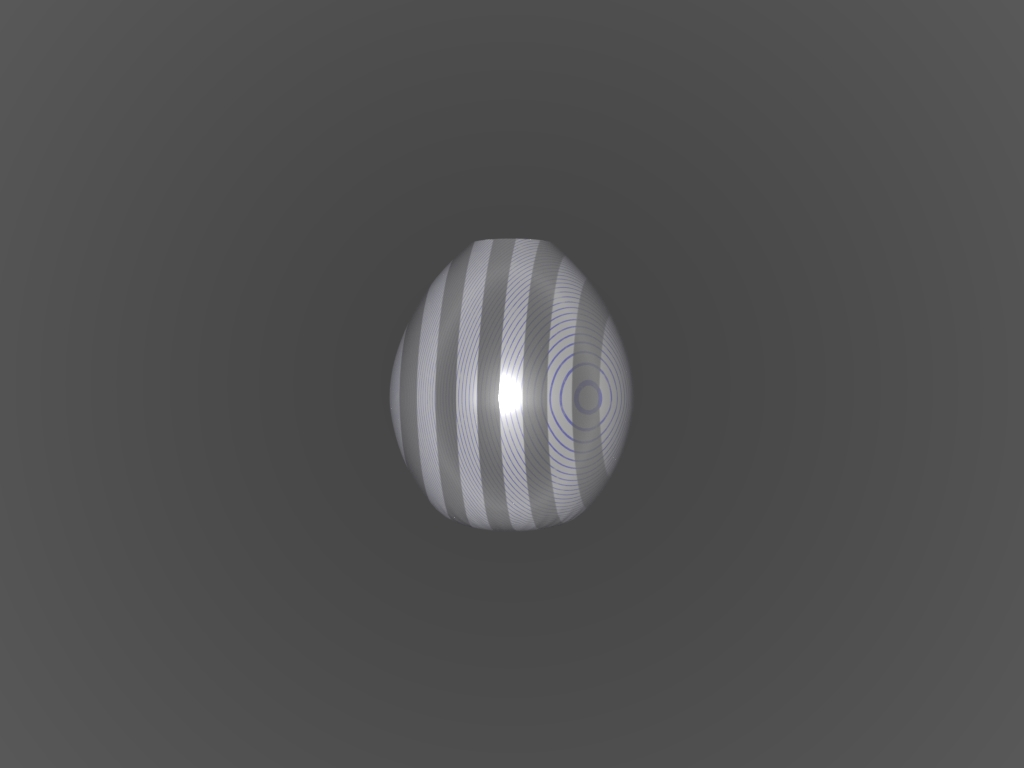
\includegraphics[width=0.1\textwidth]{interp/real_interp/pot/pot_sl}}&
\raisebox{-.5\height}{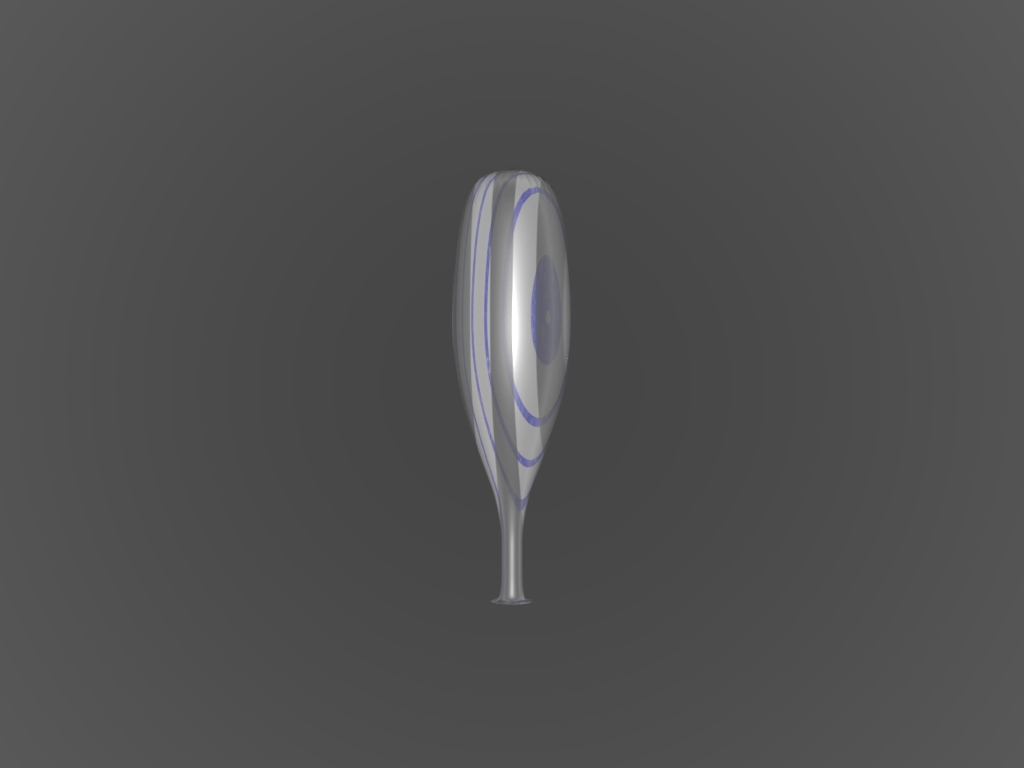
\includegraphics[width=0.1\textwidth]{interp/real_interp/vase/vase_sl}}&
GSL\\
2 &
\raisebox{-.5\height}{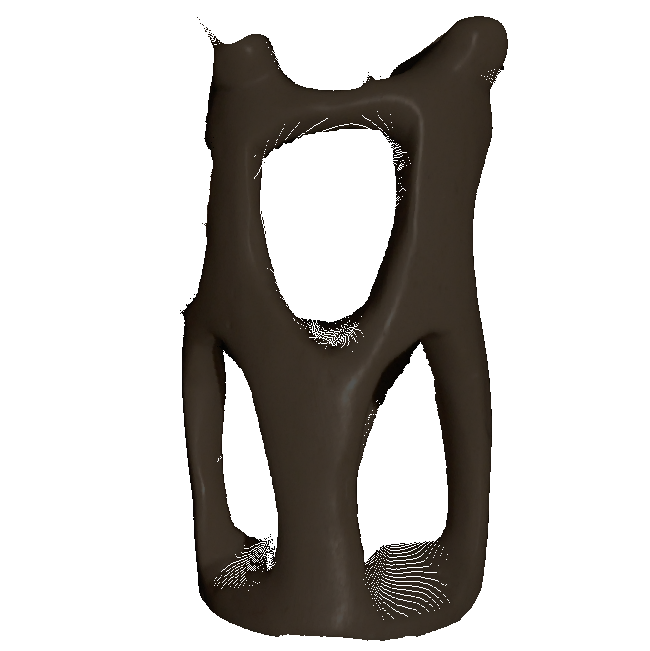
\includegraphics[width=0.1\textwidth]{interp/real_interp/statue/statue_ps}}&
\fcolorbox{green}{white}{\raisebox{-.5\height}{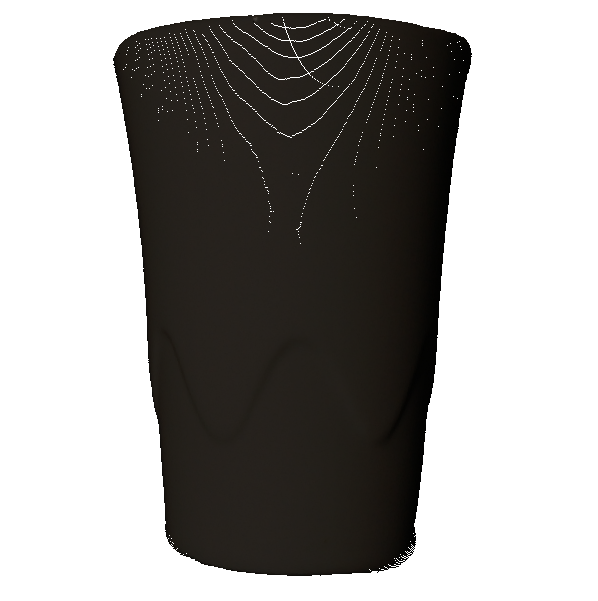
\includegraphics[width=0.1\textwidth]{interp/real_interp/cup/cup_ps}}}&
\raisebox{-.5\height}{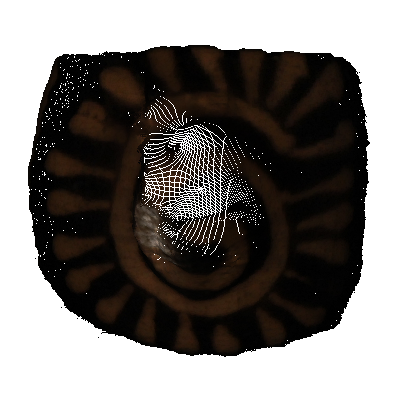
\includegraphics[width=0.1\textwidth]{interp/real_interp/pot/pot_ps}}&
\raisebox{-.5\height}{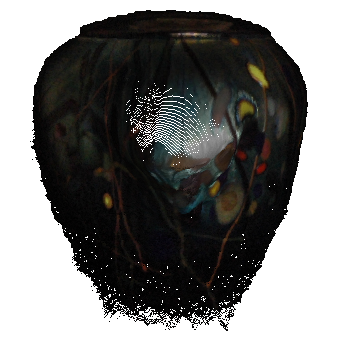
\includegraphics[width=0.1\textwidth]{interp/real_interp/vase/vase_ps}}&
EPS\\
3 &
\raisebox{-.5\height}{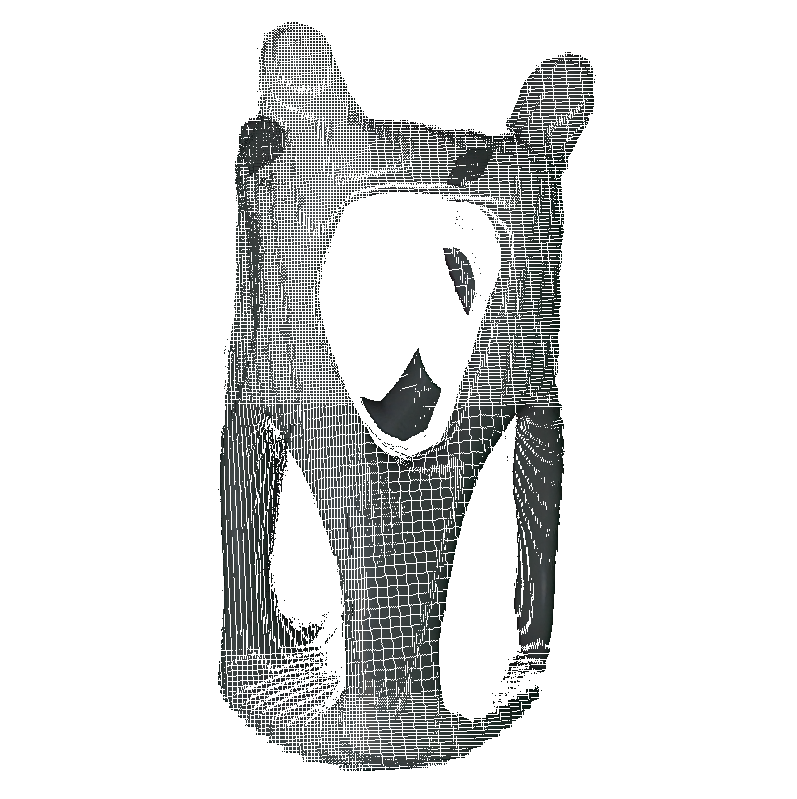
\includegraphics[width=0.1\textwidth]{interp/real_interp/statue/statue_sl}}&
\raisebox{-.5\height}{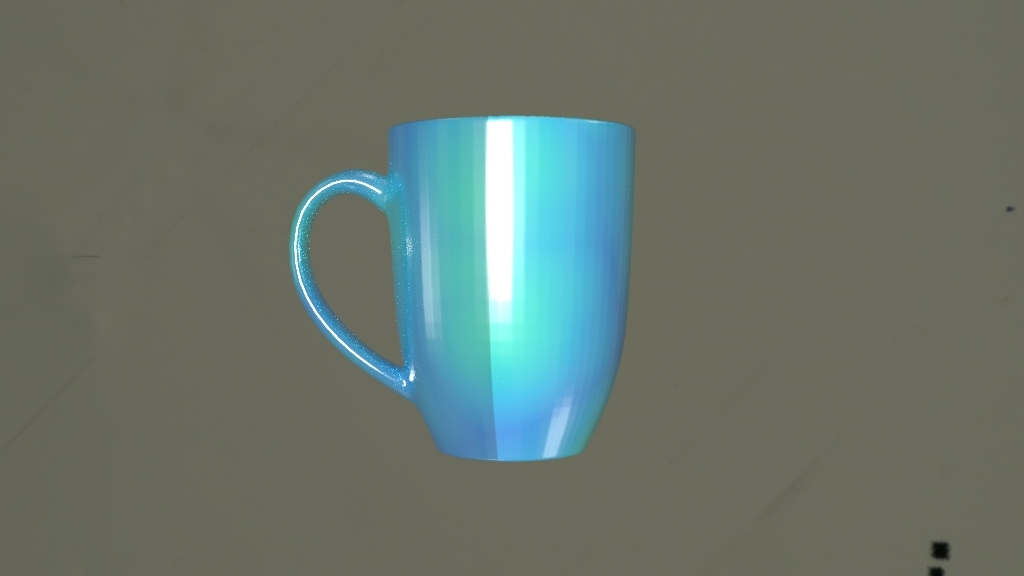
\includegraphics[width=0.1\textwidth]{interp/real_interp/cup/cup_sl}}&
\fcolorbox{green}{white}{\raisebox{-.5\height}{\includegraphics[width=0.1\textwidth]{interp/real_interp/pot/pot_sl}}}&
\raisebox{-.5\height}{\includegraphics[width=0.1\textwidth]{interp/real_interp/vase/vase_sl}}&
GSL\\
4 &
\raisebox{-.5\height}{\includegraphics[width=0.1\textwidth]{interp/real_interp/statue/statue_mvs}}&
\raisebox{-.5\height}{\includegraphics[width=0.1\textwidth]{interp/real_interp/cup/cup_mvs}}&
\raisebox{-.5\height}{\includegraphics[width=0.1\textwidth]{interp/real_interp/pot/pot_mvs}}&
\fcolorbox{green}{white}{\raisebox{-.5\height}{\includegraphics[width=0.1\textwidth]{interp/real_interp/vase/vase_mvs}}}&
PMVS\\
\bottomrule
\end{tabular}
\caption{The evaluation of interpreter using real-world objects. The first column presents the description provided to the interpreter. Description $i$ matches with condition $i$ in Table~\ref{tab:real_data_prop_list}. The last column is the algorithm selected by the interpreter. The object of which the condition matches the description is labeled in green rectangle. Since the interpreter would return a successful reconstruction given a description that matches the condition, the quality of reconstruction of the labeled objects indicate the success/failure of the interpreter.}
\label{fig:real_results}
\end{figure*}

\section{Summary}
Building upon our description and mapping, we are able to develop a proof of concept interpreter which interprets the description of the problem, selects the most appropriate algorithm based on the mapping and returns a reliable reconstruction result. The development of more complex descriptions of object geometry and material, incorporating new algorithms, and improving mapping are all ongoing processes to improve the interface presented.
